\documentclass[12pt,a4paper,oneside]{report}

%% ─── Packages ────────────────────────────────────────────────────────────────
\usepackage[utf8]{inputenc}
\usepackage[T1]{fontenc}
\usepackage[english,french]{babel}
\usepackage{lmodern}
\usepackage{microtype}

%% Layout
\usepackage[top=2.5cm,bottom=2.5cm,left=3cm,right=2.5cm]{geometry}
\usepackage{setspace}
\onehalfspacing

%% Graphics & Colors
\usepackage{graphicx}
\usepackage[table,xcdraw]{xcolor}
\usepackage{tikz}
\usetikzlibrary{shapes,arrows,arrows.meta,positioning,fit,calc,backgrounds,shadows.blur,shapes.symbols,shapes.geometric}

%% Tables
\usepackage{booktabs}
\usepackage{longtable}
\usepackage{array}
\usepackage{multirow}
\usepackage{tabularx}

%% Code listings
\usepackage{listings}
\usepackage{minted}

%% Math
\usepackage{amsmath}
\usepackage{amssymb}

%% Hyperlinks
\usepackage[colorlinks=true,
            linkcolor=blue!70!black,
            citecolor=green!50!black,
            urlcolor=blue!70!black]{hyperref}

%% Bibliography
\usepackage[backend=biber,style=ieee,sorting=none]{biblatex}
\addbibresource{bibliography/references.bib}

%% Headers & Footers
\usepackage{fancyhdr}
\pagestyle{fancy}
\fancyhf{}
\fancyhead[L]{\small\leftmark}
\fancyhead[R]{\small BVIRAL Platform}
\fancyfoot[C]{\thepage}
\renewcommand{\headrulewidth}{0.4pt}

%% Chapter style
\usepackage{titlesec}
\titleformat{\chapter}[display]
  {\normalfont\huge\bfseries\color{blue!70!black}}
  {\chaptertitlename\ \thechapter}{20pt}{\Huge}
\titlespacing*{\chapter}{0pt}{50pt}{40pt}

%% Miscellaneous
\usepackage{enumitem}
\usepackage{float}
\usepackage{caption}
\usepackage{subcaption}
\usepackage{pdfpages}
\usepackage{acronym}
\usepackage{csquotes}
\usepackage{mdframed}

%% Color definitions
\definecolor{codegreen}{rgb}{0,0.6,0}
\definecolor{codegray}{rgb}{0.5,0.5,0.5}
\definecolor{codepurple}{rgb}{0.58,0,0.82}
\definecolor{backcolour}{rgb}{0.97,0.97,0.97}
\definecolor{bviralblue}{RGB}{0,82,155}
\definecolor{bvirallightblue}{RGB}{0,153,255}

%% Listings style
\lstdefinestyle{mystyle}{
    backgroundcolor=\color{backcolour},
    commentstyle=\color{codegreen},
    keywordstyle=\color{blue}\bfseries,
    numberstyle=\tiny\color{codegray},
    stringstyle=\color{codepurple},
    basicstyle=\ttfamily\footnotesize,
    breakatwhitespace=false,
    breaklines=true,
    captionpos=b,
    keepspaces=true,
    numbers=left,
    numbersep=5pt,
    showspaces=false,
    showstringspaces=false,
    showtabs=false,
    tabsize=2,
    frame=single,
    rulecolor=\color{codegray}
}
\lstset{style=mystyle}

%% ─── Sequence Diagram Helpers ─────────────────────────────────────────────
%% Participant box styles (color-coded by service role)
\tikzset{
  sdFE/.style={draw=blue!60!black, fill=blue!10, rounded corners=3pt,
    minimum width=2.1cm, minimum height=0.58cm,
    font=\fontsize{7.5}{9}\selectfont\bfseries, align=center, text=blue!25!black},
  sdBE/.style={draw=teal!70!black, fill=teal!10, rounded corners=3pt,
    minimum width=2.1cm, minimum height=0.58cm,
    font=\fontsize{7.5}{9}\selectfont\bfseries, align=center, text=teal!25!black},
  sdExt/.style={draw=gray!60, fill=gray!8, rounded corners=3pt,
    minimum width=2.1cm, minimum height=0.58cm,
    font=\fontsize{7.5}{9}\selectfont\bfseries, align=center},
  sdData/.style={draw=violet!70, fill=violet!8, rounded corners=3pt,
    minimum width=2.1cm, minimum height=0.58cm,
    font=\fontsize{7.5}{9}\selectfont\bfseries, align=center, text=violet!30!black},
  sdWork/.style={draw=orange!70!black, fill=orange!8, rounded corners=3pt,
    minimum width=2.1cm, minimum height=0.58cm,
    font=\fontsize{7.5}{9}\selectfont\bfseries, align=center},
  %% Message arrows
  sdmsg/.style={->, >=Stealth, thick},
  sdret/.style={->, >=Stealth, semithick, dashed, gray!65},
  %% Note box (yellow sticky)
  sdnote/.style={draw=orange!60!black, fill=yellow!12, rounded corners=2pt,
    font=\fontsize{6.5}{8}\selectfont, align=center, inner sep=3pt},
  %% Fragment box label
  sdfrag/.style={draw=gray!50, fill=gray!4, rounded corners=2pt,
    font=\fontsize{7}{8}\selectfont\itshape, inner sep=2pt},
}

%% ─── Use-Case Diagram Helpers ──────────────────────────────────────────────
\tikzset{
  ucboundary/.style={draw=gray!55, fill=gray!4, rounded corners=6pt,
    dashed, thick},
  usecase/.style={draw=blue!55!black, fill=blue!8, ellipse,
    font=\fontsize{8}{9}\selectfont, align=center,
    minimum width=2.9cm, minimum height=0.68cm},
  ucassoc/.style={thick, gray!60},
  ucincl/.style={->, >=Stealth, dashed, gray!55,
    font=\fontsize{6.5}{7}\selectfont\itshape},
}

%% UML stick-figure actor: \umlactor{x}{y}{label}
\newcommand{\umlactor}[3]{%
  \begin{scope}[shift={(#1,#2)}]
    \draw[thick] (0,0.30) circle (0.17cm);
    \draw[thick] (0,0.13) -- (0,-0.20);
    \draw[thick] (-0.22,0.03) -- (0.22,0.03);
    \draw[thick] (0,-0.20) -- (-0.17,-0.52);
    \draw[thick] (0,-0.20) -- (0.17,-0.52);
    \node[font=\fontsize{8}{9}\selectfont, align=center, text width=1.8cm]
      at (0,-0.73) {#3};
  \end{scope}
}

%% ─── Document ────────────────────────────────────────────────────────────────
\begin{document}

%% Title page
\begin{titlepage}
\centering
\newgeometry{top=0.8cm,bottom=0.8cm,left=0.8cm,right=0.8cm}
\setlength{\fboxsep}{8pt}
\fbox{%
\begin{minipage}[t][0.955\textheight][t]{0.985\textwidth}
\centering

%% Top institutional block
\begin{minipage}[t]{0.30\textwidth}
  \centering
  \textbf{Tunisian Republic}\\
  \textbf{Ministry of Higher Education}\\
  \textbf{and Scientific Research}\\
  \textbf{University of Sousse}\\[0.2em]
  
\includegraphics[width=3.0cm]{figures/sousse}
\end{minipage}
\hfill
\begin{minipage}[t]{0.36\textwidth}
  \centering
  \vspace{0.3em}
  \textbf{\large IT DEPARTMENT}
\end{minipage}
\hfill
\begin{minipage}[t]{0.30\textwidth}
  \centering
  \textbf{Higher Institute of Applied}\\
  \textbf{Sciences and Technology}\\
  \textbf{of Sousse}\\[0.2em]
  
\includegraphics[width=3.0cm]{figures/logos/issat_logo}
\end{minipage}

\vspace{0.7cm}
\rule{0.9\textwidth}{1pt}\\[0.4em]
{\Large\bfseries End of Studies Project Report}\\[0.2em]
{\normalsize Presented to Obtain:}\\[0.2em]
{\large\bfseries National Diploma of Computer Engineering}\\[0.2em]
{\normalsize Option: \textit{Software Engineering -- Full Stack \& AI}}\\[0.4em]
\rule{0.9\textwidth}{1pt}

\vspace{0.8cm}
\fbox{%
\begin{minipage}{0.86\textwidth}
\centering
\vspace{0.3em}
{\LARGE\bfseries\color{bviralblue}
Distributed Video Search, Indexing \&\\[0.2em]
AI-Assisted Retrieval System
}
\vspace{0.3em}
\end{minipage}
}

\vspace{0.7cm}
\textbf{Hosting Company}\\[0.25em]

\includegraphics[width=2.9cm]{figures/logos/bviral_logo.jpeg}\\[0.2em]
\textbf{BVIRAL Media Inc.}

\vspace{0.6cm}
\textbf{Elaborated by:}\\[0.2em]
{\large Wassim Kraiem}

\vspace{0.5cm}
\textbf{Presented on: \today}

\vspace{0.5cm}
\begin{tabular}{ll}
  \textbf{Academic supervisor:}  & Mr Sofienne Ben Ahmed \\
  \textbf{Industrial supervisor:} & Mr Abdellatif Kraiem \\
\end{tabular}

\vfill
{\small Academic Year: 2025/2026 \quad Subject Code: FI-SE25-XXX}
\end{minipage}%
}
\restoregeometry
\end{titlepage}


%% Front matter
\pagenumbering{roman}
\chapter*{Dedication}
\addcontentsline{toc}{chapter}{Dedication}
\markboth{Dedication}{Dedication}

\vspace{3cm}

\begin{center}
  \itshape

  To my family, whose unwavering support and encouragement\\
  carried me through every challenge of this journey.

  \vspace{1.5cm}

  To my friends and colleagues who stood by me\\
  and believed in the value of this work.

  \vspace{1.5cm}

  To all those who face the challenge of building meaningful technology\\
  at the intersection of intelligence, creativity, and scale.

  \vspace{1.5cm}

  This work is dedicated to you.

\end{center}

\chapter*{Acknowledgements}
\addcontentsline{toc}{chapter}{Acknowledgements}
\markboth{Acknowledgements}{Acknowledgements}

At the conclusion of this work, I am pleased to express my sincere gratitude to all those who
contributed, directly or indirectly, to its completion.

I would like to extend my heartfelt thanks to my \textbf{academic supervisor} for their
invaluable guidance, constructive feedback, and continuous encouragement throughout the duration
of this project. Their expertise and dedication were instrumental in shaping the quality of
this work.

I am deeply grateful to my \textbf{industrial supervisor} at BVIRAL for providing the
professional context, technical resources, and domain knowledge necessary to tackle real-world
challenges in video content management and AI-assisted search.

To the entire \textbf{BVIRAL team}, thank you for your warm welcome, your openness in sharing
technical insights, and for creating an environment where innovation is valued and supported.

I also wish to express my appreciation to the \textbf{jury members} for agreeing to evaluate
this work and for their valuable comments and suggestions.

Finally, my deepest gratitude goes to my \textbf{family and friends} for their moral support,
patience, and encouragement during the most demanding phases of this project.

\chapter*{Abstract}
\addcontentsline{toc}{chapter}{Abstract}
\markboth{Abstract}{Abstract}

This End-of-Studies Project (PFE) was carried out in collaboration with
\textbf{BVIRAL}, a company specialized in viral video licensing. The initial
goal was practical: replace disconnected internal tools with one
production-ready platform that supports the full rights workflow.

The project delivered the \textbf{BVIRAL Platform}, built around two
complementary products: (1) a video search portal for discovering clips through
keywords, filters, and natural-language queries, and (2) an Authentic Rights
Portal for onboarding, subscription management, and licensing operations for
creators and media partners.

The platform follows a \textbf{microservices monorepo} architecture with five
independent services: AR-API (FastAPI, PostgreSQL, Celery, Stripe, Clerk),
Videos Search API (Flask, OpenSearch), Agentic Helper API (FastAPI, LangChain,
Qdrant, LangSmith), Video Search Portal (Next.js 15), and Authentic Rights
Portal (Next.js 16). Services are containerized and orchestrated with Docker
Compose.

A core contribution is the \textbf{Agentic Helper}, which combines RAG over
\textit{Qdrant}, LangSmith-managed prompts and tracing, a ReAct video-search
agent, a two-level routing classifier, and Whisper-based audio
transcription. This AI layer improves video discovery, provides contextual
support directly inside the user interfaces, and exposes admin endpoints for
managing FAQ vectors.

\bigskip
\noindent\textbf{Keywords:} Microservices; Next.js; FastAPI; Flask;
OpenSearch; LangChain; RAG; Qdrant; LangSmith; OpenAI; Stripe;
Clerk; Docker; Celery; Video search; Rights management.

\newpage
\chapter*{Summary}
\addcontentsline{toc}{chapter}{Summary}
\markboth{Summary}{Summary}

This report presents the end-to-end design and implementation of the BVIRAL
Platform as a unified system for content rights operations and AI-assisted
video discovery. The architecture separates concerns into independent
microservices, with dedicated APIs for onboarding, payments, search, and
conversational assistance.

From a software engineering perspective, the work focused on production
constraints: clear service boundaries, asynchronous background processing,
containerized deployment, and reproducible CI/CD. From an AI perspective, the
work combined retrieval-based grounding, tool-using agents, intent routing, and
speech transcription to support practical user interactions rather than demo
flows.

The resulting platform is functional in production scenarios and provides a
clear baseline for future upgrades such as multimodal retrieval, stronger LLM
evaluation, and expanded operational tooling.


%% Table of contents
\cleardoublepage
\tableofcontents

%% List of tables
\cleardoublepage
\addcontentsline{toc}{chapter}{\listtablename}
\listoftables

%% List of figures
\cleardoublepage
\addcontentsline{toc}{chapter}{\listfigurename}
\listoffigures

\chapter*{List of Abbreviations}
\addcontentsline{toc}{chapter}{List of Abbreviations}
\markboth{List of Abbreviations}{List of Abbreviations}

\begin{acronym}[OPENSEARCH]
  \acro{AI}{Artificial Intelligence}
  \acro{API}{Application Programming Interface}
  \acro{AR}{Authentic Rights}
  \acro{AWS}{Amazon Web Services}
  \acro{BFF}{Backend For Frontend}
  \acro{CI}{Continuous Integration}
  \acro{CD}{Continuous Deployment}
  \acro{CORS}{Cross-Origin Resource Sharing}
  \acro{CRUD}{Create, Read, Update, Delete}
  \acro{CSS}{Cascading Style Sheets}
  \acro{DB}{Database}
  \acro{DI}{Dependency Injection}
  \acro{DML}{Data Manipulation Language}
  \acro{DTO}{Data Transfer Object}
  \acro{ECR}{Elastic Container Registry}
  \acro{ECS}{Elastic Container Service}
  \acro{HTTP}{Hypertext Transfer Protocol}
  \acro{IDE}{Integrated Development Environment}
  \acro{IaC}{Infrastructure as Code}
  \acro{JWT}{JSON Web Token}
  \acro{JSON}{JavaScript Object Notation}
  \acro{LCEL}{LangChain Expression Language}
  \acro{LLM}{Large Language Model}
  \acro{MUI}{Material UI}
  \acro{ORM}{Object-Relational Mapping}
  \acro{PFE}{Projet de Fin d'Études (End-of-Studies Project)}
  \acro{RAG}{Retrieval-Augmented Generation}
  \acro{ReAct}{Reasoning and Acting (agent paradigm)}
  \acro{REST}{Representational State Transfer}
  \acro{SaaS}{Software as a Service}
  \acro{SDK}{Software Development Kit}
  \acro{SMS}{Social Media Scraper (internal service)}
  \acro{SQL}{Structured Query Language}
  \acro{SSM}{AWS Systems Manager Parameter Store}
  \acro{SSR}{Server-Side Rendering}
  \acro{TLS}{Transport Layer Security}
  \acro{UI}{User Interface}
  \acro{UML}{Unified Modeling Language}
  \acro{URL}{Uniform Resource Locator}
  \acro{UUID}{Universally Unique Identifier}
  \acro{WSGI}{Web Server Gateway Interface}
  \acro{ASGI}{Asynchronous Server Gateway Interface}
  \acro{OPENSEARCH}{OpenSearch (distributed search engine)}
\end{acronym}

\cleardoublepage

%% Main matter
\pagenumbering{arabic}
\chapter*{General Introduction}
\addcontentsline{toc}{chapter}{General Introduction}
\markboth{General Introduction}{General Introduction}

\section*{Context and Motivation}

Short-form video is now the dominant content format on social media, and that creates real friction for media companies. News outlets, broadcasters, and digital publishers need a constant supply of licensed footage, often viral clips captured by ordinary people on Instagram, TikTok, and YouTube. Yet finding a clip, verifying ownership, negotiating rights, and delivering files still relies heavily on email threads, spreadsheets, and manual follow-ups.

\textbf{BVIRAL} is a media technology company that licenses viral video content. The company sits between the people who shoot the footage and the organizations that want to publish it. As the catalogue grew and the client base expanded, the collection of internal scripts and disconnected SaaS tools that ran the business stopped scaling.

This project replaces that patchwork with a \textbf{unified, API-first platform} that covers the full lifecycle of a video rights transaction, from creator channel submission, through subscription payment and digital agreement, to catalogue search with AI assistance when keyword search is not enough.

\section*{Problem Statement}

Before this project, BVIRAL had four concrete operational gaps:

\begin{itemize}
  \item \textbf{Manual onboarding}: Creators and media partners had no self-service flow. Every new account required staff intervention for channel review, payment coordination, and access provisioning.
  \item \textbf{Weak search}: The video catalogue was searchable only by keyword. Queries like "a crowd celebrating a football goal" returned nothing useful.
  \item \textbf{No conversational interface}: Users couldn't describe what they were looking for in plain language or ask support questions without waiting for a human response.
  \item \textbf{Operational silos}: Authentication, payments, video indexing, and customer support ran as separate tools with no shared data model or unified API.
\end{itemize}

\section*{Proposed Solution}

This End-of-Studies Project delivers the \textbf{BVIRAL Platform}, a microservices monorepo with five production-grade services:

\begin{enumerate}
  \item \textbf{AR-API}: FastAPI backend handling user lifecycle, onboarding, Stripe payments, Celery background jobs, and media library access provisioning.
  \item \textbf{Videos Search API}: Flask/OpenSearch service for full-text, semantic, and faceted video search.
  \item \textbf{Agentic Helper API}: LangChain service providing a RAG chatbot, a video-search ReAct agent, a two-level routing classifier, and speech transcription.
  \item \textbf{Video Search Portal}: Next.js 15 public portal for video discovery.
  \item \textbf{Authentic Rights Portal}: Next.js 16 SaaS dashboard for subscription and rights management.
\end{enumerate}

\section*{Report Structure}

This report is organized into eight chapters followed by a general conclusion:

\begin{itemize}
  \item \textbf{Chapter 1} covers the host organization, the business context, a comparison with existing solutions, and the development methodology.
  \item \textbf{Chapter 2} specifies functional and non-functional requirements and presents the global use-case models (Sprint 0).
  \item \textbf{Chapter 3} details Sprint 1: user authentication, creator onboarding flow, Stripe subscription payments, and Canto DAM integration.
  \item \textbf{Chapter 4} details Sprint 2: video document ingestion, OpenSearch index mapping, keyword search, and faceted filtering.
  \item \textbf{Chapter 5} details Sprint 3: embedding pipeline, kNN vector search, parallel retrieval, RRF fusion, and position-aware ranking.
  \item \textbf{Chapter 6} details Sprint 4: the Agentic Helper's Qdrant-backed RAG layer, two-level classifier pipeline, prompt engineering, and sliding-window memory.
  \item \textbf{Chapter 7} details Sprint 5: the structured search orchestrator, ReAct agent fallback, Whisper voice transcription, FAQ administration, and portal integration.
  \item \textbf{Chapter 8} details Sprint 6: the personalized recommendation engine, per-user interest profiles with weight decay, blended candidate pipeline, and anti-repetition ranking.
\end{itemize}

\chapter{General Project Presentation}

\section*{Introduction}
\addcontentsline{toc}{section}{Introduction}

This chapter introduces the host organization, frames the project context, compares the BVIRAL
Platform with existing market solutions, and presents the Agile methodology, the sprint planning,
and the overall timeline followed during the project.

%% ─── 1.1 ─────────────────────────────────────────────────────────────────────
\section{Presentation of the Host Organization}

\subsection{BVIRAL Media Inc.}

\textbf{BVIRAL} is a digital media company that licenses viral video content. It acts as an
intermediary between \textit{content creators}, individuals who capture footage on Instagram,
TikTok, YouTube, and Facebook, and \textit{media buyers}, such as news outlets, broadcasters,
publishers, and advertising agencies that need licensed footage for production.

BVIRAL's business model includes:

\begin{itemize}
  \item Discovering and curating high-engagement video clips from social media.
  \item Acquiring exclusive or non-exclusive licensing rights from creators.
  \item Indexing content for fast retrieval.
  \item Sub-licensing to media partners through a SaaS subscription.
\end{itemize}

The platform developed in this project serves both sides of this marketplace through two front-end
portals backed by a shared API layer.

\subsection{Technical Environment Before This Project}

Before the unified BVIRAL Platform, the company relied on a mix of internal scripts and external
SaaS tools, each managing a separate part of the business (creator management, payments, video
archives). There was no shared data model, no self-service onboarding, and onboarding a new client
required manual work across multiple systems.

%% ─── 1.2 ─────────────────────────────────────────────────────────────────────
\section{Project Presentation}

\subsection{Objectives}

This project was commissioned to design and build a unified, production-ready platform that:

\begin{enumerate}
  \item Automates the creator/partner \textbf{onboarding journey} end-to-end, from channel
    submission through Stripe payment to media library access provisioning.
  \item Provides a \textbf{video search engine} backed by OpenSearch with semantic and faceted
    search capabilities.
  \item Integrates an \textbf{AI assistant} that understands natural language search requests,
    answers support questions via RAG, and transcribes audio queries.
  \item Delivers a \textbf{personalized recommendation engine} that learns from each user's
    search queries and click events to build a continuously updated interest profile, driving
    a blended feed of personalized and trending videos.
  \item Exposes all functionality through clean, versioned \textbf{REST APIs} consumed by both
    portals and third-party integrations.
\end{enumerate}

\subsection{Problem Dimensions}

\begin{table}[H]
\centering
\caption{Problem dimensions and their impact}
\begin{tabularx}{\textwidth}{>{\bfseries}lX}
\toprule
Dimension & Description \\
\midrule
Operational & Manual creator onboarding took days and was error-prone, causing revenue leakage
              and poor first impressions. \\[0.5em]
Search quality & Keyword-only search failed for natural language queries (e.g., ``a football
                 crowd celebrating''). \\[0.5em]
AI capability & No conversational interface existed; users with complex requests had to wait
                for a human response. \\[0.5em]
Scalability & Without service separation, it was impossible to scale the search layer
              independently from billing. \\
\bottomrule
\end{tabularx}
\end{table}

\subsection{Proposed Solution Overview}

The solution is a microservices platform deployed with Docker Compose locally and on AWS ECS in
production, comprising the five services in Table~\ref{tab:services}.

\begin{table}[H]
\centering
\caption{BVIRAL Platform services overview}
\label{tab:services}
\small
\renewcommand{\arraystretch}{1.15}
\begin{tabularx}{\textwidth}{>{\raggedright\arraybackslash}p{0.24\textwidth} >{\raggedright\arraybackslash}p{0.31\textwidth} >{\raggedright\arraybackslash}X}
\toprule
\textbf{Service} & \textbf{Technology} & \textbf{Responsibility} \\
\midrule
AR-API & FastAPI, PostgreSQL,\\ Celery, Redis & User management, onboarding, payments, and channels. \\
Videos Search API & Flask, OpenSearch & Video indexing, full-text search, and semantic search. \\
Agentic Helper & FastAPI, LangChain,\\ Qdrant, LangSmith & RAG chatbot, video search agent, transcription, and prompt tracing. \\
Video Search Portal & Next.js 15, Clerk,\\ Radix UI & Public video discovery interface. \\
Authentic Rights Portal & Next.js 16, MUI,\\ Clerk, Stripe & SaaS dashboard, onboarding, and subscription flows. \\
\bottomrule
\end{tabularx}
\normalsize
\end{table}

%% ─── 1.3 ─────────────────────────────────────────────────────────────────────
\section{Study of Existing Solutions}

\subsection{Competing Platforms}

\begin{table}[H]
\centering
\caption{Comparative analysis of existing solutions}
\begin{tabularx}{\textwidth}{lXXX}
\toprule
\textbf{Platform} & \textbf{Video Search} & \textbf{Rights Mgmt.} & \textbf{AI Assistant} \\
\midrule
Getty Images       & Advanced keyword + AI & Full licensing suite & Partial \\
Storyful           & Social media monitoring & Manual licensing & No \\
Jukin Media        & Curated catalogue & Subscription-based & No \\
Shutterstock Video & Semantic + keyword & Standard subscription & Partial \\
\textbf{BVIRAL Platform} & \textbf{Semantic + ReAct agent} & \textbf{Automated SaaS} & \textbf{Full RAG + Agent} \\
\bottomrule
\end{tabularx}
\end{table}

The BVIRAL Platform stands out because the agentic AI layer and rights management pipeline live in
the same platform and share one user identity model. None of the compared platforms offer this
combination.

%% ─── 1.4 ─────────────────────────────────────────────────────────────────────
\section{Working Methodology}

\subsection{Adopted Methodology}

Given the exploratory nature of the project and the frequent feedback cycles with the industrial
supervisor, an \textbf{Agile} approach organized into two-week sprints was selected. Each sprint
followed a structured ceremony loop: planning, daily development, review, and retrospective.
The product backlog was continuously prioritized in collaboration with the supervisor to reflect
evolving business priorities.

%% ── Classic vs Agile ──────────────────────────────────────────────────────────
\subsection{Classic vs.\ Agile Methodology}

\begin{table}[H]
\centering
\caption{Comparative study: Classic (Waterfall) vs.\ Agile methodology}
\label{tab:method_compare}
\renewcommand{\arraystretch}{1.25}
\begin{tabularx}{\textwidth}{>{\bfseries}lXX}
\toprule
Criterion & Classic (Waterfall) & Agile \\
\midrule
Delivery model    & Single final release at project end              & Incremental releases every sprint \\
Flexibility       & Changes are costly once a phase is closed        & Changes welcomed at any sprint boundary \\
Customer feedback & Collected only at the end                        & Integrated after every sprint review \\
Risk management   & Late discovery of integration problems           & Risks surfaced and resolved each sprint \\
Documentation     & Heavy upfront specification                      & Lightweight, just-enough documentation \\
Team collaboration & Sequential hand-offs between roles              & Cross-functional team, daily collaboration \\
Suitability       & Well-defined, stable-requirement projects        & Evolving requirements, innovation projects \\
\bottomrule
\end{tabularx}
\end{table}

Classic methodologies follow a rigid, phase-by-phase pipeline (requirements $\rightarrow$ design
$\rightarrow$ implementation $\rightarrow$ testing $\rightarrow$ deployment) where each phase must
be fully completed before the next begins. While predictable for well-scoped projects, this model
struggles when requirements evolve — a common reality in platform development. Agile addresses
this by splitting work into short cycles, producing a working increment at the end of each one,
and adapting the plan based on real feedback.

%% ── Agile → Scrum ────────────────────────────────────────────────────────────
\subsection{From Agile to Scrum}

\textbf{Scrum} is the most widely adopted Agile framework. It operationalizes Agile values into
a concrete, repeatable process built around three pillars — \textit{transparency},
\textit{inspection}, and \textit{adaptation} — and three core roles:

\begin{itemize}
  \item \textbf{Product Owner:} owns the product backlog, prioritizes user stories, and
    validates that each increment delivers business value. In this project, this role was held
    by the industrial supervisor.

  \item \textbf{Scrum Master:} facilitates ceremonies, removes impediments, and ensures the
    team adheres to Scrum principles. This role was fulfilled by the project intern.

  \item \textbf{Development Team:} a self-organizing group that designs, implements, tests,
    and integrates features to produce a \textit{potentially shippable increment} each sprint.
\end{itemize}

Figure~\ref{fig:scrum} illustrates the Scrum cycle adopted throughout this project.

\begin{figure}[H]
\centering
\resizebox{0.98\textwidth}{!}{%
\begin{tikzpicture}[
  node distance=1.05cm and 0.95cm,
  stage/.style={draw=blue!55!black, fill=blue!8, rounded corners=5pt,
                minimum width=3.0cm, minimum height=1.05cm,
                inner xsep=8pt, inner ysep=6pt,
                font=\small, align=center},
  arr/.style={->, >=Stealth, thick, blue!60!black, rounded corners=4pt}
]
\node[stage] (pb) {Product\\Backlog};
\node[stage, right=of pb] (sp) {Sprint\\Planning};
\node[stage, right=of sp] (sb) {Sprint\\Backlog};
\node[stage, right=of sb] (dev) {Development\\(2-week sprint)};
\node[stage, below=of dev] (rev) {Sprint Review\\+ Retrospective};
\node[stage, left=of rev] (inc) {Potentially Shippable\\Increment};

\draw[arr] (pb) -- (sp);
\draw[arr] (sp) -- (sb);
\draw[arr] (sb) -- (dev);
\draw[arr] (dev) -- (rev);
\draw[arr] (rev) -- (inc);
\draw[arr] (inc.south) -- ++(0,-0.45) -| (pb.south);
\end{tikzpicture}%
}
\caption{Adopted Scrum-inspired development process}
\label{fig:scrum}
\end{figure}

\subsection{Modeling Language: UML}

System modeling used \textbf{UML 2.x}:
\begin{itemize}
  \item Use-case diagrams for functional scope.
  \item Sequence diagrams for key interaction flows.
  \item ER diagrams for the data model.
  \item Component and deployment diagrams for the architecture.
\end{itemize}

%% ─── 1.5 ─────────────────────────────────────────────────────────────────────
\section{Sprint Planning}

The work was split into one requirements sprint (Sprint 0) followed by four implementation sprints.
Table~\ref{tab:sprint_plan} summarizes each sprint name and the delivered outcomes.

\begin{table}[H]
\centering
\caption{Sprint planning for the BVIRAL Platform}
\label{tab:sprint_plan}
\begin{tabularx}{\textwidth}{l>{\raggedright\arraybackslash}p{0.28\textwidth}X}
\toprule
\textbf{Sprint} & \textbf{Sprint name} & \textbf{What's done} \\
\midrule
Sprint 0 & Requirements and Project Setup & Defined actors and use cases, wrote the initial product backlog, validated architecture choices, and prepared the development environment. \\
Sprint 1 & Onboarding, Auth, and Billing Core & Implemented authentication and onboarding workflows, integrated Stripe subscription payment, added AR-API background processing with Celery tasks, and delivered the Authentic Rights Portal front-end with billing admin workspace. \\
Sprint 2 & Video Indexing and Full-Stack Search & Delivered OpenSearch ingestion, BM25 keyword search, and facet filters (Part A), then added semantic embeddings, kNN vector retrieval, parallel hybrid search, and position-aware rank fusion (Part B); also delivered the Video Search Portal front-end and playlist views. \\
Sprint 3 & Agentic Helper: RAG, Classification, Search Orchestration and Voice Transcription & Built the RAG pipeline with Qdrant, two-level routing/classification, and conversational memory (Phase A), then upgraded to the v2 deterministic orchestrator, Agentic RAG with CRAG-pattern re-retrieval, FAQ vector administration, and the Whisper voice transcription endpoint (Phase B); also delivered voice input, the shared ChatbotWidget, and AI-backed admin tools in both portals. \\
Sprint 4 & Personalized Recommendation Engine & Implemented user-interest profiling from events, candidate generation + blending, trending integration, and anti-repetition ranking in recommendations. \\
\bottomrule
\end{tabularx}
\end{table}

%% ─── 1.6 ─────────────────────────────────────────────────────────────────────
\section{Project Timeline}

The Gantt chart in Figure~\ref{fig:gantt} shows the planned distribution of the five sprints over
the project duration.

\begin{figure}[H]
\centering
\resizebox{0.98\textwidth}{!}{%
\begin{tikzpicture}[x=0.9cm, y=0.55cm,
  bar/.style={draw=blue!55!black, fill=blue!25, rounded corners=2pt},
  bar0/.style={draw=orange!60!black, fill=orange!25, rounded corners=2pt},
  lbl/.style={font=\footnotesize, anchor=east},
  wk/.style={font=\footnotesize\itshape, anchor=south},
  axis/.style={gray!60}
]
%% Horizontal axis: 16 weeks
\foreach \x in {0,...,16} {
  \draw[axis, dashed] (\x,-0.3) -- (\x,-6.7);
}
\foreach \x/\w in {0/W1, 2/W3, 4/W5, 6/W7, 8/W9, 10/W11, 12/W13, 14/W15, 16/W17} {
  \node[wk] at (\x,0.1) {\w};
}

%% Sprint bars (start, end, y, style, label)
\draw[bar0] (0,-0.8)   rectangle (2,-1.4);   \node[lbl] at (-0.2,-1.1) {Sprint 0};
\draw[bar]  (2,-1.8)   rectangle (5,-2.4);   \node[lbl] at (-0.2,-2.1) {Sprint 1};
\draw[bar]  (5,-2.8)   rectangle (8,-3.4);   \node[lbl] at (-0.2,-3.1) {Sprint 2};
\draw[bar]  (8,-3.8)   rectangle (11,-4.4);  \node[lbl] at (-0.2,-4.1) {Sprint 3};
\draw[bar]  (11,-4.8)  rectangle (14,-5.4);  \node[lbl] at (-0.2,-5.1) {Sprint 4};
\end{tikzpicture}%
}
\caption{Gantt chart of the project sprints}
\label{fig:gantt}
\end{figure}

For clarity, the concrete work completed in each sprint is summarized below:
\begin{itemize}
  \item \textbf{Sprint 0}: Defined actors and use cases, prepared the initial product backlog,
    validated the target architecture, and set up the development environment.
  \item \textbf{Sprint 1}: Implemented authentication and onboarding flows, integrated Stripe
    subscriptions, added AR-API background processing with Celery tasks, and delivered the
    Authentic Rights Portal front-end with a billing and moderation admin workspace.
  \item \textbf{Sprint 2}: Delivered OpenSearch ingestion, BM25 keyword search, facet-based
    filtering (Part A), then semantic embeddings, kNN retrieval, parallel hybrid search, and
    position-aware rank fusion (Part B); also delivered the Video Search Portal front-end and
    playlist management views.
  \item \textbf{Sprint 3}: Built the Agentic Helper RAG foundation with Qdrant retrieval,
    routing/classification, and conversation memory (Phase A), then upgraded to the v2
    deterministic orchestrator, Agentic RAG pipeline, and the Whisper voice transcription
    endpoint (Phase B); also delivered portal-side voice input, the shared ChatbotWidget, and
    AI-backed admin tools (conversation supervision, chatbot tester, FAQ manager).
  \item \textbf{Sprint 4}: Implemented recommendation event tracking, user-interest profiling,
    candidate blending, trending integration, and anti-repetition ranking.
\end{itemize}

\section*{Conclusion}
\addcontentsline{toc}{section}{Conclusion}

This chapter presented BVIRAL as host organization, the specific problems addressed by the
project, the comparative position of the platform against market solutions, and the Scrum-based
sprint plan that drove development. The next chapter enters Sprint 0 and specifies the detailed
requirements, actors, product backlog, work tools, and general architecture.

\chapter{Sprint 0: Requirements Specification}

\section*{Introduction}
\addcontentsline{toc}{section}{Introduction}

Sprint 0 is a discovery and preparation sprint. This chapter identifies the system actors, lists
the functional and non-functional requirements, organizes them into a product backlog, describes
the work tools adopted by the team, and defines the general architecture together with static and
dynamic design views that guide the implementation sprints.

%% Clickable back-reference to a webography item: \webref{web:fastapi}
\newcommand{\webref}[1]{\hyperref[#1]{[ref.~\ref*{#1}]}}

\newcommand{\toollogo}[3][2.0cm]{%
  \begin{figure}[H]
  \centering
  \includegraphics[height=#1,keepaspectratio]{#2}\\[0.3em]
  {\small\textbf{#3}}
  \end{figure}
}

\newcommand{\toollogotriple}[6]{%
  \begin{figure}[H]
  \centering
  \begin{minipage}[t]{0.28\textwidth}
    \centering
    \includegraphics[height=1.45cm,keepaspectratio]{#1}\\[0.25em]
    {\small\textbf{#2}}
  \end{minipage}
  \hfill
  \begin{minipage}[t]{0.28\textwidth}
    \centering
    \includegraphics[height=1.45cm,keepaspectratio]{#3}\\[0.25em]
    {\small\textbf{#4}}
  \end{minipage}
  \hfill
  \begin{minipage}[t]{0.28\textwidth}
    \centering
    \includegraphics[height=1.45cm,keepaspectratio]{#5}\\[0.25em]
    {\small\textbf{#6}}
  \end{minipage}
  \end{figure}
}

\newcommand{\toollogodouble}[4]{%
  \begin{figure}[H]
  \centering
  \begin{minipage}[t]{0.38\textwidth}
    \centering
    \includegraphics[height=1.55cm,keepaspectratio]{#1}\\[0.25em]
    {\small\textbf{#2}}
  \end{minipage}
  \hfill
  \begin{minipage}[t]{0.38\textwidth}
    \centering
    \includegraphics[height=1.55cm,keepaspectratio]{#3}\\[0.25em]
    {\small\textbf{#4}}
  \end{minipage}
  \end{figure}
}

%% ─── 2.1 ─────────────────────────────────────────────────────────────────────
\section{System Actors}

The BVIRAL Platform has four actor types:

\begin{table}[H]
\centering
\caption{System actors and their roles}
\begin{tabularx}{\textwidth}{lX}
\toprule
\textbf{Actor} & \textbf{Description} \\
\midrule
\textbf{Anonymous Visitor} & Any unauthenticated user who can browse the video portal, search
  for clips, and interact with the chatbot assistant. \\[0.4em]
\textbf{Auth. Creator / Partner} & A registered user who has completed onboarding and holds an
  active subscription. Can access the dashboard, manage playlists, submit videos, and use
  the billing portal. \\[0.4em]
\textbf{Administrator} & Internal BVIRAL staff with elevated access to review custom quote
  requests, manage pricing, and view admin reports. \\[0.4em]
\textbf{External System} & Stripe (payment webhooks), Clerk (authentication tokens), DAM
  provider APIs (media access provisioning), and the SMS Scraper API (social media follower data). \\
\bottomrule
\end{tabularx}
\end{table}

%% ─── 2.2 ─────────────────────────────────────────────────────────────────────
\section{Functional Requirements}

\subsection{Video Search Portal}

\begin{enumerate}[label=\textbf{FR-VP-\arabic*}]
  \item Browse the video catalogue with pagination and category filtering.
  \item Search videos by keyword or semantic query.
  \item View detailed video information: title, duration, category, resolution, tags.
  \item Play video previews directly in the browser.
  \item Access an embedded AI chatbot for natural language queries.
  \item Transcribe spoken audio queries via the microphone.
  \item View the latest and trending clips on the homepage.
  \item View a personalized \textbf{Recommended for You} section on the homepage, driven by
    the user's past searches and click events.
  \item Save videos to favorites and remove them; view the full favorites list.
\end{enumerate}

\subsection{Authentic Rights Portal (Onboarding and Dashboard)}

\begin{enumerate}[label=\textbf{FR-AR-\arabic*}]
  \item Submit social media channel URLs (Instagram, TikTok, YouTube, Facebook, Twitter/X,
    Snapchat) to begin onboarding.
  \item Receive automatic follower count analysis; channels over 2M followers trigger a
    custom pricing flow.
  \item Select a monthly or yearly subscription plan and complete Stripe embedded checkout.
  \item Sign the digital service agreement before checkout; receive a signed PDF by email.
  \item Complete account setup (name, account type, password) after successful payment.
  \item Access a personal dashboard with subscription status, renewal alerts, and billing portal.
  \item Manage playlists: create, rename, add or remove videos.
  \item Browse and search the licensed video \textbf{library}: filter by keyword and category,
    view video details, and download licensed clips.
  \item Manage \textbf{favorites}: add or remove videos and view the full favorites list.
  \item Submit new video clips for licensing review.
  \item Interact with the embedded AI support chatbot.
  \item \textit{Administrator}: review pending custom quote requests and set pricing.
  \item \textit{Administrator}: access whitelist reports and subscription announcements.
  \item \textit{Administrator}: browse and inspect all user chat conversations.
  \item \textit{Administrator}: test the AI chatbot directly from an admin console.
  \item \textit{Administrator}: manage the FAQ knowledge base — add, edit, search, and delete
    FAQ entries ingested into the RAG knowledge base.
  \item \textit{Administrator}: review submitted video clips and update their status.
\end{enumerate}

\subsection{Agentic Helper}

\begin{enumerate}[label=\textbf{FR-AH-\arabic*}]
  \item Accept chat messages and route them by intent (RAG, direct LLM, or video-search mode).
  \item Retrieve relevant knowledge chunks via Qdrant cosine similarity for support queries.
  \item Extract structured search filters (category, tags, duration, resolution, orientation)
    from free-text queries and execute a \textbf{deterministic advanced search} against the
    Videos Search API as the primary video-search path.
  \item Fall back to the \textbf{ReAct video-search agent} when the deterministic
    search service is unavailable.
  \item Return video results with a search URL for direct portal navigation.
  \item Ingest knowledge documents (JSON or Excel) into the RAG knowledge base.
  \item Add, update, search, and delete individual FAQ entries in the RAG knowledge base via
    dedicated admin endpoints.
  \item Transcribe audio input using OpenAI Whisper.
  \item Maintain per-user conversation history with a configurable memory window.
\end{enumerate}

%% ─── 2.3 ─────────────────────────────────────────────────────────────────────
\section{Non-Functional Requirements}

\begin{table}[H]
\centering
\caption{Non-functional requirements}
\begin{tabularx}{\textwidth}{lX}
\toprule
\textbf{Category} & \textbf{Requirement} \\
\midrule
\textbf{Performance} & Video search returns results within 500\,ms at the 95th percentile.
  Chat responses begin streaming within 2 seconds. \\[0.3em]
\textbf{Scalability} & Each microservice scales independently via container replicas.
  OpenSearch supports horizontal shard scaling. Celery workers add capacity on demand. \\[0.3em]
\textbf{Availability} & Target uptime of 99.5\% in production. Services expose \texttt{/health}
  and \texttt{/health} endpoint for load-balancer probes. \\[0.3em]
\textbf{Security} & All endpoints require authentication (Clerk JWT Bearer or API key). Stripe
  webhook payloads are verified with HMAC. Secrets are stored in per-service \texttt{.env}
  files, excluded from version control via \texttt{.gitignore}; nothing sensitive is committed
  to the repository. \\[0.3em]
\textbf{Maintainability} & Domain-driven module structure (\texttt{router → services → models}).
  Alembic manages all schema changes. Prompts are versioned text files. \\[0.3em]
\textbf{Observability} & Sentry error tracking in production for all Python services.
  All Celery tasks include retry/backoff metadata. \\[0.3em]
\textbf{Portability} & The full stack runs with a single \texttt{docker compose up} command, with no manual environment setup required. \\
\bottomrule
\end{tabularx}
\end{table}

%% ─── 2.4 ─────────────────────────────────────────────────────────────────────
\section{Use-Case Diagrams}

\subsection{Global Use-Case Diagram}

Figure~\ref{fig:uc_global} shows all system use cases grouped by portal, with the human and
system actors that interact with each.

\begin{figure}[H]
\centering

\includegraphics[width=\textwidth]{\detokenize{diagrams/global use.drawio.png}}
\caption{Global use-case diagram of the BVIRAL Platform}
\label{fig:uc_global}
\end{figure}

%% ─── 2.5 ─────────────────────────────────────────────────────────────────────
\section{Product Backlog}

The product backlog groups the functional requirements into user stories organized per epic and
prioritized with the industrial supervisor. Priority levels follow the MoSCoW convention
(\textbf{M}ust have, \textbf{S}hould have, \textbf{C}ould have).

\small
\begin{longtable}{@{}llp{0.52\textwidth}c@{}}
\caption{Product backlog (user stories per epic)}
\label{tab:product_backlog} \\
\toprule
\textbf{ID} & \textbf{Epic} & \textbf{User story} & \textbf{Prio.} \\
\midrule
\endfirsthead
\multicolumn{4}{c}{\tablename~\thetable{} — \textit{continued}} \\
\toprule
\textbf{ID} & \textbf{Epic} & \textbf{User story} & \textbf{Prio.} \\
\midrule
\endhead
\midrule
\multicolumn{4}{r}{\textit{Continued on next page}} \\
\endfoot
\bottomrule
\endlastfoot
\multicolumn{4}{l}{\textit{Sprint 1 — Authentication, Onboarding and Payments}} \\
\midrule
US-01 & Authentication  & As a visitor, I want to sign in through Clerk so that I can access
  the rights portal. & M \\
US-02 & Onboarding      & As a creator, I want to submit my social channels so the platform can
  analyze my reach. & M \\
US-03 & Onboarding      & As a creator with $>$2M followers, I want a custom-quote flow so that
  pricing can be negotiated. & S \\
US-04 & Payments        & As a user, I want to complete Stripe embedded checkout and sign the
  service agreement before payment. & M \\
US-05 & Notifications   & As a user, I want to receive a confirmation email with a signed PDF
  once payment is captured. & M \\
US-06 & Dashboard       & As a subscriber, I want a dashboard showing subscription status,
  renewal date, and a billing-portal link. & M \\
\midrule
\multicolumn{4}{l}{\textit{Sprint 2 — Video Indexing and Keyword Search}} \\
\midrule
US-07 & Video search    & As a visitor, I want keyword-based video search with filters
  (category, duration, resolution). & M \\
US-08 & Video search    & As a visitor, I want to browse the catalogue by category with
  pagination. & M \\
\midrule
\multicolumn{4}{l}{\textit{Sprint 3 — Semantic and Parallel Search with Ranking}} \\
\midrule
US-09 & Video search    & As a visitor, I want semantic search so natural-language queries work
  even without matching keywords. & M \\
US-10 & Video search    & As a visitor, I want a hybrid ranking that combines lexical and
  semantic signals for better relevance. & S \\
\midrule
\multicolumn{4}{l}{\textit{Sprint 4 — Agentic Helper: RAG and Classifier Pipeline}} \\
\midrule
US-11 & Agentic AI      & As a visitor, I want a chatbot that understands my query and returns
  either support answers or video results. & M \\
US-12 & Agentic AI      & As a support user, I want answers grounded in the BVIRAL knowledge
  base via RAG. & M \\
\midrule
\multicolumn{4}{l}{\textit{Sprint 5 — Search Orchestrator, Voice Transcription and Portals}} \\
\midrule
US-13 & Agentic AI      & As a user, I want to dictate my query with a microphone and have it
  transcribed into the chat input. & S \\
US-14 & Playlists       & As a subscriber, I want to create and manage playlists of licensed
  videos. & S \\
US-15 & Library         & As a subscriber, I want to browse my licensed video library, search
  by keyword or category, and download clips. & M \\
US-16 & Video submission & As a subscriber, I want to submit new video clips for licensing review
  and track the status of my submissions. & S \\
US-17 & Admin           & As an admin, I want to review custom-quote requests, set pricing, and
  view the status history of all quotes. & S \\
US-18 & Admin           & As an admin, I want to review submitted video clips and update their
  approval status. & S \\
US-19 & Admin           & As an admin, I want to inspect user chat conversations, test the
  chatbot from an admin console, and manage FAQ knowledge-base entries. & S \\
\midrule
\multicolumn{4}{l}{\textit{Sprint 6 — Personalized Recommendations}} \\
\midrule
US-20 & Personalization & As a subscriber, I want the platform to learn from my searches and
  clicks to surface relevant videos in my feed. & S \\
US-21 & Favorites       & As a subscriber, I want to save videos to a favorites list and remove
  them at any time. & S \\
\end{longtable}
\normalsize

%% ─── 2.6 ─────────────────────────────────────────────────────────────────────
\section{Work Tools}

\subsection{Frameworks and Libraries}

\textbf{FastAPI}

FastAPI is used to build the AR-API and Agentic Helper backend services with asynchronous endpoints,
automatic OpenAPI documentation, and clear request/response schema validation~\webref{web:fastapi}.

\toollogo{figures/logos/fastapilogo.png}{FastAPI}

\textbf{Flask + Flask-RESTX}

Flask with Flask-RESTX is used in the Videos Search API to expose REST endpoints and organize service
resources around OpenSearch video indexing and query operations~\webref{web:flask}.

\toollogo{figures/logos/flasklogo.png}{Flask}

\textbf{SQLAlchemy 2.0 async + asyncpg}

SQLAlchemy asynchronous ORM with asyncpg provides non-blocking PostgreSQL data access in FastAPI
services, enabling efficient database interactions under concurrent API workloads~\webref{web:sqlalchemy}.

\toollogo{figures/logos/SQLAlchemy-logo.png}{SQLAlchemy}

\textbf{Alembic}

Alembic is used for database schema migration management, allowing controlled evolution of PostgreSQL
tables, constraints, and relationships across project iterations~\webref{web:alembic}.

\toollogo{figures/logos/alembic logo.png}{Alembic}

\textbf{Celery + Redis}

Celery with Redis is used to process asynchronous and scheduled background tasks, such as delayed
operations and periodic jobs that should not block API request handling~\webref{web:celery}\webref{web:redis}.

\toollogodouble
  {figures/logos/celery logo.png}{Celery}
  {figures/logos/Logo-redis.png}{Redis}

\textbf{LangChain}

LangChain is used to implement the chatbot orchestration logic, including prompt pipelines, tool
calling behavior, and multi-step reasoning flows for video search interactions~\webref{web:langchain}.

\toollogo{figures/logos/LangChain_Logo.png}{LangChain}

\textbf{Qdrant}

Qdrant is the vector database used to store embeddings and perform semantic similarity retrieval,
supporting context grounding for the AI assistant knowledge workflow~\webref{web:qdrant}.

\toollogo{figures/logos/qdrant-logo.png}{Qdrant}

\textbf{OpenSearch Python}

The OpenSearch Python client is used by the Videos Search API to query and manage indexed video
documents with lexical search and vector-aware retrieval capabilities~\webref{web:opensearch}.

\toollogo{figures/logos/opensearch logo.png}{OpenSearch}

\textbf{Next.js 15 / 16}

Next.js powers both web portals and provides server-side rendering, App Router features, and API
routes used as backend-for-frontend layers for integration with internal services~\webref{web:nextjs}.

\toollogo{figures/logos/Nextjs-logo.png}{Next.js}

\textbf{Radix UI / Material UI / Tailwind CSS}

These UI libraries are used to accelerate frontend implementation with reusable components, theming,
and utility-first styling for consistent and responsive interfaces~\webref{web:radixui}\webref{web:mui}\webref{web:tailwind}.

\toollogotriple
  {figures/logos/radix ui logo.png}{Radix UI}
  {figures/logos/mui logo.png}{Material UI}
  {figures/logos/tailwind logo.png}{Tailwind CSS}

\textbf{Clerk}

Clerk is used for authentication and user identity management, including secure sign-in flows and
session handling across the platform portals and protected backend endpoints~\webref{web:clerk}.

\toollogo{figures/logos/clerk logo.png}{Clerk}

\textbf{Stripe JS + Python}

Stripe SDKs are used for subscription billing workflows, including checkout session handling, payment
integration, and secure webhook verification in backend services~\webref{web:stripe}.

\toollogo{figures/logos/stripe logo.png}{Stripe}

\subsection{Programming Languages}

\begin{itemize}
  \item \textbf{Python 3.12} for AR-API and Agentic Helper.
  \item \textbf{Python 3.8} for Videos Search API (compatibility with the OpenSearch Python client).
  \item \textbf{TypeScript} (Node.js 20 LTS) for both Next.js portals.
  \item \textbf{SQL} for migrations (PostgreSQL 15/16) and OpenSearch query DSL (JSON).
\end{itemize}

\subsection{Tools Used}

\textbf{Cursor IDE}

Cursor IDE is the main development environment used in this project. It provides an AI-assisted
workflow for writing, refactoring, and reviewing code across the platform services~\webref{web:cursor}.

\toollogo{figures/logos/cursor ide logo.final.png}{Cursor IDE}

\textbf{Docker}

Docker is used to package services in isolated containers so each component runs with consistent
runtime dependencies across development environments~\webref{web:docker}.

\toollogo{figures/logos/Docker_Logo.png}{Docker}

\textbf{Docker Compose}

Docker Compose orchestrates multi-service local environments by defining and starting all required
containers (APIs, databases, cache, and supporting services) from a single configuration~\webref{web:dockercompose}.

\toollogo{figures/logos/docker_compose_logo.jpeg}{Docker Compose}

\textbf{Git}

Git is used for distributed version control, enabling feature branching, history tracking, and safe
collaboration during iterative development.

\toollogo{figures/logos/Git-logo.png}{Git}

\textbf{Postman}

Postman is used to test and validate REST API endpoints by building requests, inspecting responses,
and organizing reusable API collections~\webref{web:postman}.

\toollogo{figures/logos/Postman_logo.png}{Postman}

\textbf{Qdrant Cloud Console}

Qdrant Cloud Console is used to inspect vector collections, monitor indexed embeddings, and verify
semantic retrieval data used by the chatbot pipeline~\webref{web:qdrant_cloud_console}.

\toollogo{figures/logos/qdrant cloud console logo.png}{Qdrant Cloud Console}

\textbf{OpenSearch Dashboards}

OpenSearch Dashboards provides a web interface to explore indexed video data, validate mappings, and
analyze search behavior in the OpenSearch engine~\webref{web:opensearch_dashboards}.

\toollogo{figures/logos/opensearch logo.png}{OpenSearch Dashboards}

%% ─── 2.7 ─────────────────────────────────────────────────────────────────────
\section{General Architecture}

The BVIRAL Platform uses a \textbf{microservices architecture}. Each service is independently
deployable, has a defined API contract, and owns its own data store. Services communicate over
HTTP REST, and there is no shared database.

\begin{figure}[H]
\centering
\resizebox{\textwidth}{!}{%
\begin{tikzpicture}[x=1cm, y=1cm,
  %% ── Node styles ──────────────────────────────────────────────────────────
  %% fe  : min-width 5.5 cm  → half = 2.75 cm
  %% api : min-width 4.5 cm  → half = 2.25 cm
  %% db  : min-width 3.0 cm  → half = 1.50 cm
  %% ext : min-width 3.2 cm  → half = 1.60 cm
  fe/.style={draw=blue!65!black, fill=blue!10, rounded corners=6pt,
             minimum width=5.5cm, minimum height=1.15cm,
             font=\small\bfseries, align=center, text=blue!15!black},
  api/.style={draw=teal!65!black, fill=teal!10, rounded corners=6pt,
              minimum width=4.5cm, minimum height=1.15cm,
              font=\small\bfseries, align=center, text=teal!15!black},
  db/.style={draw=violet!60, fill=violet!8, rounded corners=6pt,
             minimum width=3.0cm, minimum height=0.95cm,
             font=\small\bfseries, align=center},
  ext/.style={draw=gray!55, fill=gray!8, rounded corners=6pt,
              minimum width=3.2cm, minimum height=0.95cm,
              font=\small\bfseries, align=center},
  %% ── Arrow styles ─────────────────────────────────────────────────────────
  arr/.style={->, >=Stealth, thick, gray!65},
  extarr/.style={->, >=Stealth, semithick, dashed, gray!50}
]

%% ── ROW 1  Client Layer  (y = 8.5) ──────────────────────────────────────────
%% VSP  x=[-6.75, -1.25]   ARP  x=[1.25, 6.75]   gap = 2.5 cm
\node[fe] (vp)  at (-4.0, 8.5) {Video Search Portal\\{\scriptsize Next.js 15 · Tailwind}};
\node[fe] (arp) at ( 4.0, 8.5) {Authentic Rights Portal\\{\scriptsize Next.js 16 · MUI}};

%% ── ROW 2  Backend Services  (y = 5.5) ──────────────────────────────────────
%% Ahai x=[-9.25,-4.75]  VSAPI x=[-2.25,2.25]  ARAPI x=[4.75,9.25]  gap=2.5cm
\node[api] (ahai)  at (-7.0, 5.5) {Agentic Helper\\{\scriptsize FastAPI · :8003}};
\node[api] (vsapi) at ( 0.0, 5.5) {Videos Search API\\{\scriptsize Flask · :5000}};
\node[api] (arapi) at ( 7.0, 5.5) {AR-API\\{\scriptsize FastAPI · :8001}};

%% ── ROW 3  Data Layer  (y = 2.5) ────────────────────────────────────────────
%% Qdrant x=[-8.5,-5.5]  OS x=[-2.0,1.0]  PG x=[2.0,5.0]  RD x=[6.5,9.5]
%% gaps:  Qdrant–OS = 3.5 cm   OS–PG = 1.0 cm   PG–RD = 1.5 cm
\node[db] (qdrant) at (-7.0, 2.5) {Qdrant Cloud\\{\scriptsize :6333}};
\node[db] (os)     at (-0.5, 2.5) {OpenSearch\\{\scriptsize :9200}};
\node[db] (pg)     at ( 3.5, 2.5) {PostgreSQL\\{\scriptsize :5433}};
\node[db] (rd)     at ( 8.0, 2.5) {Redis\\{\scriptsize :6379}};

%% ── External Left ────────────────────────────────────────────────────────────
\node[ext] (oai) at (-11.5, 5.5) {OpenAI API};

%% ── External Right ───────────────────────────────────────────────────────────
\node[ext] (stripe) at (12.0, 6.5) {Stripe};
\node[ext] (clerk)  at (12.0, 5.5) {Clerk};
\node[ext] (dam)    at (12.0, 4.5) {DAM Provider};

%% ── Layer background boxes (manually bounded — no fit/positioning issues) ───
\begin{scope}[on background layer]
  %% Client layer  — covers fe nodes ±0.6 cm padding
  \fill[blue!3, rounded corners=8pt]
    (-7.2, 7.7) rectangle (7.2, 9.3);
  \draw[blue!30, dashed, rounded corners=8pt, line width=0.8pt]
    (-7.2, 7.7) rectangle (7.2, 9.3);
  %% Backend services — covers api nodes ±0.6 cm padding
  \fill[teal!3, rounded corners=8pt]
    (-9.7, 4.7) rectangle (9.7, 6.3);
  \draw[teal!30, dashed, rounded corners=8pt, line width=0.8pt]
    (-9.7, 4.7) rectangle (9.7, 6.3);
  %% Data layer — covers db nodes ±0.6 cm padding
  \fill[violet!3, rounded corners=8pt]
    (-9.0, 1.7) rectangle (9.9, 3.3);
  \draw[violet!25, dashed, rounded corners=8pt, line width=0.8pt]
    (-9.0, 1.7) rectangle (9.9, 3.3);
\end{scope}

%% ── Layer Labels (anchored at top-left of each box) ─────────────────────────
\node[font=\fontsize{7.5}{9}\selectfont\bfseries, text=blue!45!gray,
      anchor=south west] at (-7.0, 9.3) {\strut CLIENT LAYER};
\node[font=\fontsize{7.5}{9}\selectfont\bfseries, text=teal!45!gray,
      anchor=south west] at (-9.5, 6.3) {\strut BACKEND SERVICES};
\node[font=\fontsize{7.5}{9}\selectfont\bfseries, text=violet!50!gray,
      anchor=south west] at (-8.8, 3.3) {\strut DATA LAYER};

%% ── Arrows: Frontends → Backend APIs ─────────────────────────────────────────
\draw[arr] (vp)  -- (ahai);
\draw[arr] (vp)  -- (vsapi);
\draw[arr] (arp) -- (arapi);
%% ARP also uses the Agentic Helper (AI chatbot) — routed above backend layer
\draw[arr] (arp.west) to[out=200, in=30] (ahai.north);

%% ── Arrows: Inter-service (Agentic Helper → Videos Search API) ───────────────
\draw[arr] (ahai.east) -- (vsapi.west);

%% ── Arrows: Backend APIs → Data Stores ───────────────────────────────────────
\draw[arr] (ahai.south)       -- (qdrant.north);
\draw[arr] (vsapi.south)      -- (os.north);
\draw[arr] (arapi.south west) -- (pg.north);
\draw[arr] (arapi.south east) -- (rd.north);

%% ── Arrows: External Services (dashed) ───────────────────────────────────────
\draw[extarr] (ahai.west)  -- (oai.east);
\draw[extarr] (arapi.east) -- (stripe.west);
\draw[extarr] (arapi.east) -- (clerk.west);
\draw[extarr] (arapi.east) -- (dam.west);

\end{tikzpicture}%
}
\caption{BVIRAL Platform — global microservices architecture}
\label{fig:arch_global}
\end{figure}

%% ─── 2.8 ─────────────────────────────────────────────────────────────────────
\section{Static Design: Class Diagram}

\subsection{Global Class Diagram}

\begin{figure}[H]
\centering

\includegraphics[width=\textwidth]{\detokenize{diagrams/global class dag.drawio.png}}
\caption{Global class diagram of the BVIRAL Platform}
\label{fig:er_arapi}
\end{figure}

\section*{Conclusion}
\addcontentsline{toc}{section}{Conclusion}

Sprint 0 produced the actors, functional and non-functional requirements, a prioritized product
backlog, the selected work tools, and the general architecture together with its static view.
These artifacts form the shared foundation for all implementation sprints. The
next chapter starts Sprint 1 with authentication, onboarding, and Stripe payments.

\chapter{Sprint 1: Authentication, Onboarding and Payments}

\section*{Introduction}
\addcontentsline{toc}{section}{Introduction}

Sprint 1 delivers the foundation of the Authentic Rights Portal: Clerk-backed authentication,
the multi-step onboarding state machine, Stripe embedded checkout with digital agreement signing,
and the Celery-driven notification pipeline. The main service produced during this sprint is the
\textbf{AR-API} (FastAPI, PostgreSQL, Redis, Celery). The sprint also includes the Authentic
Rights Portal front-end (Next.js 16, MUI) that exposes all these features to end users, along
with an admin workspace for moderation and billing management.

%% ─── Sprint Backlog ─────────────────────────────────────────────────────────
\section{Sprint Backlog}

\begin{table}[H]
\centering
\caption{Sprint 1 Backlog}
\label{tab:sprint1_backlog}
\begin{tabularx}{\textwidth}{clXcc}
\toprule
\textbf{ID} & \textbf{Story} & \textbf{Task} & \textbf{Effort (d)} & \textbf{Prio.} \\
\midrule
T1.1 & US-01 & Clerk JWT verification middleware in AR-API         & 1 & M \\
T1.2 & US-02 & Channels domain model, Marshmallow-like schemas     & 1 & M \\
T1.3 & US-02 & SMS Scraper integration for follower counts         & 1 & M \\
T1.4 & US-03 & Custom-quote branch (\textgreater 2M followers)      & 1 & S \\
T1.5 & US-04 & Onboarding state machine + Alembic migrations       & 2 & M \\
T1.6 & US-04 & Stripe embedded checkout session endpoint           & 1 & M \\
T1.7 & US-04 & Digital service agreement signing + PDF generation  & 1 & M \\
T1.8 & US-04 & Stripe webhook with HMAC verification               & 1 & M \\
T1.9 & US-05 & Celery email task (MJML + signed PDF attachment)    & 1 & M \\
T1.10 & US-05 & Slack Block Kit notification task                  & 0.5 & S \\
T1.11 & US-06 & Dashboard endpoints (/me, renewal, billing portal) & 1 & M \\
T5.9  & —     & Authentic Rights Portal (Next.js 16, MUI, Stripe.js) front-end & 2 & M \\
\bottomrule
\end{tabularx}
\end{table}

%% ─── Design ─────────────────────────────────────────────────────────────────
\section{Design}

\subsection{Use Case Diagram}

Figure~\ref{fig:uc_onboarding} details the onboarding process, the most complex multi-step flow
in the platform. A custom quote branch applies when the creator's channel exceeds 2M followers
or uses an unsupported platform.

\begin{figure}[H]
\centering

\includegraphics[width=\textwidth]{\detokenize{diagrams/sprint 1 use.drawio.png}}
\caption{Use-case diagram — onboarding, authentication and payments}
\label{fig:uc_onboarding}
\end{figure}

\subsection{Class Diagram}

Figure~\ref{fig:cd_sprint1} shows the AR-API domain model for Sprint 1. The core entities are
\texttt{Users}, \texttt{Channels}, \texttt{OnboardingSessions}, \texttt{OnboardingEmails},
and \texttt{Payments}, together with their enumeration types.

\begin{figure}[H]
\centering

\includegraphics[width=\textwidth]{\detokenize{diagrams/sprint 1 class.drawio(1).png}}
\caption{Class diagram — AR-API domain model (authentication, onboarding and payments)}
\label{fig:cd_sprint1}
\end{figure}

\subsection{Sequence Diagrams}

\subsubsection{Onboarding Completion Sequence}

Figure~\ref{fig:seq_onboarding} traces the path from channel submission to dashboard access and
shows how AR-API, Stripe, and Celery coordinate during onboarding.

\begin{figure}[H]
\centering
\begin{tikzpicture}[x=1cm, y=1cm, font=\fontsize{7}{8}\selectfont]
%% Participants (x positions: 0, 2.8, 5.6, 8.4, 11.2)
\node[sdFE]   (pUser)   at ( 0,   0) {User};
\node[sdFE]   (pPortal) at ( 2.8, 0) {AR Portal};
\node[sdBE]   (pAPI)    at ( 5.6, 0) {AR-API};
\node[sdExt]  (pStripe) at ( 8.4, 0) {Stripe};
\node[sdWork] (pCelery) at (11.2, 0) {Celery};

%% Lifelines
\foreach \x in {0, 2.8, 5.6, 8.4, 11.2}
  \draw[dashed, gray!50] (\x,-0.3) -- (\x,-13.8);

%% Messages
\draw[sdmsg] (0,-0.85)  -- node[above, pos=0.5]{add channels + URLs} (5.6,-0.85);
\draw[sdmsg] (5.6,-1.57) -- node[above, pos=0.5]{follower lookup (SMS API)} (8.4,-1.57);
\draw[sdret] (8.4,-2.29) -- node[above, pos=0.5]{follower counts} (5.6,-2.29);
\draw[sdret] (5.6,-3.01) -- node[above, pos=0.5]{session\_id + plan options} (2.8,-3.01);
\draw[sdmsg] (0,-3.73)   -- node[above, pos=0.5]{select plan, sign agreement} (2.8,-3.73);
\draw[sdmsg] (2.8,-4.45) -- node[above, pos=0.5]{POST /checkout-session} (5.6,-4.45);
\draw[sdmsg] (5.6,-5.17) -- node[above, pos=0.5]{create PaymentIntent} (8.4,-5.17);
\draw[sdret] (8.4,-5.89) -- node[above, pos=0.5]{\{client\_secret\}} (5.6,-5.89);
\draw[sdret] (5.6,-6.61) -- node[above, pos=0.5]{\{client\_secret, session\_id\}} (2.8,-6.61);
\draw[sdmsg] (0,-7.33)   -- node[above, pos=0.5]{complete payment} (8.4,-7.33);
\draw[sdmsg] (8.4,-8.05) -- node[above, pos=0.5]{POST /webhooks (checkout.session.completed)} (5.6,-8.05);
\draw[sdmsg] (5.6,-8.77) -- node[above, pos=0.5]{enqueue email + signed-PDF task} (11.2,-8.77);
\draw[sdret] (5.6,-9.49) -- node[above, pos=0.5]{redirect to /complete-setup} (2.8,-9.49);
\draw[sdmsg] (0,-10.21)  -- node[above, pos=0.5]{submit account details} (2.8,-10.21);
\draw[sdmsg] (2.8,-10.93)-- node[above, pos=0.5]{POST /complete-onboarding} (5.6,-10.93);
\draw[sdmsg] (5.6,-11.65)-- node[above, pos=0.5]{enqueue media-access provisioning task} (11.2,-11.65);
\draw[sdret] (5.6,-12.37)-- node[above, pos=0.5]{200 OK \{user\_id\}} (2.8,-12.37);
\draw[sdret] (2.8,-13.09)-- node[above, pos=0.5]{redirect to dashboard} (0,-13.09);

%% Celery side-effect note
\node[sdnote] at (13.0,-9.13) {Email + signed\\PDF delivered};
\draw[->, dashed, gray!50] (11.2,-8.77) -- (12.4,-9.13);

\end{tikzpicture}
\caption{Onboarding completion sequence diagram}
\label{fig:seq_onboarding}
\end{figure}

\subsubsection{Stripe Payment Handling Sequence}

Figure~\ref{fig:seq_payment} focuses on Stripe integration: how embedded checkout is created, how
the HMAC-verified webhook triggers the post-payment pipeline, and how race conditions from
duplicate webhook events are avoided.

\begin{figure}[H]
\centering
\begin{tikzpicture}[x=1cm, y=1cm, font=\fontsize{7}{8}\selectfont]
%% Participants
\node[sdFE]   (pUser)    at ( 0,   0) {User\\(browser)};
\node[sdFE]   (pPortal)  at ( 2.8, 0) {AR Portal};
\node[sdBE]   (pAPI)     at ( 5.6, 0) {AR-API};
\node[sdExt]  (pStripe)  at ( 8.4, 0) {Stripe API};
\node[sdWork] (pCelery)  at (11.2, 0) {Celery};

%% Lifelines
\foreach \x in {0, 2.8, 5.6, 8.4, 11.2}
  \draw[dashed, gray!50] (\x,-0.3) -- (\x,-14.5);

%% Phase 1 — Checkout creation
\node[sdfrag] at (-1.0,-1.0) {create checkout};
\draw[sdmsg] (2.8,-0.85) -- node[above, pos=0.5]{POST /checkout-session \{price\_id, session\_id\}} (5.6,-0.85);
\draw[sdmsg] (5.6,-1.57) -- node[above, pos=0.5]{stripe.checkout.sessions.create(\ldots)} (8.4,-1.57);
\draw[sdret] (8.4,-2.29) -- node[above, pos=0.5]{\{id, client\_secret, url\}} (5.6,-2.29);
\draw[sdret] (5.6,-3.01) -- node[above, pos=0.5]{\{client\_secret\}} (2.8,-3.01);
\draw[sdret] (2.8,-3.73) -- node[above, pos=0.5]{render Stripe Elements iframe} (0,-3.73);

%% Phase 2 — Payment
\node[sdfrag] at (-1.0,-4.7) {payment};
\draw[sdmsg] (0,-4.45)   -- node[above, pos=0.5]{enter card details} (8.4,-4.45);
\draw[sdmsg] (8.4,-5.17) -- node[above, pos=0.5]{tokenize + charge card} (8.4,-5.17);
\draw[sdret] (8.4,-5.89) -- node[above, pos=0.5]{payment\_intent.succeeded} (0,-5.89);

%% Phase 3 — Webhook
\node[sdfrag] at (-1.0,-6.6) {webhook};
\draw[sdmsg] (8.4,-6.61) -- node[above, pos=0.5]{POST /webhooks (checkout.session.completed)} (5.6,-6.61);
%% self: verify HMAC
\draw[sdmsg] (5.6,-7.33) to[out=-30,in=30] node[right, pos=0.5]{verify HMAC signature} (5.6,-8.05);
\draw[sdmsg] (5.6,-8.77) to[out=-30,in=30] node[right, pos=0.5]{skip if billing\_reason = subscription\_create} (5.6,-9.49);
\draw[sdmsg] (5.6,-10.21)-- node[above, pos=0.5]{mark payment\_received = true, update step} (5.6,-10.21);

%% Phase 4 — Post-payment
\node[sdfrag] at (-1.0,-11.1) {post-payment};
\draw[sdmsg] (5.6,-10.93)-- node[above, pos=0.5]{enqueue send\_confirmation\_email task} (11.2,-10.93);
\draw[sdmsg] (5.6,-11.65)-- node[above, pos=0.5]{redirect /complete-setup to portal} (2.8,-11.65);
\draw[sdmsg] (2.8,-12.37)-- node[above, pos=0.5]{POST /complete-onboarding} (5.6,-12.37);
\draw[sdmsg] (5.6,-13.09)-- node[above, pos=0.5]{enqueue access\_provision task} (11.2,-13.09);
\draw[sdret] (5.6,-13.81)-- node[above, pos=0.5]{200 OK} (2.8,-13.81);

%% Celery notes
\node[sdnote] at (13.4,-11.29) {Email + signed\\PDF sent};
\draw[->, dashed, gray!50] (11.2,-10.93) -- (12.6,-11.29);
\node[sdnote] at (13.4,-13.45) {Media access\\provisioned};
\draw[->, dashed, gray!50] (11.2,-13.09) -- (12.6,-13.45);

\end{tikzpicture}
\caption{Stripe payment handling sequence diagram}
\label{fig:seq_payment}
\end{figure}

\subsubsection{Notification Pipeline Sequence}

Figure~\ref{fig:seq_notifications} isolates the asynchronous notification pipeline. After critical
onboarding and payment events, AR-API enqueues Celery tasks. Workers send Slack notifications and
transactional emails, then persist send status in \texttt{onboarding\_emails}.

\begin{figure}[H]
\centering
\begin{tikzpicture}[x=1cm, y=1cm, font=\fontsize{7}{8}\selectfont]
%% Participants
\node[sdBE]   (pAPI)    at ( 0.0, 0) {AR-API};
\node[sdData] (pRedis)  at ( 2.8, 0) {Redis\\Broker};
\node[sdWork] (pCelery) at ( 5.6, 0) {Celery\\Worker};
\node[sdExt]  (pSlack)  at ( 8.4, 0) {Slack\\Webhook};
\node[sdExt]  (pEmail)  at (11.2, 0) {Email\\Provider};
\node[sdData] (pDB)     at (14.0, 0) {PostgreSQL};

%% Lifelines
\foreach \x in {0.0, 2.8, 5.6, 8.4, 11.2, 14.0}
  \draw[dashed, gray!50] (\x,-0.3) -- (\x,-10.7);

%% Trigger and enqueue
\draw[sdmsg] (0.0,-0.85) -- node[above, pos=0.5]{payment/custom-quote event} (0.0,-0.85);
\draw[sdmsg] (0.0,-1.57) -- node[above, pos=0.5]{enqueue slack + email tasks} (2.8,-1.57);
\draw[sdret] (2.8,-2.29) -- node[above, pos=0.5]{task ids} (0.0,-2.29);

%% Worker consumes and executes
\draw[sdmsg] (2.8,-3.01) -- node[above, pos=0.5]{deliver tasks} (5.6,-3.01);
\draw[sdmsg] (5.6,-3.73) -- node[above, pos=0.5]{POST Block Kit payload} (8.4,-3.73);
\draw[sdret] (8.4,-4.45) -- node[above, pos=0.5]{200 OK} (5.6,-4.45);
\draw[sdmsg] (5.6,-5.17) -- node[above, pos=0.5]{send transactional email (+ PDF)} (11.2,-5.17);
\draw[sdret] (11.2,-5.89) -- node[above, pos=0.5]{accepted / provider id} (5.6,-5.89);

%% Tracking
\draw[sdmsg] (5.6,-6.61) -- node[above, pos=0.5]{INSERT onboarding\_emails row} (14.0,-6.61);
\draw[sdret] (14.0,-7.33) -- node[above, pos=0.5]{status=SENT, metadata} (5.6,-7.33);
\draw[sdmsg] (5.6,-8.05) to[out=-30,in=30] node[right, pos=0.5]{retry on transient failures} (5.6,-8.77);
\draw[sdret] (5.6,-9.49) -- node[above, pos=0.5]{final state persisted} (0.0,-9.49);

\node[sdnote] at (11.2,-9.8) {Celery autoretry\\with backoff\\(network errors)};
\draw[->, dashed, gray!50] (6.0,-8.6) -- (10.2,-9.6);

\end{tikzpicture}
\caption{Slack and email notifications via Celery tasks}
\label{fig:seq_notifications}
\end{figure}

\subsubsection{Onboarding Email Tracking Sequence}

Figure~\ref{fig:seq_onb_email_tracking} focuses on \texttt{onboarding\_emails} persistence, used
for reminder throttling and idempotency (for example, preventing duplicate payment confirmations).

\begin{figure}[H]
\centering
\begin{tikzpicture}[x=1cm, y=1cm, font=\fontsize{7}{8}\selectfont]
%% Participants
\node[sdWork] (pCelery) at ( 0.0, 0) {Celery\\email task};
\node[sdData] (pDB)     at ( 3.5, 0) {PostgreSQL};
\node[sdExt]  (pEmail)  at ( 7.0, 0) {Email\\Provider};
\node[sdBE]   (pAPI)    at (10.5, 0) {AR-API\\queries};

%% Lifelines
\foreach \x in {0.0, 3.5, 7.0, 10.5}
  \draw[dashed, gray!50] (\x,-0.3) -- (\x,-8.9);

\draw[sdmsg] (0.0,-0.85) -- node[above, pos=0.5]{check already sent?} (10.5,-0.85);
\draw[sdmsg] (10.5,-1.57) -- node[above, pos=0.5]{SELECT by session + email\_code} (3.5,-1.57);
\draw[sdret] (3.5,-2.29) -- node[above, pos=0.5]{none / existing row} (10.5,-2.29);
\draw[sdret] (10.5,-3.01) -- node[above, pos=0.5]{continue or skip} (0.0,-3.01);
\draw[sdmsg] (0.0,-3.73) -- node[above, pos=0.5]{send email} (7.0,-3.73);
\draw[sdret] (7.0,-4.45) -- node[above, pos=0.5]{provider response} (0.0,-4.45);
\draw[sdmsg] (0.0,-5.17) -- node[above, pos=0.5]{record\_onboarding\_email\_sent(...)} (10.5,-5.17);
\draw[sdmsg] (10.5,-5.89) -- node[above, pos=0.5]{INSERT onboarding\_emails} (3.5,-5.89);
\draw[sdret] (3.5,-6.61) -- node[above, pos=0.5]{id + sent\_at} (10.5,-6.61);
\draw[sdret] (10.5,-7.33) -- node[above, pos=0.5]{tracked} (0.0,-7.33);

\end{tikzpicture}
\caption{Onboarding email persistence and idempotency flow}
\label{fig:seq_onb_email_tracking}
\end{figure}

%% ─── Implementation ────────────────────────────────────────────────────────
\section{Implementation}

\subsection{FastAPI Layered Module Structure}

The AR-API is a \textbf{layered FastAPI application} using a domain-driven module structure.
Each domain module follows four layers:

\begin{center}
\texttt{router.py} $\rightarrow$ \texttt{services.py} $\rightarrow$ \texttt{models.py} / \texttt{schemas.py}
\end{center}

\begin{table}[H]
\centering
\caption{AR-API domain modules}
\begin{tabularx}{\textwidth}{llX}
\toprule
\textbf{Module} & \textbf{Route prefix} & \textbf{Responsibility} \\
\midrule
\texttt{auth/}               & \texttt{/auth}                  & Clerk JWT verification, sign-in \\
\texttt{user/}               & \texttt{/users}                 & User profiles, \texttt{/me} overview \\
\texttt{channel/}            & \texttt{/channels}              & Social media channel CRUD \\
\texttt{onboarding\_session/}& \texttt{/onboarding-sessions}   & Onboarding state machine \\
\texttt{payment/}            & \texttt{/payments}, \texttt{/webhooks} & Stripe subscriptions, renewal, portal URL \\
\texttt{recommendation/}     & \texttt{/recommendations}       & Search/click event ingestion and personalized feed generation \\
\texttt{custom\_quote/}      & \texttt{/custom-quotes}         & Enterprise pricing negotiation \\
\texttt{email/}              & (internal Celery tasks)         & MJML transactional emails with PDF attachments \\
\texttt{slack/}              & (internal Celery tasks)         & Slack Block Kit notifications \\
\texttt{asset\_access/}      & \texttt{/asset-access}          & Media library access provisioning \\
\bottomrule
\end{tabularx}
\end{table}

Configuration uses \textbf{Pydantic v2} strict-mode schemas, \textbf{SQLAlchemy 2.0 async} with
the \textbf{asyncpg} driver, \textbf{Alembic} for auto-generated schema migrations, and
\textbf{Uvicorn} (development) or \textbf{Gunicorn + Uvicorn workers} (production).

\subsection{Clerk Authentication}

Clerk issues signed JWTs that the AR-API validates on every request. The \texttt{/auth} router
exchanges the Clerk token for a user session, loads or creates the matching \texttt{users} row,
and attaches it to the FastAPI dependency tree for downstream handlers.

\subsection{Onboarding State Machine and Channel Submission}

The onboarding flow is backed by \texttt{onboarding\_sessions.step} (enum). Each transition is
validated server-side. Channel submission calls an external SMS Scraper API to retrieve follower
counts; when any channel exceeds 2M followers the custom-quote branch is activated and reviewed
by an administrator before Stripe checkout is unlocked.

\subsubsection{Portal UI Flow (Authentication + Branching Onboarding)}

The implemented UI flow in the Authentic Rights Portal is:
\begin{enumerate}[label=\textbf{Step \arabic*:}, leftmargin=2.8cm]
  \item Enter email (\texttt{ar email enter page.png}).
  \item Add channel and run eligibility check (\texttt{channel submission (step 2).png}).
  \item If custom quote is required: submit quote request (\texttt{ar custom quote submition.png}),
        then land on submitted confirmation (\texttt{ar custom quote submited.png}).
  \item If custom quote is not required: open payment details and sign agreement
        (\texttt{ar payment details page.png} and \texttt{ar licencing agrement and sign page.png}),
        then complete embedded Stripe checkout (\texttt{mbedded Stripe checkou.png}).
  \item Continue to account creation (\texttt{ar account creation page.png}).
  \item Finish on login page (\texttt{ar login page.png}).
\end{enumerate}

\begin{figure}[H]
\centering
\begin{subfigure}[t]{0.92\textwidth}
  \centering
  
\includegraphics[width=\textwidth]{\detokenize{figures/authflow/ar email enter page.png}}
  \caption{Step 1 - Email entry}
\end{subfigure}
\vspace{0.6em}
\begin{subfigure}[t]{0.92\textwidth}
  \centering
  
\includegraphics[width=\textwidth]{\detokenize{figures/authflow/channel submission (step 2).png}}
  \caption{Step 2 - Channel submission and eligibility check}
\end{subfigure}
\caption{Common start of the AR onboarding flow}
\label{fig:ar_flow_common_start}
\end{figure}

\begin{figure}[H]
\centering
\begin{subfigure}[t]{0.92\textwidth}
  \centering
  
\includegraphics[width=\textwidth]{\detokenize{figures/authflow/ar custom quote submition.png}}
  \caption{Step 3 (Yes branch) - Custom quote submission}
\end{subfigure}
\vspace{0.6em}
\begin{subfigure}[t]{0.92\textwidth}
  \centering
  
\includegraphics[width=\textwidth]{\detokenize{figures/authflow/ar custom quote submited.png}}
  \caption{Custom quote submitted confirmation}
\end{subfigure}
\caption{Custom quote branch when channel requires manual pricing}
\label{fig:ar_flow_custom_quote_branch}
\end{figure}

\begin{figure}[H]
\centering
\begin{subfigure}[t]{0.92\textwidth}
  \centering
  
\includegraphics[width=\textwidth]{\detokenize{figures/authflow/ar signed step 3 page.png}}
  \caption{Step 3 (No branch) - Signed onboarding step}
\end{subfigure}
\vspace{0.6em}
\begin{subfigure}[t]{0.92\textwidth}
  \centering
  
\includegraphics[width=\textwidth]{\detokenize{figures/authflow/ar licencing agrement and sign page.png}}
  \caption{Agreement signature before payment}
\end{subfigure}

\vspace{0.5em}

\begin{subfigure}[t]{0.92\textwidth}
  \centering
  
\includegraphics[width=\textwidth]{\detokenize{figures/authflow/mbedded Stripe checkou.png}}
  \caption{Embedded Stripe checkout}
\end{subfigure}
\vspace{0.6em}
\begin{subfigure}[t]{0.92\textwidth}
  \centering
  
\includegraphics[width=\textwidth]{\detokenize{figures/authflow/ar account creation page.png}}
  \caption{Account creation after payment}
\end{subfigure}

\vspace{0.5em}

\begin{subfigure}[t]{0.92\textwidth}
  \centering
  
\includegraphics[width=\textwidth]{\detokenize{figures/authflow/ar login page.png}}
  \caption{Final login page}
\end{subfigure}
\caption{Standard payment branch (no custom quote required)}
\label{fig:ar_flow_payment_branch}
\end{figure}

\subsection{Stripe Embedded Checkout and Webhook Security}

The \texttt{payment} module creates \texttt{checkout.session} objects server-side and returns the
\texttt{client\_secret} so the portal can render \textbf{Stripe Elements}. Webhooks land on
\texttt{/webhooks}; each payload's HMAC signature is verified before handling. Duplicate events
(notably \texttt{invoice.payment\_succeeded} with \texttt{billing\_reason=subscription\_create})
are explicitly skipped to avoid double-processing.

\subsection{Celery Notifications Pipeline}

\textbf{Celery} handles all slow side effects asynchronously, decoupled from the HTTP response:

\begin{itemize}
  \item Transactional email delivery (MJML templates compiled to HTML, PDF attachments generated
    via \texttt{pypdf} + \texttt{reportlab}).
  \item Media library access provisioning.
  \item Pre-payment and account-setup reminder scheduling (periodic tasks).
  \item Slack Block Kit notification delivery.
\end{itemize}

All tasks use \texttt{autoretry\_for=(ConnectionError, TimeoutError, OSError)} with exponential
backoff (max 600\,s, up to 5 retries). Every send is persisted in \texttt{onboarding\_emails} for
idempotency and reminder throttling.

\subsection{Authentic Rights Portal}

The Authentic Rights Portal (\texttt{authentic\_rights\_portal/}) is the front-end for
onboarding, billing, and content management:

\begin{itemize}
  \item \textbf{Next.js 16} with the App Router.
  \item \textbf{Material UI (MUI)} for dashboard-style components and data tables.
  \item \textbf{Clerk} for authentication session management.
  \item \textbf{Stripe.js} embedded checkout and \textbf{Stripe Elements} for the digital
    agreement signature.
  \item BFF routes for protected AR-API calls, keeping server credentials out of the browser.
\end{itemize}

\subsection{Admin Workspace}

The portal includes an \textbf{admin workspace} dedicated to billing operations and video
moderation. Two areas were delivered in this sprint:

\begin{itemize}
  \item \textbf{Custom quotes management}: administrators can review incoming quote requests,
    assign a Stripe price ID to each, and track payment state and account creation status
    across all custom-plan clients.
  \item \textbf{Submitted-video moderation}: administrators can review user-submitted clips,
    add moderation notes, and trigger a \emph{fake accept} or reject status used for internal
    validation before any real library ingestion workflow is automated.
\end{itemize}

\subsection{Delivered Interfaces}

\begin{figure}[H]
\centering

\includegraphics[width=0.82\textwidth]{\detokenize{figures/authflow/ar login page.png}}
\caption{Authentic Rights Portal — login page after account creation}
\label{fig:screen_ar_login}
\end{figure}

\begin{figure}[H]
\centering

\includegraphics[width=0.97\textwidth]{\detokenize{figures/ar/ar payment details page.png}}
\caption{Authentic Rights Portal — payment details and plan confirmation}
\label{fig:screen_ar_payment_details}
\end{figure}

\begin{figure}[H]
\centering

\includegraphics[width=0.97\textwidth]{\detokenize{figures/ar/ser dashboard.png}}
\caption{Authentic Rights Portal — dashboard overview}
\label{fig:screen_ar_dashboard}
\end{figure}

\begin{figure}[H]
\centering

\includegraphics[width=0.97\textwidth]{\detokenize{figures/ar/ar manage subscription page.png}}
\caption{Authentic Rights Portal — manage subscription}
\label{fig:screen_ar_manage_subscription}
\end{figure}

\begin{figure}[H]
\centering

\includegraphics[width=0.97\textwidth]{\detokenize{figures/ar/ar support and help page.png}}
\caption{Authentic Rights Portal — support and help}
\label{fig:screen_ar_support_help}
\end{figure}

\begin{figure}[H]
\centering

\includegraphics[width=0.97\textwidth]{\detokenize{figures/ar/ar submit video page.png}}
\caption{Authentic Rights Portal — submit video form}
\label{fig:screen_ar_submit_video}
\end{figure}

\begin{figure}[H]
\centering

\includegraphics[width=\textwidth]{\detokenize{figures/ar/ar admin custom quotes.png}}
\caption{Admin — Pending Custom Quotes: review quote requests and assign a Stripe price ID}
\label{fig:admin_custom_quotes}
\end{figure}

\begin{figure}[H]
\centering

\includegraphics[width=\textwidth]{\detokenize{figures/ar/ar admin quotes status.png}}
\caption{Admin — Custom Quotes Status: track payment state and account creation for each quote}
\label{fig:admin_quotes_status}
\end{figure}

\begin{figure}[H]
\centering

\includegraphics[width=\textwidth]{\detokenize{figures/ar/ar admin submited video review.png}}
\caption{Admin — Submitted Videos: approve or reject user-submitted clips before library ingestion}
\label{fig:admin_submitted_videos}
\end{figure}

\section*{Conclusion}
\addcontentsline{toc}{section}{Conclusion}

Sprint 1 delivered a production-ready onboarding funnel: Clerk authentication, channel analysis,
custom-quote routing, signed Stripe checkout, and the Celery notification pipeline. The Authentic
Rights Portal front-end exposes this foundation to end users through a dashboard, subscription
management, video submission, and an admin workspace for billing moderation. The AR-API layering,
Alembic-managed schema, and idempotent email tracking make this foundation safe to extend in
later sprints. The next sprint focuses on the Videos Search API and keyword search.

\chapter{Sprint 2 — Video Indexing and Keyword Search}

\section*{Introduction}
\addcontentsline{toc}{section}{Introduction}

Sprint 2 builds the core of the Videos Search API: ingestion of video documents into OpenSearch
with normalized metadata, keyword (BM25) search over weighted fields, and aggregation-based
facets that power the portal's filter sidebar.

%% ─── Sprint Backlog ─────────────────────────────────────────────────────────
\section{Sprint Backlog}

\begin{table}[H]
\centering
\caption{Sprint 2 Backlog}
\label{tab:sprint2_backlog}
\begin{tabularx}{\textwidth}{clXcc}
\toprule
\textbf{ID} & \textbf{Story} & \textbf{Task} & \textbf{Effort (d)} & \textbf{Prio.} \\
\midrule
T2.1 & US-08 & Flask + Flask-RESTX scaffolding with OpenSearch client injection & 1 & M \\
T2.2 & US-08 & Video document schema (title, description, tags, metadata, orientation) & 1 & M \\
T2.3 & US-08 & Index mapping + read/write aliases (\texttt{videos\_read}, \texttt{videos\_write}) configuration & 1 & M \\
T2.4 & US-08 & Ingestion endpoint with Marshmallow validation                        & 1 & M \\
T2.5 & US-08 & Keyword search (\texttt{multi\_match}) with per-field boosts           & 1 & M \\
T2.6 & US-08 & Filter clauses (categories, tags, duration, orientation, resolution)  & 1 & M \\
T2.7 & US-08 & Facet aggregation endpoint for the filter sidebar                     & 0.5 & M \\
T2.8 & US-08 & Latest-videos and categories listing endpoints                        & 0.5 & S \\
T2.9 & US-15 & Dockerization of the service                                          & 0.5 & M \\
\bottomrule
\end{tabularx}
\end{table}

%% ─── Design ─────────────────────────────────────────────────────────────────
\section{Design}

\subsection{Use Case Diagram for Sprint 2}

The video-search portal's anonymous visitor drives this sprint: browse, search, filter, and view
video detail. These cases belong to the Video Search Portal boundary of the global use-case
diagram (Figure~\ref{fig:uc_global} in Chapter~2).

\subsection{Class Diagram for Sprint 2}

The OpenSearch document model used by Sprint 2 maps each video to one document with the fields
listed in Table~\ref{tab:video_doc}. These fields are denormalized for fast lexical search and
aggregation.

\begin{table}[H]
\centering
\caption{Video document schema in OpenSearch}
\label{tab:video_doc}
\small
\begin{tabularx}{\textwidth}{lX}
\toprule
\textbf{Field} & \textbf{Purpose} \\
\midrule
\texttt{video\_id}             & Unique identifier (used as primary boost target). \\
\texttt{title}                 & Primary textual field for search; boosted $\times 3$. \\
\texttt{description}           & Long text; boosted $\times 2$. \\
\texttt{tags}                  & Multi-valued keywords; boosted $\times 2$. \\
\texttt{categories}            & Multi-valued categories; boosted $\times 2$. \\
\texttt{location}, \texttt{resolution}, \texttt{orientation}, \texttt{owner\_name} & Metadata fields used for filters. \\
\texttt{duration\_sec}         & Duration in seconds; used by duration range filter. \\
\texttt{created\_at}, \texttt{views\_max} & Sort keys for newest/oldest/views sort modes. \\
\texttt{rms.data.*}, \texttt{cts.data.*} & Legacy nested metadata kept as fallback fields. \\
\bottomrule
\end{tabularx}
\normalsize
\end{table}

\subsection{Sequence Diagram: Video Indexing}

Figure~\ref{fig:seq_video_indexing} shows how an ingestion job flows through the Videos Search
API into OpenSearch.

\begin{figure}[H]
\centering
\begin{tikzpicture}[x=1cm, y=1cm, font=\fontsize{7}{8}\selectfont]
\node[sdWork] (pIngest) at ( 0.0, 0) {Ingestion\\Worker};
\node[sdBE]   (pVSAPI)  at ( 3.2, 0) {Videos Search\\API};
\node[sdExt]  (pEmbed)  at ( 6.4, 0) {Embedding\\API};
\node[sdData] (pOS)     at ( 9.6, 0) {OpenSearch};

\foreach \x in {0.0, 3.2, 6.4, 9.6}
  \draw[dashed, gray!50] (\x,-0.3) -- (\x,-8.8);

\draw[sdmsg] (0.0,-0.85) -- node[above, pos=0.5]{new video payload} (3.2,-0.85);
\draw[sdmsg] (3.2,-1.57) -- node[above, pos=0.5]{validate + normalize fields} (3.2,-1.57);
\draw[sdmsg] (3.2,-2.29) -- node[above, pos=0.5]{embed(title + tags + transcript)} (6.4,-2.29);
\draw[sdret] (6.4,-3.01) -- node[above, pos=0.5]{vector [d dimensions]} (3.2,-3.01);
\draw[sdmsg] (3.2,-3.73) -- node[above, pos=0.5]{PUT /videos/\{id\} with metadata + vector} (9.6,-3.73);
\draw[sdret] (9.6,-4.45) -- node[above, pos=0.5]{201 created / updated} (3.2,-4.45);
\draw[sdmsg] (3.2,-5.17) -- node[above, pos=0.5]{refresh/alias update (batch policy)} (9.6,-5.17);
\draw[sdret] (9.6,-5.89) -- node[above, pos=0.5]{index ready for queries} (3.2,-5.89);
\draw[sdret] (3.2,-6.61) -- node[above, pos=0.5]{ingestion status=SUCCESS} (0.0,-6.61);

\node[sdnote] at (11.9,-4.1) {Document stores\\text fields +\\embedding vector};
\draw[->, dashed, gray!50] (9.6,-4.1) -- (11.0,-4.1);
\end{tikzpicture}
\caption{Video indexing sequence (metadata + embedding upsert)}
\label{fig:seq_video_indexing}
\end{figure}

%% ─── Implementation ────────────────────────────────────────────────────────
\section{Implementation}

\subsection{Flask + Flask-RESTX with OpenSearch Client Injection}

The Videos Search API uses \textbf{Flask} with \textbf{Flask-RESTX} resource classes. The
OpenSearch client is injected per-request via Flask's application context (\texttt{g}). Input is
validated with \textbf{Marshmallow} schemas. Flask was kept for compatibility with the existing
\textbf{Python 3.8} runtime and the Elasticsearch-compatible OpenSearch Python client.

Key endpoints exposed by this sprint:

\begin{itemize}
  \item \texttt{POST /api/videos/query} — Multi-mode search (semantic, filters, or auto).
  \item \texttt{POST /api/videos/vsearch} — Full-text vector semantic search.
  \item \texttt{GET /api/videos/categories} — Fetch available categories.
  \item \texttt{GET /api/videos/getlatest} — Latest video clips.
  \item \texttt{GET /api/videos/facets} — Aggregation facets for the filter sidebar.
\end{itemize}

\subsection{Indexing in OpenSearch}

When a video is ingested, the API normalizes metadata (title, category, tags, duration,
orientation, source platform) and writes one document to the OpenSearch index. This gives fast
keyword search (BM25), filters, and facet aggregations for the portal sidebar. The index is
accessed through dedicated aliases: \texttt{videos\_write} for ingestion updates and
\texttt{videos\_read} for query traffic, which keeps reindexing operations safe and
zero-downtime.

\subsection{Keyword Search (BM25)}

Keyword search is the traditional full-text path. It relies on \textbf{exact and fuzzy term
matches} between the user query and indexed text fields. At query time, the API issues a
\texttt{multi\_match} query that scores each document using \textbf{BM25}, weighted per field so
stronger signals dominate.

\begin{table}[H]
\centering
\caption{Field weights used by the keyword ranker}
\begin{tabular}{ll}
\toprule
\textbf{Field} & \textbf{Boost} \\
\midrule
\texttt{video\_id}                                  & $\times 4$ \\
\texttt{title} / \texttt{rms.data.name}             & $\times 3$ \\
\texttt{description} / \texttt{tags} / \texttt{categories} & $\times 2$ \\
\texttt{location} / \texttt{resolution} / \texttt{orientation} / \texttt{owner\_name} & $\times 1$ \\
\bottomrule
\end{tabular}
\end{table}

Keyword search is fast, predictable, and great for precise queries (exact titles or IDs). It fails
when users describe intent rather than vocabulary (``a crowd celebrating a football goal''), which
motivates the semantic retrieval built in Sprint 3.

\begin{figure}[H]
\centering
\begin{tikzpicture}[x=1cm,y=1cm,
  box/.style={draw=teal!60!black, fill=teal!8, rounded corners=4pt,
              minimum width=3.4cm, minimum height=0.95cm, align=center, font=\small},
  data/.style={draw=violet!60!black, fill=violet!8, rounded corners=4pt,
               minimum width=3.6cm, minimum height=0.95cm, align=center, font=\small},
  ext/.style={draw=gray!60, fill=gray!8, rounded corners=4pt,
              minimum width=3.0cm, minimum height=0.95cm, align=center, font=\small},
  arr/.style={->, >=Stealth, line width=0.9pt}
]
\node[ext]  (portal) at (-5.6, 0)   {User query\\(text + filters)};
\node[box]  (api)    at (-1.8, 0)   {Videos Search API\\analyze tokens};
\node[box]  (mm)     at ( 2.2, 0)   {\texttt{multi\_match}\\+ filter clauses};
\node[data] (os)     at ( 6.3, 0)   {OpenSearch\\inverted index (BM25)};
\node[data] (hits)   at ( 2.2,-2.5) {Ranked hits\\\_score per doc};

\draw[arr] (portal) -- (api);
\draw[arr] (api) -- (mm);
\draw[arr] (mm) -- (os);
\draw[arr] (os.south) |- (hits.east);
\draw[arr] (hits.west) -| node[below, font=\footnotesize, pos=0.25]{results} (portal.south);
\end{tikzpicture}
\caption{Keyword (BM25) search flow in the Videos Search API}
\label{fig:keyword_search}
\end{figure}

\subsection{Facets and Filter Sidebar}

The facet aggregation endpoint returns, for the current result set, the distinct values and
counts for \texttt{categories}, \texttt{tags}, \texttt{resolutions}, and \texttt{orientation}.
The portal uses these numbers to render the filter sidebar shown in
Figure~\ref{fig:screen_vp_search}.

\subsection{Delivered Interfaces}


\begin{figure}[H]
\centering

\includegraphics[width=\textwidth]{\detokenize{figures/videosearch/browse page.png}}
\caption{Video Search Portal — search results with filters}
\label{fig:screen_vp_search}
\end{figure}

\begin{figure}[H]
\centering

\includegraphics[width=\textwidth]{\detokenize{figures/videosearch/videodetails page.png}}
\caption{Video Search Portal — video detail page}
\label{fig:screen_vp_detail}
\end{figure}

\section*{Conclusion}
\addcontentsline{toc}{section}{Conclusion}

Sprint 2 produced a working video-search stack that serves keyword and facet-driven browsing.
The next sprint adds semantic retrieval, parallel hybrid search, and a position-aware ranker on
top of this lexical baseline.

\chapter{Sprint 3: Semantic and Parallel Search with Ranking}

\section*{Introduction}
\addcontentsline{toc}{section}{Introduction}

Keyword search alone cannot handle intent-based queries such as ``a football crowd celebrating''.
Sprint 3 adds a \textbf{semantic retrieval} layer to the Videos Search API, runs lexical and
vector searches \textbf{in parallel}, and fuses their rankings with Reciprocal Rank Fusion
(RRF). An optional reranker and a \textbf{position-aware blend} produce the final ranking before
pagination.

%% ─── Sprint Backlog ─────────────────────────────────────────────────────────
\section{Sprint Backlog}

\begin{table}[H]
\centering
\caption{Sprint 3 Backlog}
\label{tab:sprint3_backlog}
\begin{tabularx}{\textwidth}{clXcc}
\toprule
\textbf{ID} & \textbf{Story} & \textbf{Task} & \textbf{Effort (d)} & \textbf{Prio.} \\
\midrule
T3.1 & US-09 & Select embedding model (OpenAI \texttt{text-embedding-3-small})     & 0.5 & M \\
T3.2 & US-09 & Add \texttt{embedding} field (kNN mapping) to the video index       & 1 & M \\
T3.3 & US-09 & Ingestion-side embedding computation and backfill                   & 1 & M \\
T3.4 & US-09 & Semantic search endpoint using OpenSearch \texttt{knn} query        & 1 & M \\
T3.5 & US-10 & Parallel lexical + vector retrieval via \texttt{ThreadPoolExecutor} & 1 & M \\
T3.6 & US-10 & Reciprocal Rank Fusion (RRF) merge with top-rank bonus              & 1 & M \\
T3.7 & US-10 & Low-confidence detector for optional reranking                      & 0.5 & S \\
T3.8 & US-10 & Heuristic-first reranking + OpenAI last-resort reranker            & 1 & S \\
T3.9 & US-10 & Position-aware blend (retrieval \& rerank weights by rank)           & 0.5 & S \\
T3.10 & US-10 & Tunable strategy parameters and \texttt{rerank\_top\_n} cutoff      & 0.5 & C \\
\bottomrule
\end{tabularx}
\end{table}

%% ─── Design ─────────────────────────────────────────────────────────────────
\section{Design}

\subsection{Use Case Diagram for Sprint 3}

Sprint 3 does not introduce a new visible use case. It refines \emph{Search videos} from the
global use-case diagram (Figure~\ref{fig:uc_global}) with semantic and hybrid ranking behaviour.

\subsection{Class Diagram for Sprint 3}

The OpenSearch index gains a vector field. The mapping extract below shows the key additions
to the video document schema.

\begin{lstlisting}[caption={kNN field addition to the OpenSearch video mapping}]
"embedding": {
  "type": "knn_vector",
  "dimension": 1536,
  "method": {
    "name": "hnsw",
    "space_type": "cosinesimil",
    "engine": "lucene"
  }
}
\end{lstlisting}

\subsection{Sequence Diagram: Advanced Video Search}

Figure~\ref{fig:seq_video_search} shows an advanced video-search request traversing the entire
pipeline: the BFF forwards the user query to the Videos Search API, the API fans out parallel
lexical and vector queries, merges the ranked lists with RRF, runs a fast heuristic reranker,
then calls the OpenAI reranker only as a last resort when local confidence is weak, applies the
position-aware blend, and returns a paginated response.

\begin{figure}[H]
\centering
\begin{tikzpicture}[x=1cm, y=1cm, font=\fontsize{7}{8}\selectfont]
%% Participants
\node[sdFE]   (pUser)  at ( 0.0, 0) {User};
\node[sdFE]   (pBFF)   at ( 2.8, 0) {Portal BFF};
\node[sdBE]   (pAPI)   at ( 5.6, 0) {Videos\\Search API};
\node[sdData] (pOS)    at ( 8.4, 0) {OpenSearch};
\node[sdExt]  (pEmb)   at (11.2, 0) {Embedding\\API};
\node[sdExt]  (pRerank)at (14.0, 0) {OpenAI\\reranker};

\foreach \x in {0.0, 2.8, 5.6, 8.4, 11.2, 14.0}
  \draw[dashed, gray!50] (\x,-0.3) -- (\x,-12.0);

\draw[sdmsg] (0.0,-0.85) -- node[above, pos=0.5]{query + filters} (2.8,-0.85);
\draw[sdmsg] (2.8,-1.57) -- node[above, pos=0.5]{POST /api/videos/query} (5.6,-1.57);
\draw[sdmsg] (5.6,-2.29) -- node[above, pos=0.5]{embed(query)} (11.2,-2.29);
\draw[sdret] (11.2,-3.01)-- node[above, pos=0.5]{query\_vector} (5.6,-3.01);

%% Parallel
\node[sdfrag] at (-0.5,-3.65) {par};
\draw[sdmsg] (5.6,-3.73) -- node[above, pos=0.5]{lexical multi\_match} (8.4,-3.73);
\draw[sdmsg] (5.6,-4.45) -- node[above, pos=0.5]{knn vector search} (8.4,-4.45);
\draw[sdret] (8.4,-5.17) -- node[above, pos=0.5]{hits\_lex (ranked)} (5.6,-5.17);
\draw[sdret] (8.4,-5.89) -- node[above, pos=0.5]{hits\_vec (ranked)} (5.6,-5.89);

\draw[sdmsg] (5.6,-6.61) to[out=-30,in=30] node[right, pos=0.5]{RRF fusion + top-rank bonus} (5.6,-7.33);
\draw[sdmsg] (5.6,-8.05) to[out=-30,in=30] node[right, pos=0.5]{heuristic rerank} (5.6,-8.77);

\node[sdfrag] at (-0.5,-9.4) {opt: weak local confidence};
\draw[sdmsg] (5.6,-9.49) -- node[above, pos=0.5]{OpenAI rerank (last resort)} (14.0,-9.49);
\draw[sdret] (14.0,-10.21)-- node[above, pos=0.5]{rerank scores} (5.6,-10.21);

\draw[sdmsg] (5.6,-10.93)-- node[above, pos=0.5]{position-aware blend + sort + paginate} (5.6,-10.93);
\draw[sdret] (5.6,-11.65)-- node[above, pos=0.5]{ranked video results} (0.0,-11.65);

\end{tikzpicture}
\caption{Advanced video search sequence — parallel retrieval and ranking}
\label{fig:seq_video_search}
\end{figure}

%% ─── Implementation ────────────────────────────────────────────────────────
\section{Implementation}

\subsection{Embedding Model and Index Mapping}

Semantic retrieval uses \textbf{OpenAI \texttt{text-embedding-3-small}} (1536-dimensional
embeddings). Each video document now carries an \texttt{embedding} field populated from
\texttt{title + description + tags + transcript (if available)}. The field uses OpenSearch's
\texttt{knn\_vector} type with HNSW indexing and cosine similarity space.

\subsection{Vector Search}

\textbf{Vector search} complements keyword search by matching \textbf{meaning} instead of words.
Each video is represented by its embedding. A query's embedding is compared with the indexed
vectors using cosine similarity through OpenSearch's \texttt{knn} query.

\begin{figure}[H]
\centering
\begin{tikzpicture}[x=1cm,y=1cm,
  box/.style={draw=violet!60!black, fill=violet!8, rounded corners=4pt,
              minimum width=3.4cm, minimum height=0.95cm, align=center, font=\small},
  data/.style={draw=teal!60!black, fill=teal!8, rounded corners=4pt,
               minimum width=3.6cm, minimum height=0.95cm, align=center, font=\small},
  ext/.style={draw=gray!60, fill=gray!8, rounded corners=4pt,
              minimum width=3.0cm, minimum height=0.95cm, align=center, font=\small},
  arr/.style={->, >=Stealth, line width=0.9pt}
]
\node[ext]  (user)  at (-5.8, 0)   {User query};
\node[box]  (embed) at (-1.8, 0)   {OpenAI embedding\\text-embed-3-small};
\node[data] (qvec)  at ( 2.3, 0)   {Query vector\\$q \in \mathbb{R}^{1536}$};
\node[data] (os)    at ( 6.3, 0)   {OpenSearch kNN\\cosine HNSW};
\node[box]  (hits)  at ( 2.3,-2.5) {Top-k neighbours\\by similarity};

\draw[arr] (user) -- (embed);
\draw[arr] (embed) -- (qvec);
\draw[arr] (qvec) -- (os);
\draw[arr] (os.south) |- (hits.east);
\draw[arr] (hits.west) -| node[below, font=\footnotesize, pos=0.25]{semantic results} (user.south);
\end{tikzpicture}
\caption{Vector (semantic) search pipeline}
\label{fig:vector_search}
\end{figure}

Because the comparison is geometric, conceptually similar phrasings produce close vectors even
when they share no tokens. This is what enables natural-language queries to reach relevant videos
that keyword search would have missed.

\subsection{Parallel Retrieval and Ranking Pipeline}

For advanced video discovery, the platform combines lexical and semantic retrieval and then
stabilizes the ranking with lightweight reranking only when needed. The orchestration is
implemented in \texttt{advanced\_search.py}.

\begin{figure}[H]
\centering
\begin{tikzpicture}[
  x=1cm, y=1cm,
  node distance=0.9cm and 1.0cm,
  box/.style={draw=blue!60!black, fill=blue!8, rounded corners=4pt,
              minimum width=3.2cm, minimum height=0.72cm,
              align=center, font=\fontsize{8}{9}\selectfont},
  stage/.style={draw=teal!60!black, fill=teal!8, rounded corners=4pt,
                minimum width=3.2cm, minimum height=0.72cm,
                align=center, font=\fontsize{8}{9}\selectfont},
  dec/.style={draw=orange!70!black, fill=orange!10, diamond,
              aspect=2.2, align=center, inner sep=2pt,
              font=\fontsize{7.5}{8.5}\selectfont},
  arr/.style={->, >=Stealth, thick}
]
\node[box] (norm) {Normalize request\\(query, filters, strategy)};
\node[stage, below=of norm] (subq) {Generate subqueries\\(original + expansion)};

\node[stage, below left=1.2cm and 2.4cm of subq] (lex) {Lexical search\\OpenSearch \texttt{multi\_match}};
\node[stage, below right=1.2cm and 2.4cm of subq] (vec) {Vector search\\OpenSearch \texttt{knn}};

\node[box, below=2.1cm of subq] (rrf) {RRF fusion + top-rank bonus\\candidate pool};
\node[stage, below=of rrf] (heur) {Heuristic rerank\\term overlap};
\node[dec, below=of heur] (gate) {OpenAI\\last resort?};
\node[stage, below left=1.15cm and 2.2cm of gate] (llm) {OpenAI reranker\\score in [0,1]};
\node[box, below right=1.15cm and 2.2cm of gate] (keep) {Keep heuristic\\rerank scores};
\node[box, below=2.4cm of gate] (blend) {Position-aware blend\\retrieval + rerank};
\node[box, below=of blend] (sort) {Sort + paginate\\response items};

\draw[arr] (norm) -- (subq);
\draw[arr] (subq) -- (lex);
\draw[arr] (subq) -- (vec);
\draw[arr] (lex) -- (rrf);
\draw[arr] (vec) -- (rrf);
\draw[arr] (rrf) -- (heur);
\draw[arr] (heur) -- (gate);
\draw[arr] (gate) -- node[left, font=\scriptsize]{yes} (llm);
\draw[arr] (gate) -- node[right, font=\scriptsize]{no} (keep);
\draw[arr] (llm) -- (blend);
\draw[arr] (keep) -- (blend);
\draw[arr] (blend) -- (sort);
\end{tikzpicture}
\caption{Parallel retrieval and ranking pipeline in \texttt{advanced\_search.py}}
\label{fig:advanced_search_ranking}
\end{figure}

\subsubsection{Parallel Retrieval}

Lexical (\texttt{multi\_match}) and vector (\texttt{knn}) searches are dispatched together with a
\texttt{ThreadPoolExecutor}. Two independent candidate pools are collected, each with its own
rank positions. Running them in parallel halves the retrieval latency compared to sequential
execution.

\subsubsection{RRF Fusion}

The two ranked lists are merged using \textbf{Reciprocal Rank Fusion}:
\begin{equation}
\mathrm{RRF}(d)=\sum_{l \in \{\mathrm{lex},\mathrm{vec}\}} \frac{1}{k+\mathrm{rank}_l(d)} + \mathrm{bonus}(\mathrm{rank}_l(d))
\label{eq:rrf}
\end{equation}
with:
\[
\mathrm{bonus}(r)=
\begin{cases}
0.05 & \text{if } r=1\\
0.02 & \text{if } r\in\{2,3\}\\
0 & \text{otherwise}
\end{cases}
\]
where $k$ is \texttt{rrf\_k} (default 60). RRF
uses only the \textit{rank}, not the raw score, so the fusion is robust to score-scale mismatches
between BM25 and cosine similarity.

\subsubsection{Conditional Reranking}

The ranking stage is \textbf{heuristic-first}: token-overlap reranking is computed locally for the
top-$N$ candidates (\texttt{rerank\_top\_n}, default 30). A low-confidence detector then decides
whether to escalate to an OpenAI reranker as a \textbf{last resort} (config:
\texttt{ADVANCED\_SEARCH\_OPENAI\_RERANK\_MODE=last\_resort}). The OpenAI call uses a short timeout
(2 seconds by default) so latency stays bounded; on timeout or API failure the heuristic scores are
kept.

\subsubsection{Position-Aware Blend}

Retrieval trust is higher for the very top results; rerank trust is higher deeper in the list.
We encode this intuition with a rank-dependent weight $w_r$:
\begin{equation}
\mathrm{final}(d)=w_r \cdot \mathrm{retrieval\_norm}(d) + (1-w_r)\cdot \mathrm{rerank}(d)
\label{eq:blend}
\end{equation}
with $w_r=0.8$ for ranks 1--5, $w_r=0.6$ for ranks 6--15, and $w_r=0.4$ for ranks beyond 15.
Default strategy parameters: \texttt{lex\_k=120}, \texttt{vec\_k=120}, \texttt{fuse\_k=150},
\texttt{rerank\_top\_n=30}.

\section*{Conclusion}
\addcontentsline{toc}{section}{Conclusion}

Sprint 3 complements lexical search with an end-to-end semantic pipeline. Parallel retrieval,
rank-based RRF fusion, conditional reranking, and the position-aware blend produce a stable,
low-latency ranker that works well on both precise and intent-driven queries. The next sprint
moves up one abstraction layer and implements the Agentic Helper's RAG and intent classifiers on
top of this search foundation.

\chapter{Sprint 4 — Agentic Helper: RAG and Classifier Pipeline}

\section*{Introduction}
\addcontentsline{toc}{section}{Introduction}

Sprint 4 delivers the backbone of the Agentic Helper: a \textbf{Retrieval-Augmented Generation
(RAG)} layer on top of \texttt{Qdrant}, a two-level \textbf{classifier pipeline} that routes
every chat message, a \textbf{prompt management} structure with LangSmith support, and a
sliding-window \textbf{conversation memory}. This sprint provides the grounded, cost-aware chat
experience that later sprints will extend with the ReAct agent, voice transcription, and FAQ
vector administration.

%% ─── Sprint Backlog ─────────────────────────────────────────────────────────
\section{Sprint Backlog}

\begin{table}[H]
\centering
\caption{Sprint 4 Backlog}
\label{tab:sprint4_backlog}
\begin{tabularx}{\textwidth}{clXcc}
\toprule
\textbf{ID} & \textbf{Story} & \textbf{Task} & \textbf{Effort (d)} & \textbf{Prio.} \\
\midrule
T4.1 & US-11 & Agentic Helper FastAPI scaffolding with API key + user-id headers & 0.5 & M \\
T4.2 & US-12 & Qdrant collection for \texttt{knowledge\_chunks}-style payloads & 0.5 & M \\
T4.3 & US-12 & JSON and Excel ingestion endpoints with semantic chunking           & 1 & M \\
T4.4 & US-12 & Qdrant cosine similarity retrieval query                            & 0.5 & M \\
T4.5 & US-11 & Mode classifier LLM (default / video\_search)                       & 1 & M \\
T4.6 & US-12 & RAG classifier LLM (need\_rag / direct)                             & 0.5 & M \\
T4.8 & US-11 & Prompt files and three-layer prompt structure                      & 0.5 & M \\
T4.9 & US-11 & Sliding-window memory for conversation history                     & 0.5 & M \\
T4.10 & US-11 & Embed AI chatbot widget in both portals                           & 1 & M \\
\bottomrule
\end{tabularx}
\end{table}

%% ─── Design ─────────────────────────────────────────────────────────────────
\section{Design}

\subsection{Use Case Diagram for Sprint 4}

Sprint 4 refines the \emph{AI chat assistant} and \emph{AI support chat} use cases of the global
use-case diagram (Figure~\ref{fig:uc_global}) with the internal branching shown in
Figure~\ref{fig:uc_chat}.

\begin{figure}[H]
\centering
\begin{tikzpicture}[x=1cm, y=1cm]
\draw[ucboundary, minimum width=9.6cm, minimum height=8cm]
  (-4.8, -5) rectangle (4.8, 3);
\node[font=\small\bfseries, text=gray!60!black] at (0, 3.3) {AI Chat Experience};

\node[usecase] (uc_msg)   at (0,  2.2) {Send chat message};
\node[usecase] (uc_rag)   at (-3, 0.4) {RAG grounded answer};
\node[usecase] (uc_agent) at ( 3, 0.4) {Invoke video-search agent};
\node[usecase] (uc_hist)  at (0, -1.4) {View conversation history};

\draw[ucincl] (uc_msg)   -- node[left, pos=0.5]{\guillemotleft include\guillemotright}  (uc_rag);
\draw[ucincl] (uc_msg)   -- node[right, pos=0.5]{\guillemotleft include\guillemotright} (uc_agent);
\draw[ucassoc] (uc_msg.south) to[bend right=8] (uc_hist.north);

%% Actors
\umlactor{-6.5}{1.5}{User};
\umlactor{ 6.5}{1.5}{OpenAI};
\draw[ucassoc] (-5.9, 1.6) -- (uc_msg);
\draw[ucassoc] ( 5.9, 1.6) -- (uc_rag);
\draw[ucassoc] ( 5.9, 1.2) -- (uc_agent);
\end{tikzpicture}
\caption{AI chat use-case diagram (Sprint 4 scope)}
\label{fig:uc_chat}
\end{figure}

\subsection{Class Diagram for Sprint 4}

Sprint 4 owns the Agentic Helper knowledge layer: an external Qdrant collection for stored FAQ
chunks, a payload index on \texttt{source} for source-level replacement, and an in-memory
sliding history used to keep recent conversational context without requiring a relational chatbot
database. The full schema is summarized in Chapter~2, Section~2.8.

\subsection{Sequence Diagram: Qdrant Retrieval}

Figure~\ref{fig:seq_vectorsearch} isolates the RAG retrieval path used by the chat pipeline when
the RAG classifier decides that the knowledge base must be consulted.

\begin{figure}[H]
\centering
\begin{tikzpicture}[x=1cm, y=1cm, font=\fontsize{7}{8}\selectfont]
\node[sdFE]   (pUser)  at ( 0.0, 0) {User};
\node[sdBE]   (pChat)  at ( 2.8, 0) {Chat API};
\node[sdExt]  (pClf)   at ( 5.6, 0) {RAG Classifier\\LLM};
\node[sdExt]  (pEmb)   at ( 8.4, 0) {Embedding\\API};
\node[sdData] (pPG)    at (11.2, 0) {Qdrant};
\node[sdExt]  (pAns)   at (14.0, 0) {Answer\\LLM};

\foreach \x in {0.0, 2.8, 5.6, 8.4, 11.2, 14.0}
  \draw[dashed, gray!50] (\x,-0.3) -- (\x,-10.5);

\draw[sdmsg] (0.0,-0.85) -- node[above, pos=0.5]{question} (2.8,-0.85);
\draw[sdmsg] (2.8,-1.57) -- node[above, pos=0.5]{RAG classify?} (5.6,-1.57);
\draw[sdret] (5.6,-2.29) -- node[above, pos=0.5]{need\_rag = true} (2.8,-2.29);
\draw[sdmsg] (2.8,-3.01) -- node[above, pos=0.5]{embed(query)} (8.4,-3.01);
\draw[sdret] (8.4,-3.73) -- node[above, pos=0.5]{query embedding} (2.8,-3.73);
\draw[sdmsg] (2.8,-4.45) -- node[above, pos=0.5]{query dense vector + top\_k} (11.2,-4.45);
\draw[sdret] (11.2,-5.17)-- node[above, pos=0.5]{top-k chunks + similarity} (2.8,-5.17);
\draw[sdmsg] (2.8,-5.89) to[out=-30,in=30] node[right, pos=0.5]{format context block} (2.8,-6.61);
\draw[sdmsg] (2.8,-7.33) -- node[above, pos=0.5]{answer prompt(history, question, context)} (14.0,-7.33);
\draw[sdret] (14.0,-8.05)-- node[above, pos=0.5]{grounded answer} (2.8,-8.05);
\draw[sdret] (2.8,-8.77) -- node[above, pos=0.5]{ChatResponse} (0.0,-8.77);

\node[sdnote] at (13.4,-5.35) {Cosine distance\\on 1536-dim\\embeddings};
\draw[->, dashed, gray!50] (11.2,-5.17) -- (12.4,-5.35);

\end{tikzpicture}
\caption{Qdrant RAG retrieval sequence}
\label{fig:seq_vectorsearch}
\end{figure}

%% ─── Implementation ────────────────────────────────────────────────────────
\section{Implementation}

\subsection{Agentic Helper Entry Point}

The Agentic Helper exposes a single \texttt{POST /api/v1/chat} endpoint. Every message passes
through an explicit router that decides how the request should be handled before retrieval,
search, or answer generation starts.

\subsection{Retrieval-Augmented Generation (RAG)}

\subsubsection{Knowledge Ingestion Pipeline}

Documents enter the knowledge base through two endpoints:

\begin{enumerate}
  \item \texttt{POST /api/v1/rag/ingest} — Accepts a JSON array of \texttt{\{source, text\}}
    objects. The \texttt{replace\_source} flag purges existing chunks for that source before
    re-ingesting.
  \item \texttt{POST /api/v1/rag/ingest-excel} — Accepts an \texttt{.xlsx} file and maps
    \texttt{question} + \texttt{answer} columns to text chunks via \textbf{openpyxl}.
\end{enumerate}

Each chunk is processed in three steps:
\begin{enumerate}
  \item Split using semantic chunking (configurable \texttt{RAG\_CHUNK\_SIZE} and
    \texttt{RAG\_CHUNK\_OVERLAP}).
  \item Embedded with \textbf{OpenAI text-embedding-3-small} (1536 dimensions).
  \item Stored in the external \textbf{Qdrant} collection with \texttt{source},
    \texttt{content}, \texttt{metadata\_json}, and a dense vector payload.
\end{enumerate}

\subsubsection{Retrieval at Query Time}

When the RAG classifier determines that retrieval is needed:

\begin{enumerate}
  \item The user message is embedded with the same model.
  \item A \textbf{cosine similarity} query runs against the Qdrant dense-vector index:
\end{enumerate}

\begin{lstlisting}[language=python, caption={Qdrant cosine similarity retrieval}]
result = await qdrant_client.query_points(
    collection_name=settings.qdrant_collection_name,
    query=query_vector,
    using=vector_name,
    limit=settings.rag_top_k,
    with_payload=True,
    with_vectors=False,
)
\end{lstlisting}

\begin{enumerate}
  \setcounter{enumi}{2}
  \item The top-$k$ chunks are formatted into a context block and injected into the LLM prompt.
  \item The response is grounded in retrieved content, which reduces hallucination on FAQ-type
    support questions.
\end{enumerate}

\subsection{Two-Level Classification Pipeline}

The classifier pipeline has two levels:

\begin{enumerate}
  \item \textbf{Mode Classifier} — Decides between general support (\texttt{default}) and
    video discovery (\texttt{video\_search}).
  \item \textbf{RAG Classifier} (default mode only) — Decides whether the knowledge base needs
    querying or a direct LLM response is enough.
\end{enumerate}

Classifiers use \textbf{GPT-4o-mini} (temperature 0) for deterministic, low-cost decisions.
The answer model uses the full \textbf{GPT-4o} only when generating a response. This
dual-model approach cuts classification cost by roughly $10\times$ with no measurable drop in
routing accuracy.

\subsection{Prompt Engineering and Management}

Prompt resolution follows a three-level fallback chain:
\begin{enumerate}
  \item LangSmith prompt identifiers when configured.
  \item Versioned prompt files under \texttt{data/prompts/}.
  \item Inline environment-variable fallbacks for emergency overrides.
\end{enumerate}

This structure allowed the project to keep prompts versioned in code while adding remote
experimentation and tracing through LangSmith without changing the API surface.

All prompts are \textbf{versioned text files} in \texttt{data/prompts/}:

\begin{table}[H]
\centering
\caption{Prompt files in the Agentic Helper}
\begin{tabular}{ll}
\toprule
\textbf{File} & \textbf{Purpose} \\
\midrule
\texttt{bviral\_system\_prompt.txt}                   & Main chatbot system policy \\
\texttt{video\_search\_system\_prompt.txt}             & ReAct agent system prompt \\
\texttt{video\_search\_filter\_extractor\_prompt.txt} & Filter extraction prompt \\
\bottomrule
\end{tabular}
\end{table}

Each prompt uses a three-layer structure:
\begin{enumerate}
  \item \textbf{System policy}: tone, safety guardrails, domain scope.
  \item \textbf{Mode branch}: style and tone adapted to the active routing mode.
  \item \textbf{Task context}: current intent and any retrieved knowledge chunks.
\end{enumerate}

\subsection{Memory Management}

Conversation memory uses a \textbf{sliding window}:
\begin{itemize}
  \item The last $N$ turns are fetched from \texttt{chat\_messages}
    (\texttt{CHATBOT\_MEMORY\_WINDOW} env var, default: 10).
  \item History is serialized as plain text (\texttt{user: \ldots} / \texttt{assistant: \ldots}).
  \item For Sprint 5, the same history window is reused by the structured router, the RAG
    answer chain, and the video-search planner.
\end{itemize}

\subsection{Delivered Interfaces}

\begin{figure}[H]
\centering

\includegraphics[width=0.55\textwidth]{\detokenize{figures/videosearch/chatbot screenshot question.png}}
\caption{Embedded AI chatbot — grounded support answer via RAG}
\label{fig:screen_chat_rag}
\end{figure}

\section*{Conclusion}
\addcontentsline{toc}{section}{Conclusion}

Sprint 4 produced the RAG knowledge base, the two-level classification pipeline, versioned
prompts, and the sliding-window conversation memory. This is the foundation on top of which the
Sprint 5 structured router, deterministic search planner, and optional ReAct fallback are built.

\chapter{Sprint 5 — Search Orchestrator, Voice Transcription and Portals}

\section*{Introduction}
\addcontentsline{toc}{section}{Introduction}

Sprint 5 builds the interactive surface of the BVIRAL Platform: an \textbf{Agentic Helper}
service for chatbot and video discovery, a deterministic \textbf{v2 search orchestrator} over
the hybrid search engine, a structured \textbf{filter extractor} that turns free text into typed
parameters, an \textbf{OpenAI Whisper} voice transcription pipeline, and the two \textbf{Next.js
portals} that wire the end-to-end experience together through BFF routes. Normal video search now
uses a faster typed plan plus one advanced-search call.

%% ─── Sprint Backlog ─────────────────────────────────────────────────────────
\section{Sprint Backlog}

\begin{table}[H]
\centering
\caption{Sprint 5 Backlog}
\label{tab:sprint5_backlog}
\begin{tabularx}{\textwidth}{clXcc}
\toprule
\textbf{ID} & \textbf{Story} & \textbf{Task} & \textbf{Effort (d)} & \textbf{Prio.} \\
\midrule
T5.1 & US-11 & \texttt{VideoSearchFilterPlan} structured LLM output              & 1 & M \\
T5.2 & US-11 & Deterministic \texttt{VideoSearchService} over \texttt{/advanced-search} & 1 & M \\
T5.3 & US-11 & ReAct agent retained as fallback for complex tool workflows & 1 & M \\
T5.4 & US-11 & Search state, pagination follow-ups, and response metadata             & 0.5 & S \\
T5.5 & US-13 & \texttt{/api/v1/transcribe} endpoint forwarding to Whisper        & 1 & M \\
T5.6 & US-13 & Next.js \texttt{/api/transcribe} BFF route (proxy)                 & 0.5 & M \\
T5.7 & US-13 & Mic button with \texttt{MediaRecorder} in both portals             & 1 & M \\
T5.8 & —     & Video Search Portal (Next.js 15, Radix UI, Tailwind)              & 2 & M \\
T5.9 & —     & Authentic Rights Portal (Next.js 16, Material UI, Stripe.js)       & 2 & M \\
T5.10 & —     & ChatbotWidget component shared by both portals                    & 1 & M \\
T5.11 & US-11 & Recommendation events API (\texttt{/recommendations/events/*})      & 1 & M \\
T5.12 & US-11 & User interest profile model + blend ranking service               & 1 & M \\
T5.13 & US-11 & Search portal instrumentation (search/click events)               & 1 & M \\
T5.14 & US-11 & Anti-repetition ranking (seen suppression, freshness, exploration) & 1 & M \\
T5.15 & US-11 & Query rewriting for retrieval-optimised RAG queries               & 0.5 & S \\
T5.16 & US-11 & Relevance grading with corrective re-retrieval (CRAG pattern)     & 1   & S \\
T5.17 & US-11 & Semantic query enrichment for video search (vector optimisation)  & 0.5 & S \\
\bottomrule
\end{tabularx}
\end{table}

%% ─── Design ─────────────────────────────────────────────────────────────────
\section{Design}

\subsection{Use Case Diagram for Sprint 5}

Sprint 5 surfaces the \emph{Invoke video-search agent} and \emph{Transcribe audio query} use cases
presented in the global use-case diagram (Figure~\ref{fig:uc_global}) and in
Figure~\ref{fig:uc_chat}.

\subsection{Class Diagram for Sprint 5}

The first implementation used an in-memory conversation window and a ReAct loop. The
v2 architecture keeps the same public API but introduces a typed orchestration layer: a unified
router classifies each request, Qdrant powers RAG answers, Redis can persist short-term memory
with TTL, and \texttt{VideoSearchService} converts free-text search requests into a validated
\texttt{VideoSearchPlan}. The key Sprint 5 model remains the structured search plan, now aligned
with the advanced hybrid search endpoint.

\begin{lstlisting}[language=python, caption={VideoSearchFilterPlan Pydantic model}]
class VideoSearchFilterPlan(BaseModel):
    method: Literal["auto", "semantic", "filters"] = "auto"
    query: str = ""
    k: int = Field(default=10, ge=1, le=50)
    categories: list[str] = Field(default_factory=list)
    tags: list[str] = Field(default_factory=list)
    duration_min: float | None = None
    duration_max: float | None = None
    locations: list[str] = Field(default_factory=list)
    resolutions: list[str] = Field(default_factory=list)
    orientation: list[str] = Field(default_factory=list)
    video_id: str | None = None
    offset: int = Field(default=0, ge=0)
    limit: int = Field(default=10, ge=1, le=50)
\end{lstlisting}

\subsection{Sequence Diagrams}

\subsubsection{v2 Auto Routing and Advanced Search}

Figure~\ref{fig:seq_agent} shows the current v2 flow. A request first goes through the
structured router. If the route is \texttt{VIDEO\_SEARCH}, the service loads the previous search
state, extracts a typed plan, normalizes it deterministically, and calls the advanced hybrid
search endpoint once. ReAct is not on the normal path; it remains a fallback for future multi-tool
exploration.

\begin{figure}[H]
\centering
\begin{tikzpicture}[x=1cm, y=1cm, font=\fontsize{7}{8}\selectfont]
\node[sdFE]   (pUser)   at ( 0.0, 0) {User};
\node[sdFE]   (pBFF)    at ( 2.5, 0) {Portal BFF};
\node[sdBE]   (pChat)   at ( 5.0, 0) {Chat API};
\node[sdExt]  (pRouter) at ( 7.5, 0) {Router LLM};
\node[sdData] (pMem)    at (10.0, 0) {Redis\\Memory};
\node[sdBE]   (pSearch) at (12.5, 0) {VideoSearch\\Service};
\node[sdData] (pVideo)  at (15.0, 0) {Videos API\\Advanced};

\foreach \x in {0.0, 2.5, 5.0, 7.5, 10.0, 12.5, 15.0}
  \draw[dashed, gray!50] (\x,-0.3) -- (\x,-12.2);

\draw[sdmsg] (0.0,-0.85) -- node[above, pos=0.5]{search request} (2.5,-0.85);
\draw[sdmsg] (2.5,-1.55) -- node[above, pos=0.5]{POST /api/v1/chat} (5.0,-1.55);
\draw[sdmsg] (5.0,-2.25) -- node[above, pos=0.5]{classify route} (7.5,-2.25);
\draw[sdret] (7.5,-2.95) -- node[above, pos=0.5]{VIDEO\_SEARCH + confidence} (5.0,-2.95);
\draw[sdmsg] (5.0,-3.65) -- node[above, pos=0.5]{load history + last plan} (10.0,-3.65);
\draw[sdret] (10.0,-4.35) -- node[above, pos=0.5]{window + search state} (5.0,-4.35);
\draw[sdmsg] (5.0,-5.05) -- node[above, pos=0.5]{question, history, previous plan} (12.5,-5.05);
\draw[sdmsg] (12.5,-5.75) to[out=-30,in=30] node[right, pos=0.5]{extract typed plan} (12.5,-6.45);
\draw[sdmsg] (12.5,-7.15) to[out=-30,in=30] node[right, pos=0.5]{normalize filters + pagination} (12.5,-7.85);
\draw[sdmsg] (12.5,-8.55) -- node[above, pos=0.5]{POST /advanced-search} (15.0,-8.55);
\draw[sdret] (15.0,-9.25) -- node[above, pos=0.5]{items, total, execution} (12.5,-9.25);
\draw[sdmsg] (12.5,-9.95) -- node[above, pos=0.5]{save last plan} (10.0,-9.95);
\draw[sdret] (12.5,-10.65) -- node[above, pos=0.5]{videos + search action} (5.0,-10.65);
\draw[sdret] (5.0,-11.35) -- node[above, pos=0.5]{ChatResponse} (0.0,-11.35);

\node[sdnote] at (14.8,-6.35) {Fallback path\\only if advanced\\search is disabled};
\draw[->, dashed, gray!55] (12.5,-6.45) -- (14.1,-6.35);

\end{tikzpicture}
\caption{Agentic Helper v2 video search sequence — router, typed plan and advanced search}
\label{fig:seq_agent}
\end{figure}

\subsubsection{Audio Transcription}

Figure~\ref{fig:seq_transcribe} captures the voice-to-chat pipeline, from the browser mic button
to the Agentic Helper proxy to OpenAI Whisper.

\begin{figure}[H]
\centering
\begin{tikzpicture}[x=1cm, y=1cm, font=\fontsize{7}{8}\selectfont]
\node[sdFE]  (pUser)    at (0,  0) {User\\(browser)};
\node[sdFE]  (pPortal)  at (3,  0) {Portal BFF\\(Next.js)};
\node[sdBE]  (pAgent)   at (6,  0) {Agentic\\Helper};
\node[sdExt] (pWhisper) at (9,  0) {OpenAI\\Whisper};

\foreach \x in {0, 3, 6, 9}
  \draw[dashed, gray!50] (\x,-0.3) -- (\x,-9.5);

\draw[sdmsg] (0,-0.85) -- node[above, pos=0.5]{click mic button} (3,-0.85);
\draw[sdmsg] (3,-1.57) -- node[above, pos=0.5]{MediaRecorder.start()} (0,-1.57);
\draw[sdmsg] (0,-2.29) to[out=-30,in=30] node[right, pos=0.5]{stream audio chunks} (0,-3.01);
\draw[sdmsg] (0,-3.73) -- node[above, pos=0.5]{stop recording (audio Blob)} (3,-3.73);
\draw[sdmsg] (3,-4.45) -- node[above, pos=0.5]{POST /api/transcribe (multipart)} (6,-4.45);
\draw[sdmsg] (6,-5.17) -- node[above, pos=0.5]{POST /v1/audio/transcriptions (Whisper)} (9,-5.17);
\draw[sdret] (9,-5.89) -- node[above, pos=0.5]{\{text: "transcribed content"\}} (6,-5.89);
\draw[sdret] (6,-6.61) -- node[above, pos=0.5]{\{transcription\}} (3,-6.61);
\draw[sdret] (3,-7.33) -- node[above, pos=0.5]{pre-fill chat input} (0,-7.33);
\draw[sdmsg] (0,-8.05) -- node[above, pos=0.5]{(optional) edit + submit as message} (3,-8.05);

\node[sdnote] at (11.0,-5.53) {Supports mp3,\\mp4, wav, webm\\up to 25MB};
\draw[->, dashed, gray!50] (9,-5.53) -- (10.3,-5.53);

\end{tikzpicture}
\caption{Audio transcription sequence diagram — Whisper pipeline}
\label{fig:seq_transcribe}
\end{figure}

%% ─── Implementation ────────────────────────────────────────────────────────
\section{Implementation}

\subsection{v2 Agentic Helper Architecture}

The optimized architecture treats the chatbot as an orchestrated backend system instead of a
single prompt. The \texttt{/api/v1/chat} endpoint accepts three modes:
\texttt{default}, \texttt{video\_search}, and \texttt{auto}. In \texttt{auto} mode, a structured
router returns one of five routes: \texttt{CHAT\_RAG}, \texttt{VIDEO\_SEARCH},
\texttt{DIRECT}, \texttt{OUT\_OF\_SCOPE}, or \texttt{SUPPORT\_HANDOFF}. This makes routing
observable and testable before any expensive retrieval or tool execution begins.

\begin{figure}[H]
\centering
\begin{tikzpicture}[
  x=1cm, y=1cm,
  block/.style={draw=teal!70!black, fill=teal!8, rounded corners=4pt,
    minimum width=3.2cm, minimum height=0.78cm, align=center,
    font=\fontsize{8}{9}\selectfont},
  data/.style={draw=violet!70!black, fill=violet!8, rounded corners=4pt,
    minimum width=3.0cm, minimum height=0.78cm, align=center,
    font=\fontsize{8}{9}\selectfont},
  ext/.style={draw=gray!65, fill=gray!8, rounded corners=4pt,
    minimum width=3.0cm, minimum height=0.78cm, align=center,
    font=\fontsize{8}{9}\selectfont},
  arr/.style={->, >=Stealth, thick}
]
\node[block] (api) at (0,0) {\texttt{/api/v1/chat}\\FastAPI endpoint};
\node[block] (router) at (0,-1.35) {Structured router\\route + confidence};
\node[block] (rag) at (-4.0,-3.0) {RAG answer chain\\policy + citations};
\node[block] (search) at (0,-3.0) {VideoSearchService\\typed plan executor};
\node[block] (direct) at (4.3,-3.0) {Direct / handoff\\guarded response};
\node[data] (qdrant) at (-4.0,-4.55) {Qdrant\\knowledge chunks};
\node[ext] (hybrid) at (0,-4.55) {Videos Search API\\\texttt{/advanced-search}};
\node[data] (redis) at (4.3,-4.55) {Redis memory\\window + state TTL};
\node[ext] (fallback) at (0,-7.25) {Fallback path\\optional multi-tool path};
\node[block] (resp) at (0,-6.0) {ChatResponse\\answer, videos, action, metadata};

\draw[arr] (api) -- (router);
\draw[arr] (router) -- (rag);
\draw[arr] (router) -- (search);
\draw[arr] (router) -- (direct);
\draw[arr] (rag) -- (qdrant);
\draw[arr] (search) -- (hybrid);
\draw[arr] (router) -- (redis);
\draw[arr, dashed, gray!70] (search) -- (fallback);
\draw[arr] (rag) |- (resp);
\draw[arr] (search) -- (resp);
\draw[arr] (direct) |- (resp);
\end{tikzpicture}
\caption{Agentic Helper v2 — explicit routing, deterministic search, RAG and memory}
\label{fig:agentic_helper_v2}
\end{figure}

\subsection{Deterministic Advanced Video Search}

The original ReAct loop was useful for prototyping, but it was not the best default for a
high-volume search path. The optimized path is deterministic:

\begin{enumerate}
  \item \texttt{VideoSearchPlan} is extracted with structured output.
  \item Server-side normalization applies hard rules for top/trending, newest/oldest,
    shortest/longest, exact video IDs, categories, orientation, duration, resolution, and
    pagination follow-ups.
  \item The plan is converted to the \texttt{/api/videos/advanced-search} payload:
    \texttt{query}, \texttt{filters}, \texttt{sort}, \texttt{pagination}, and optional
    \texttt{debug}.
  \item The client uses strict timeouts, retries, API-key headers, and base-URL fallback.
  \item The response is shaped into video cards, \texttt{search\_filters},
    \texttt{search\_action}, \texttt{search\_url}, \texttt{total}, \texttt{next\_offset},
    \texttt{execution}, and \texttt{fallbacks\_used}.
\end{enumerate}

This design uses the advanced search engine from Sprint 3 as the single ranking source of truth.
It avoids unnecessary agent loops for normal searches, reduces token cost, and makes search
behavior easier to test with deterministic unit tests. The previous ReAct agent remains behind the
service boundary as a fallback for future exploratory workflows that genuinely need multiple tool
calls.

\subsection{Semantic Query Enrichment for Video Search}

The deterministic plan extractor produces a \texttt{plan.query} that is the semantic portion of
the user request after filters have been stripped. While this is already an improvement over
passing the raw message to OpenSearch, it still has a vocabulary mismatch issue: a short,
conversational phrase such as \emph{``funny dog videos''} may not align closely with the dense
embedding space learned from video titles, descriptions, and tags.

To close this gap, an optional \textbf{semantic query enrichment} step runs between
\texttt{extract\_plan} and \texttt{normalize\_plan} inside \texttt{VideoSearchService.search()}:

\begin{enumerate}
  \item The filter extractor produces the raw \texttt{VideoSearchPlan}, including a terse
    \texttt{plan.query}.
  \item If \texttt{plan.query} is non-empty (i.e., the request is not a ranking-only query),
    \texttt{LLMService.rewrite\_video\_search\_query()} expands it into a richer, more
    descriptive form. The classifier-grade LLM is instructed to add synonyms, visual
    descriptors, and contextual terms likely to appear in matching video metadata, while keeping
    the result under 20 words.
  \item The enriched query replaces \texttt{plan.query} before normalization and before the
    \texttt{/api/videos/advanced-search} call.
\end{enumerate}

Ranking-only requests (where the filter extractor correctly leaves \texttt{query=""} because
the user asked for ``top trending'' or ``most viewed'') are automatically skipped — no
unnecessary LLM call is made. The feature is gated by
\texttt{video\_search\_query\_rewriting\_enabled} so it can be toggled in \texttt{.env}
independently of the RAG rewriting flag.

Figure~\ref{fig:video_query_rewrite} shows the updated \texttt{VideoSearchService} pipeline
with the enrichment step inserted.

\begin{figure}[H]
\centering
\begin{tikzpicture}[
  x=1cm, y=1cm,
  block/.style={draw=teal!70!black, fill=teal!8, rounded corners=4pt,
    minimum width=4.6cm, minimum height=0.82cm, align=center,
    font=\fontsize{8}{9}\selectfont},
  data/.style={draw=violet!70!black, fill=violet!8, rounded corners=4pt,
    minimum width=4.6cm, minimum height=0.82cm, align=center,
    font=\fontsize{8}{9}\selectfont},
  ext/.style={draw=gray!65, fill=gray!8, rounded corners=4pt,
    minimum width=3.2cm, minimum height=0.82cm, align=center,
    font=\fontsize{8}{9}\selectfont},
  new/.style={draw=orange!70!black, fill=orange!8, rounded corners=4pt,
    minimum width=4.6cm, minimum height=0.82cm, align=center,
    font=\fontsize{8}{9}\selectfont},
  dec/.style={draw=orange!70!black, fill=orange!10, diamond,
    aspect=2.6, align=center, inner sep=2pt,
    font=\fontsize{7.5}{8.5}\selectfont},
  arr/.style={->, >=Stealth, thick}
]
\node[ext]   (q)      at (0,    0)   {User question};
\node[block] (ext)    at (0,  -1.6)  {Plan Extraction\\[-1pt]\scriptsize\texttt{extract\_plan} → \texttt{VideoSearchPlan}};
\node[dec]   (chk)    at (0,  -3.3)  {query non-\\empty?};
\node[new]   (rw)     at (-3.5,-4.8) {Query Enrichment\\[-1pt]\scriptsize\texttt{rewrite\_video\_search\_query}};
\node[block] (norm)   at (0,  -6.3)  {Plan Normalisation\\[-1pt]\scriptsize\texttt{normalize\_plan}};
\node[data]  (api)    at (0,  -7.9)  {Advanced Search API\\[-1pt]\scriptsize\texttt{POST /api/videos/advanced-search}};
\node[block] (resp)   at (0,  -9.5)  {VideoSearchResult\\[-1pt]\scriptsize videos, filters, answer};

\draw[arr] (q)    -- (ext);
\draw[arr] (ext)  -- (chk);
\draw[arr] (chk.west) -| node[above, font=\scriptsize, pos=0.2]{yes} (rw.north);
\draw[arr] (chk.south) -- node[right, font=\scriptsize]{no (skip)} (norm.north);
\draw[arr] (rw.south) |- (norm.west);
\draw[arr] (norm) -- (api);
\draw[arr] (api)  -- (resp);

\node[font=\fontsize{6.5}{8}\selectfont, text=orange!60!black, align=center]
  at (3.8,-4.8) {New step\\(T5.17)};
\end{tikzpicture}
\caption{VideoSearchService pipeline with semantic query enrichment (T5.17)}
\label{fig:video_query_rewrite}
\end{figure}

\paragraph{Example.}
For the query \emph{``funny dog videos''}, the enrichment step produces a richer form such as
\emph{``hilarious dogs playing tricks humor comedy canine pets funny clips''}, which achieves
higher cosine similarity against video embeddings derived from matching titles and descriptions.
The semantic query passes through \texttt{normalize\_plan} unchanged (normalization only touches
filters, sort, and pagination) before being sent to OpenSearch.

\subsection{Memory, Citations and Reliability}

Conversation memory now has two implementations. Local development can use
\texttt{InMemoryChatHistoryStore}, while production can configure \texttt{CHAT\_HISTORY\_REDIS\_URL}
to store the latest conversation window and search state with a TTL. Search follow-ups such as
``show more'' or ``same but vertical'' reuse the previous \texttt{VideoSearchPlan} from this
state store.

RAG responses include source metadata in the API response through \texttt{sources[]} and
\texttt{citations[]}. Search responses include execution metadata and fallback information from
the advanced search service. These fields make the assistant easier to debug without exposing
internal prompts to the frontend.

\subsection{Agentic RAG Pipeline}

The original RAG path retrieved chunks directly from the raw conversational question and passed
all returned chunks to the LLM without any relevance check. Two weaknesses motivated an upgrade:

\begin{itemize}
  \item \textbf{Vocabulary mismatch}: a conversational question such as \emph{``what about my
    cut?''} contains pronouns and implicit references that map poorly to the keyword-dense
    representations stored in Qdrant.
  \item \textbf{Context pollution}: low-scoring, off-topic chunks that pass the top-$k$
    threshold are sent to the answer model unchanged, diluting or contradicting the grounded
    evidence.
\end{itemize}

The upgraded pipeline adds two corrective steps that transform the single-hop RAG into a
multi-step \textbf{Agentic RAG} loop, drawing on the Corrective RAG (CRAG)
pattern~\cite{crag_2024} and query-rewriting techniques for
retrieval~\cite{query_rewriting_rag}.

\subsubsection{Step 1 — Query Rewriting}

Before calling the Qdrant retriever, a fast \textbf{classifier-grade LLM call}
(\texttt{LLMService.rewrite\_rag\_query}) rewrites the conversational question into a
concise, coreference-resolved, keyword-dense retrieval query. The conversation history window
is included so the model can resolve pronouns and context fragments:

\begin{center}
\textit{``what about my cut?''} \quad $\longrightarrow$ \quad
\textit{``creator revenue share percentage BVIRAL licensing agreement''}
\end{center}

The original question is preserved for the final answer chain; only the retrieval step uses the
rewritten query. The cheaper classifier model handles this step, keeping added latency minimal.

\subsubsection{Step 2 — Relevance Grading and Corrective Re-retrieval}

After retrieval, each chunk is graded independently and \textbf{in parallel}
(\texttt{LLMService.grade\_chunks}) using a structured output call
(\texttt{with\_structured\_output(ChunkGrade)}). The model assigns a binary
\texttt{relevant: true/false} per chunk. If the number of relevant chunks falls below a
configurable threshold (\texttt{rag\_min\_relevant\_chunks}, default~2), the service performs a
\textbf{corrective re-retrieval} on the original unmodified question, merges the two result
sets, deduplicates by chunk~id, and caps the combined list at \texttt{rag\_top\_k}.

The fallback re-retrieval activates only when the rewritten query under-performs — adding at
most one extra retrieval round-trip precisely on the cases that matter most. Normal requests pay
only the cost of parallel grading calls, which complete concurrently with low overhead thanks to
\texttt{asyncio.gather}.

Both steps are individually gated by feature flags
(\texttt{rag\_query\_rewriting\_enabled}, \texttt{rag\_relevance\_grading\_enabled}) so either
can be disabled in \texttt{.env} without code changes.

Figure~\ref{fig:agentic_rag} illustrates the complete pipeline.

\begin{figure}[H]
\centering
\begin{tikzpicture}[
  x=1cm, y=1cm,
  block/.style={draw=teal!70!black, fill=teal!8, rounded corners=4pt,
    minimum width=4.4cm, minimum height=0.84cm, align=center,
    font=\fontsize{8}{9}\selectfont},
  data/.style={draw=violet!70!black, fill=violet!8, rounded corners=4pt,
    minimum width=4.4cm, minimum height=0.84cm, align=center,
    font=\fontsize{8}{9}\selectfont},
  ext/.style={draw=gray!65, fill=gray!8, rounded corners=4pt,
    minimum width=3.2cm, minimum height=0.84cm, align=center,
    font=\fontsize{8}{9}\selectfont},
  dec/.style={draw=orange!70!black, fill=orange!10, diamond,
    aspect=2.8, align=center, inner sep=3pt,
    font=\fontsize{7.5}{8.5}\selectfont},
  arr/.style={->, >=Stealth, thick}
]
%% ─── Main vertical flow ────────────────────────────────────────────────────
\node[ext]   (q)     at (0,    0)   {User question};
\node[block] (rw)    at (0,  -1.7)  {Query Rewriting\\[-1pt]\scriptsize\texttt{rewrite\_rag\_query}};
\node[data]  (ret)   at (0,  -3.4)  {Qdrant Retrieval\\[-1pt]\scriptsize top-$k$ chunks};
\node[block] (grade) at (0,  -5.1)  {Relevance Grading\\[-1pt]\scriptsize\texttt{grade\_chunks} (parallel)};
\node[dec]   (chk)   at (0,  -6.9)  {relevant chunks\\$\geq$ threshold?};
\node[block] (ans)   at (0,  -9.6)  {Answer with graded context\\[-1pt]\scriptsize\texttt{ask\_with\_context}};
%% ─── Corrective fallback branch ────────────────────────────────────────────
\node[data]  (retry) at (5.8, -8.0) {Re-retrieve\\[-1pt]\scriptsize on original question};
\node[block] (merge) at (5.8, -9.6) {Merge + deduplicate\\[-1pt]\scriptsize top-$k$};
%% ─── Arrows ─────────────────────────────────────────────────────────────────
\draw[arr] (q)     -- (rw);
\draw[arr] (rw)    -- node[right, font=\scriptsize]{\textit{rewritten query}} (ret);
\draw[arr] (ret)   -- node[right, font=\scriptsize]{\textit{top-$k$ chunks}} (grade);
\draw[arr] (grade) -- (chk);
\draw[arr] (chk.south)  -- node[left, font=\scriptsize]{yes} (ans.north);
\draw[arr] (chk.east)   -| node[above, font=\scriptsize, pos=0.18]{no} (retry);
\draw[arr] (retry)  -- (merge);
\draw[arr] (merge.west) -- (ans.east);
\end{tikzpicture}
\caption{Agentic RAG pipeline — query rewriting, parallel relevance grading, and corrective re-retrieval}
\label{fig:agentic_rag}
\end{figure}

\subsubsection{Configuration}

\begin{table}[H]
\centering
\caption{Agentic RAG configuration knobs}
\label{tab:agentic_rag_config}
\begin{tabularx}{\textwidth}{llX}
\toprule
\textbf{Setting} & \textbf{Default} & \textbf{Effect} \\
\midrule
\texttt{rag\_query\_rewriting\_enabled}  & \texttt{true}  & Enable/disable Step~1 query rewriting. \\
\texttt{rag\_relevance\_grading\_enabled}& \texttt{true}  & Enable/disable Step~2 chunk grading. \\
\texttt{rag\_min\_relevant\_chunks}      & \texttt{2}     & Threshold below which corrective re-retrieval is triggered. \\
\texttt{rag\_top\_k}                     & \texttt{4}     & Maximum chunks kept after merging. \\
\bottomrule
\end{tabularx}
\end{table}

\subsection{Voice Transcription Pipeline}

The \texttt{POST /api/v1/transcribe} endpoint accepts a multipart audio file and forwards it to
\textbf{OpenAI Whisper} (\texttt{/v1/audio/transcriptions}). Both portals expose a microphone
button that:

\begin{enumerate}
  \item Starts the browser's \texttt{MediaRecorder} API and streams audio chunks.
  \item Assembles the recording into a \texttt{Blob} when the user stops speaking.
  \item Sends the blob to the Next.js BFF route (\texttt{/api/transcribe}), which proxies it
    to the Agentic Helper.
  \item Receives the transcribed text and pre-fills the chat input field.
\end{enumerate}

\subsection{Next.js Portals}

\subsubsection{Video Search Portal (\texttt{videosearchv0/})}

\begin{itemize}
  \item \textbf{Next.js 15} with the App Router and React Server Components.
  \item \textbf{Radix UI} primitives + \textbf{Tailwind CSS} for a dark, content-first UI.
  \item \textbf{Clerk} for authentication and session management.
  \item BFF routes (\texttt{app/api/chat/route.ts}, \texttt{app/api/transcribe/route.ts}) that
    forward requests to the Agentic Helper and attach the required API key/user headers.
\end{itemize}

\subsubsection{Authentic Rights Portal (\texttt{authentic\_rights\_portal/})}

\begin{itemize}
  \item \textbf{Next.js 16} with the App Router.
  \item \textbf{Material UI (MUI)} for dashboard-style components and tables.
  \item \textbf{Clerk} authentication, \textbf{Stripe.js} embedded checkout,
    \textbf{Stripe Elements} for the digital agreement signature.
  \item BFF routes for chat, transcription, and protected AR-API calls.
\end{itemize}

\subsubsection{Admin Extensions in the Authentic Rights Portal}

The rights portal was extended with an \textbf{admin workspace} dedicated to moderation,
support supervision, and knowledge-base maintenance. Four additions were particularly important:

\begin{itemize}
  \item \textbf{Submitted-video moderation}: administrators can review user-submitted clips,
    add moderation notes, and trigger a \emph{fake accept} or reject status used for internal
    validation before any real library ingestion workflow is automated.
  \item \textbf{Global conversation supervision}: an admin-only AR-API endpoint
    (\texttt{GET /conversations/admin/all}) aggregates conversation histories across users so the
    support team can inspect titles, participants, message counts, and the latest activity.
  \item \textbf{Admin chatbot tester}: a dedicated console lets administrators switch between
    \texttt{chat} mode and \texttt{video\_search} mode, test the assistant against both
    behaviors, and inspect returned text or video cards in one interface.
  \item \textbf{FAQ management on vector storage}: the FAQ manager was reconnected to the RAG
    vector store rather than a static list. Through BFF routes, the portal now consumes
    vector-management endpoints for listing, semantic search, creation, update, and deletion.
\end{itemize}

This design keeps the browser isolated from the Agentic Helper API key while still exposing a
usable knowledge-base administration surface. The FAQ management flow now maps business FAQ
records to vector chunks, where the question, answer, visibility flag, and display order are
stored in \texttt{metadata\_json}, while semantic search is delegated to
\texttt{GET /vectors/search}.

\subsubsection{Shared ChatbotWidget}

Both portals embed a shared \texttt{ChatbotWidget} component that:
\begin{itemize}
  \item Maintains the chat message list and typing state in React state.
  \item Renders video result cards directly in the conversation flow when the Agentic Helper
    returns a \texttt{videos[]} array.
  \item Includes the mic button that triggers the Whisper transcription flow.
  \item Persists conversation continuity through the \texttt{X-User-Id} header.
\end{itemize}

\subsection{FAQ Vector Administration}

To support non-developer maintenance of the support knowledge base, the Agentic Helper now exposes
a dedicated vector-management API under \texttt{/api/v1/rag/vectors}. The endpoints allow
operators to:
\begin{itemize}
  \item list stored vectors with pagination and optional source filtering;
  \item run semantic search over the FAQ collection;
  \item create a new vector from manual content;
  \item update an existing vector, automatically re-embedding edited content;
  \item delete obsolete vectors by point id.
\end{itemize}

This administrative surface is used by the portal BFF routes to power FAQ maintenance screens
without direct access to Qdrant credentials from the frontend.

\subsection{Delivered Interfaces}

Sprint 5 groups the user-facing portal surfaces delivered across the platform: the public Video
Search Portal landing pages, the authenticated dashboard views, the embedded chatbot experience,
and the rights-portal administration screens.

\begin{figure}[H]
\centering

\includegraphics[width=\textwidth]{\detokenize{figures/videosearch/videosearch portal header.png}}
\caption{Video Search Portal — hero section with semantic search bar}
\label{fig:vsp_hero}
\end{figure}

\begin{figure}[H]
\centering

\includegraphics[width=\textwidth]{\detokenize{figures/videosearch/videosearch portal latest adition.png}}
\caption{Video Search Portal — latest additions section on the authenticated dashboard}
\label{fig:vsp_latest}
\end{figure}

\begin{figure}[H]
\centering

\includegraphics[width=\textwidth]{\detokenize{figures/videosearch/videosearch portal categorie page.png}}
\caption{Video Search Portal — browse by category page}
\label{fig:vsp_categories}
\end{figure}

\begin{figure}[H]
\centering
\begin{subfigure}[t]{\textwidth}
  \centering
  
\includegraphics[width=\textwidth]{\detokenize{figures/videosearch/videosearch home page part 4.png}}
  \caption{Pricing plan and platform overview}
\end{subfigure}
\vspace{0.5em}
\begin{subfigure}[t]{\textwidth}
  \centering
  
\includegraphics[width=\textwidth]{\detokenize{figures/videosearch/videosearch home page part 5.png}}
  \caption{Value proposition sections}
\end{subfigure}
\caption{Video Search Portal — public landing page (pricing and value propositions)}
\label{fig:vsp_landing_1}
\end{figure}

\begin{figure}[H]
\centering
\begin{subfigure}[t]{\textwidth}
  \centering
  
\includegraphics[width=\textwidth]{\detokenize{figures/videosearch/videosearch home page part 6.png}}
  \caption{Creator testimonials and blog articles}
\end{subfigure}
\vspace{0.5em}
\begin{subfigure}[t]{\textwidth}
  \centering
  
\includegraphics[width=\textwidth]{\detokenize{figures/videosearch/videosearch home page part 7.png}}
  \caption{Service offerings and getting started}
\end{subfigure}
\caption{Video Search Portal — testimonials and service overview}
\label{fig:vsp_landing_2}
\end{figure}

\begin{figure}[H]
\centering

\includegraphics[width=\textwidth]{\detokenize{figures/videosearch/videosearch home page part 8.png}}
\caption{Video Search Portal — FAQ section and footer}
\label{fig:vsp_faq_footer}
\end{figure}

\begin{figure}[H]
\centering

\includegraphics[width=0.97\textwidth]{\detokenize{figures/ar/ser dashboard.png}}
\caption{Authentic Rights Portal — dashboard overview}
\label{fig:screen_ar_dashboard}
\end{figure}

\begin{figure}[H]
\centering

\includegraphics[width=0.97\textwidth]{\detokenize{figures/ar/ar manage subscription page.png}}
\caption{Authentic Rights Portal — manage subscription}
\label{fig:screen_ar_manage_subscription}
\end{figure}

\begin{figure}[H]
\centering

\includegraphics[width=0.97\textwidth]{\detokenize{figures/ar/ar support and help page.png}}
\caption{Authentic Rights Portal — support and help}
\label{fig:screen_ar_support_help}
\end{figure}

\begin{figure}[H]
\centering

\includegraphics[width=0.97\textwidth]{\detokenize{figures/ar/ar submit video page.png}}
\caption{Authentic Rights Portal — submit video form}
\label{fig:screen_ar_submit_video}
\end{figure}

\begin{figure}[H]
\centering

\includegraphics[width=0.97\textwidth]{\detokenize{figures/ar/ar playlist videos page.png}}
\caption{Authentic Rights Portal — playlist videos}
\label{fig:screen_ar_playlists}
\end{figure}

\begin{figure}[H]
\centering

\includegraphics[width=0.97\textwidth]{\detokenize{figures/ar/playlist video grid.png}}
\caption{Authentic Rights Portal — playlist video grid}
\label{fig:screen_ar_playlist_video_grid}
\end{figure}

\begin{figure}[H]
\centering

\includegraphics[width=0.55\textwidth]{\detokenize{figures/videosearch/chatbotscreenshort videosearch.png}}
\caption{Video Search Portal — AI chatbot returning video results for a natural language query}
\label{fig:screen_vp_chat}
\end{figure}


\begin{figure}[H]
\centering

\includegraphics[width=\textwidth]{\detokenize{figures/ar/ar admin custom quotes.png}}
\caption{Admin — Pending Custom Quotes: review quote requests and assign a Stripe price ID}
\label{fig:admin_custom_quotes}
\end{figure}

\begin{figure}[H]
\centering

\includegraphics[width=\textwidth]{\detokenize{figures/ar/ar admin quotes status.png}}
\caption{Admin — Custom Quotes Status: track payment state and account creation for each quote}
\label{fig:admin_quotes_status}
\end{figure}

\begin{figure}[H]
\centering

\includegraphics[width=\textwidth]{\detokenize{figures/ar/ar admin submited video review.png}}
\caption{Admin — Submitted Videos: approve or reject user-submitted clips before library ingestion}
\label{fig:admin_submitted_videos}
\end{figure}

\begin{figure}[H]
\centering

\includegraphics[width=\textwidth]{\detokenize{figures/ar/ar admin user conversations.png}}
\caption{Admin — User Conversations: inspect full chat transcripts across all users}
\label{fig:admin_user_conversations}
\end{figure}

\begin{figure}[H]
\centering

\includegraphics[width=\textwidth]{\detokenize{figures/ar/ar admin chatbot conversationt tester.png}}
\caption{Admin — Chatbot Tester: test the assistant in chat and video-search modes with saved sessions}
\label{fig:admin_chatbot_tester}
\end{figure}

\begin{figure}[H]
\centering

\includegraphics[width=\textwidth]{\detokenize{figures/ar/ar admin faq manager.png}}
\caption{Admin — FAQ Manager: create, edit, and publish FAQ entries backed by Qdrant vector storage}
\label{fig:admin_faq_manager}
\end{figure}

\section*{Conclusion}
\addcontentsline{toc}{section}{Conclusion}

Sprint 5 closes the agentic layer and wires both portals to it. The final v2 design uses explicit
routing, deterministic video-search planning, the advanced hybrid search endpoint, Redis-capable
conversation memory, citation metadata for RAG, and guarded fallback paths. The production search
path is now faster, cheaper, and more testable. The Whisper pipeline lets users dictate queries,
and the rights portal exposes an admin control surface for moderation, conversation supervision,
chatbot testing, and vector-backed FAQ maintenance. The last sprint now focuses on testing,
deployment, and observability.

\chapter{Sprint 5 — Personalized Recommendations}

\section*{Introduction}
\addcontentsline{toc}{section}{Introduction}

Sprint 5 adds a \textbf{personalized recommendation engine} to the AR-API. The system learns
from each user's search queries, click events, and playlist additions, building a continuously
updated interest profile that drives a blended personalized and trending video feed. Three new
PostgreSQL tables and one Alembic migration extend the schema; the new module integrates
seamlessly with the existing FastAPI layered architecture.

%% ─── Sprint Backlog ─────────────────────────────────────────────────────────
\section{Sprint Backlog}

\begin{table}[H]
\centering
\caption{Sprint 5 Backlog}
\label{tab:sprint5_backlog_rec}
\begin{tabularx}{\textwidth}{clXcc}
\toprule
\textbf{ID} & \textbf{Story} & \textbf{Task} & \textbf{Effort (d)} & \textbf{Prio.} \\
\midrule
T6.1 & US-17 & Recommendation ORM models: search events, video events, interest profiles & 1   & M \\
T6.2 & US-17 & Alembic migration for recommendation tables                              & 0.5 & M \\
T6.3 & US-17 & Interest profile update on search/click event ingestion                 & 1   & M \\
T6.4 & US-17 & Weight-decay and boosting logic for category/tag/entity signals          & 0.5 & M \\
T6.5 & US-17 & Recommendation seed builder (recent events + profile aggregates)        & 1   & M \\
T6.6 & US-17 & Personalized + trending candidate retrieval via advanced-search         & 1   & M \\
T6.7 & US-17 & Blending pipeline: diversity cap, freshness bonus, exploration slice     & 1   & S \\
T6.8 & US-17 & \texttt{GET /recommendations} endpoint with limit and refresh params    & 0.5 & M \\
\bottomrule
\end{tabularx}
\end{table}

%% ─── Design ─────────────────────────────────────────────────────────────────
\section{Design}

\subsection{Use Case Diagram for Sprint 5}

Figure~\ref{fig:uc_sprint6} shows the actors and primary use cases for the recommendation
system. The \emph{Licensed User} drives the system through searches and video interactions,
while the \emph{Videos Search API} serves as an internal candidate provider.

\begin{figure}[H]
\centering
\begin{tikzpicture}[x=1cm, y=1cm]

%% ── Recommendation boundary ──────────────────────────────────────────────
\node[ucboundary, minimum width=8.4cm, minimum height=6.0cm,
      label={[font=\small\bfseries]above:Recommendation System}]
  (recbnd) at (4.2, -2.6) {};

\node[usecase] (uc_search_ev)  at (4.2, -1.0) {Record search event};
\node[usecase] (uc_click_ev)   at (4.2, -2.6) {Record click / view event};
\node[usecase] (uc_get_recs)   at (4.2, -4.2) {Get personalised feed};

%% ── User actor ───────────────────────────────────────────────────────────
\umlactor{-2.0}{-2.6}{Licensed\\User}

\draw[ucassoc] (-1.4,-2.1) -- (uc_search_ev.west);
\draw[ucassoc] (-1.4,-2.6) -- (uc_click_ev.west);
\draw[ucassoc] (-1.4,-3.1) -- (uc_get_recs.west);

%% ── Videos Search API actor ──────────────────────────────────────────────
\umlactor{11.0}{-4.2}{Videos\\Search API}

\draw[ucincl] (uc_get_recs.east) -- node[above, font=\fontsize{7}{8}\selectfont\itshape]
  {$\langle\langle$uses$\rangle\rangle$} (10.4,-4.2);

%% ── PostgreSQL actor ─────────────────────────────────────────────────────
\umlactor{11.0}{-1.0}{PostgreSQL}

\draw[ucincl] (uc_search_ev.east) -- node[above, font=\fontsize{7}{8}\selectfont\itshape]
  {$\langle\langle$persists$\rangle\rangle$} (10.4,-1.0);

\end{tikzpicture}
\caption{Sprint 5 use case diagram — Recommendation System}
\label{fig:uc_sprint6}
\end{figure}

\subsection{Recommendation Algorithm Overview}

The recommendation engine follows a three-stage pipeline shown in
Figure~\ref{fig:rec_pipeline}: \emph{signal ingestion}, \emph{seed construction}, and
\emph{candidate blending}.

\begin{figure}[H]
\centering
\begin{tikzpicture}[
  stage/.style={draw=teal!70!black, fill=teal!8, rounded corners=4pt,
    minimum width=3.6cm, minimum height=0.9cm,
    font=\small\bfseries, align=center},
  sub/.style={draw=gray!55, fill=gray!5, rounded corners=3pt,
    minimum width=3.2cm, minimum height=0.7cm,
    font=\fontsize{8}{9}\selectfont, align=center},
  arr/.style={->, >=Stealth, thick, teal!60!black},
  subarr/.style={->, >=Stealth, semithick, gray!60},
]
%% Stage 1
\node[stage] (s1) at (0, 0)     {1. Signal Ingestion};
\node[sub]   (s1a) at (-2.0,-1.3) {Search events\\(query + intent)};
\node[sub]   (s1b) at ( 2.0,-1.3) {Click/view events\\(video\_id + context)};

\draw[subarr] (s1a.north) -- (s1.south west);
\draw[subarr] (s1b.north) -- (s1.south east);

%% Stage 2
\node[stage] (s2) at (0, -3.0)  {2. Seed Construction};
\node[sub]   (s2a) at (-2.3,-4.3) {Profile weights\\(decay + top-k)};
\node[sub]   (s2b) at ( 2.3,-4.3) {Recent search events\\(last 30 queries)};

\draw[subarr] (s2a.north) -- (s2.south west);
\draw[subarr] (s2b.north) -- (s2.south east);

%% Stage 3
\node[stage] (s3) at (0, -6.0)  {3. Candidate Blending};
\node[sub]   (s3a) at (-2.3,-7.3) {Personalized\\candidates};
\node[sub]   (s3b) at ( 2.3,-7.3) {Trending\\candidates};

\draw[subarr] (s3a.north) -- (s3.south west);
\draw[subarr] (s3b.north) -- (s3.south east);

%% Stage connections
\draw[arr] (s1) -- node[right, font=\fontsize{8}{9}\selectfont]
  {update interest profile} (s2);
\draw[arr] (s2) -- node[right, font=\fontsize{8}{9}\selectfont]
  {categories + tags + entities} (s3);

%% Output
\node[stage, draw=blue!60!black, fill=blue!8] (out) at (0, -9.0) {Ranked Feed};
\draw[arr] (s3) -- node[right, font=\fontsize{8}{9}\selectfont]
  {diversity + freshness + exploration} (out);

\end{tikzpicture}
\caption{Three-stage recommendation pipeline}
\label{fig:rec_pipeline}
\end{figure}

\subsection{Sequence Diagrams}

\subsubsection{Search Event Ingestion}

Figure~\ref{fig:seq_rec_search} traces how a search event flows from the frontend to the
interest profile update. The profile is created on first event; subsequent events apply
exponential decay before boosting new signals.

\begin{figure}[H]
\centering
\begin{tikzpicture}[x=1cm, y=1cm, font=\fontsize{7}{8}\selectfont]
%% Participants
\node[sdFE]   (pPortal) at ( 0.0, 0) {Video Search\\Portal};
\node[sdBE]   (pAPI)    at ( 3.0, 0) {AR-API\\(recommendations)};
\node[sdData] (pDB)     at ( 6.5, 0) {PostgreSQL};

%% Lifelines
\foreach \x in {0.0, 3.0, 6.5}
  \draw[dashed, gray!50] (\x,-0.3) -- (\x,-10.2);

%% Messages
\draw[sdmsg] (0.0,-0.85) -- node[above, pos=0.5]{POST /recommendations/events/search \{query, parsed\_intent\}} (3.0,-0.85);
\draw[sdmsg] (3.0,-1.57) to[out=-30,in=30] node[right, pos=0.5]{validate payload (Pydantic)} (3.0,-2.29);

%% Insert event
\draw[sdmsg] (3.0,-3.01) -- node[above, pos=0.5]{INSERT user\_search\_events} (6.5,-3.01);
\draw[sdret] (6.5,-3.73) -- node[above, pos=0.5]{OK} (3.0,-3.73);

%% Get or create profile
\draw[sdmsg] (3.0,-4.45) -- node[above, pos=0.5]{SELECT user\_interest\_profiles WHERE user\_id=\$1} (6.5,-4.45);
\draw[sdret] (6.5,-5.17) -- node[above, pos=0.5]{profile row (or null $\rightarrow$ INSERT new)} (3.0,-5.17);

%% Apply decay + boost
\draw[sdmsg] (3.0,-5.89) to[out=-30,in=30] node[right, pos=0.5]{apply decay factor to all weights} (3.0,-6.61);
\draw[sdmsg] (3.0,-7.33) to[out=-30,in=30]
  node[right, pos=0.5]{boost category/tag/entity weights from parsed\_intent} (3.0,-8.05);

%% Flush
\draw[sdmsg] (3.0,-8.77) -- node[above, pos=0.5]{UPDATE user\_interest\_profiles (flush)} (6.5,-8.77);
\draw[sdret] (6.5,-9.49) -- node[above, pos=0.5]{200 OK \{saved: true\}} (3.0,-9.49);
\draw[sdret] (3.0,-9.49) -- (0.0,-9.49);

\end{tikzpicture}
\caption{Search event ingestion — interest profile update sequence}
\label{fig:seq_rec_search}
\end{figure}

\subsubsection{Click / View Event Ingestion}

Figure~\ref{fig:seq_rec_click} shows the click event path. Video-level context
(\texttt{categories}, \texttt{tags}, \texttt{entities}) is extracted from the request and
applied to the profile with higher weights than search signals.

\begin{figure}[H]
\centering
\begin{tikzpicture}[x=1cm, y=1cm, font=\fontsize{7}{8}\selectfont]
%% Participants
\node[sdFE]   (pPortal) at ( 0.0, 0) {Video Search\\Portal};
\node[sdBE]   (pAPI)    at ( 3.0, 0) {AR-API\\(recommendations)};
\node[sdData] (pDB)     at ( 6.5, 0) {PostgreSQL};

%% Lifelines
\foreach \x in {0.0, 3.0, 6.5}
  \draw[dashed, gray!50] (\x,-0.3) -- (\x,-10.2);

\draw[sdmsg] (0.0,-0.85) -- node[above, pos=0.5]{POST /recommendations/events/click \{video\_id, event\_type, event\_context\}} (3.0,-0.85);

\draw[sdmsg] (3.0,-1.57) -- node[above, pos=0.5]{INSERT user\_video\_events} (6.5,-1.57);
\draw[sdret] (6.5,-2.29) -- node[above, pos=0.5]{OK} (3.0,-2.29);

\draw[sdmsg] (3.0,-3.01) -- node[above, pos=0.5]{SELECT user\_interest\_profiles} (6.5,-3.01);
\draw[sdret] (6.5,-3.73) -- node[above, pos=0.5]{profile} (3.0,-3.73);

\draw[sdmsg] (3.0,-4.45) to[out=-30,in=30] node[right, pos=0.5]{apply decay} (3.0,-5.17);
\draw[sdmsg] (3.0,-5.89) to[out=-30,in=30]
  node[right, pos=0.5]{boost entity\_weights +2.5, category/tag from context} (3.0,-6.61);

\draw[sdmsg] (3.0,-7.33) -- node[above, pos=0.5]{UPDATE profile (flush)} (6.5,-7.33);
\draw[sdret] (6.5,-8.05) -- node[above, pos=0.5]{OK} (3.0,-8.05);
\draw[sdret] (3.0,-8.77) -- node[above, pos=0.5]{200 OK \{saved: true\}} (0.0,-8.77);

\end{tikzpicture}
\caption{Click/view event ingestion sequence}
\label{fig:seq_rec_click}
\end{figure}

\subsubsection{Personalized Recommendation Feed}

Figure~\ref{fig:seq_rec_feed} shows the full path for \texttt{GET /recommendations}. The AR-API
builds a seed from recent search events and the interest profile, queries the Videos Search API
twice (personalized and trending), blends and ranks candidates, and returns the final list.

\begin{figure}[H]
\centering
\begin{tikzpicture}[x=1cm, y=1cm, font=\fontsize{7}{8}\selectfont]
%% Participants
\node[sdFE]   (pPortal)  at ( 0.0, 0) {Portal};
\node[sdBE]   (pAPI)     at ( 2.5, 0) {AR-API};
\node[sdData] (pDB)      at ( 5.2, 0) {PostgreSQL};
\node[sdExt]  (pSearch)  at ( 8.5, 0) {Videos\\Search API};

%% Lifelines
\foreach \x in {0.0, 2.5, 5.2, 8.5}
  \draw[dashed, gray!50] (\x,-0.3) -- (\x,-18.5);

%% 1. Request
\draw[sdmsg] (0.0,-0.85) -- node[above, pos=0.5]{GET /recommendations?limit=12} (2.5,-0.85);

%% 2. Load profile
\draw[sdmsg] (2.5,-1.57) -- node[above, pos=0.5]{SELECT user\_interest\_profiles} (5.2,-1.57);
\draw[sdret] (5.2,-2.29) -- node[above, pos=0.5]{profile} (2.5,-2.29);

%% 3. Merge playlist signals
\draw[sdmsg] (2.5,-3.01) -- node[above, pos=0.5]{SELECT playlist video IDs} (5.2,-3.01);
\draw[sdret] (5.2,-3.73) -- node[above, pos=0.5]{video\_ids} (2.5,-3.73);
\draw[sdmsg] (2.5,-4.45) to[out=-30,in=30] node[right, pos=0.5]{merge into entity\_weights} (2.5,-5.17);

%% 4. Build seed from recent events
\draw[sdmsg] (2.5,-5.89) -- node[above, pos=0.5]{SELECT last 30 user\_search\_events} (5.2,-5.89);
\draw[sdret] (5.2,-6.61) -- node[above, pos=0.5]{events} (2.5,-6.61);
\draw[sdmsg] (2.5,-7.33) to[out=-30,in=30]
  node[right, pos=0.5]{aggregate categories/tags/entities from parsed\_intent} (2.5,-8.05);

%% 5. Merge seeds
\draw[sdmsg] (2.5,-8.77) to[out=-30,in=30]
  node[right, pos=0.5]{merge seeds (recent-first priority)} (2.5,-9.49);

%% 6. Personalized candidates
\draw[sdmsg] (2.5,-10.21) -- node[above, pos=0.5]{POST /api/videos/advanced-search \{query, categories, tags\}} (8.5,-10.21);
\draw[sdret] (8.5,-10.93) -- node[above, pos=0.5]{personalized candidates (3$\times$limit)} (2.5,-10.93);

%% 7. Trending candidates
\draw[sdmsg] (2.5,-11.65) -- node[above, pos=0.5]{POST /api/videos/advanced-search \{sort: views, desc\}} (8.5,-11.65);
\draw[sdret] (8.5,-12.37) -- node[above, pos=0.5]{trending candidates (2$\times$limit)} (2.5,-12.37);

%% 8. Load seen IDs
\draw[sdmsg] (2.5,-13.09) -- node[above, pos=0.5]{SELECT recent user\_video\_events + playlist videos} (5.2,-13.09);
\draw[sdret] (5.2,-13.81) -- node[above, pos=0.5]{seen video\_ids (last 200)} (2.5,-13.81);

%% 9. Blend
\draw[sdmsg] (2.5,-14.53) to[out=-30,in=30]
  node[right, pos=0.5]{blend 70\% personalized + 30\% trending; freshness, diversity, rotation, exploration} (2.5,-15.97);

%% 10. Return
\draw[sdret] (2.5,-16.69) -- node[above, pos=0.5]{200 OK \{items, total, seed, generated\_at\}} (0.0,-16.69);

\end{tikzpicture}
\caption{Personalized recommendation feed — full sequence diagram}
\label{fig:seq_rec_feed}
\end{figure}

%% ─── Implementation ────────────────────────────────────────────────────────
\section{Implementation}

\subsection{Recommendation Module}

The recommendation module (\texttt{app/recommendation/}) follows the standard AR-API layered
structure: \texttt{router.py} $\rightarrow$ \texttt{services.py} $\rightarrow$
\texttt{models.py} / \texttt{schemas.py}.

\subsubsection{API Endpoints}

\begin{table}[H]
\centering
\caption{Recommendation endpoints}
\label{tab:rec_endpoints}
\begin{tabularx}{\textwidth}{llX}
\toprule
\textbf{Method} & \textbf{Path} & \textbf{Description} \\
\midrule
POST & \texttt{/recommendations/events/search} &
  Ingest a search query + parsed intent; update the interest profile. \\
POST & \texttt{/recommendations/events/click} &
  Ingest a click/view event on a video; boost entity, category, and tag signals. \\
GET  & \texttt{/recommendations?limit=\&refresh=} &
  Return a blended personalized + trending video feed. \\
\bottomrule
\end{tabularx}
\end{table}

All three endpoints require a valid Clerk JWT (\texttt{Authorization: Bearer \ldots}) and
operate on the currently authenticated user's profile.

\subsubsection{Interest Profile and Weight Decay}

Each user has exactly one \texttt{user\_interest\_profiles} row (enforced by a
\texttt{UNIQUE} constraint on \texttt{user\_id}). The profile stores three \texttt{JSONB}
dictionaries: \texttt{category\_weights}, \texttt{tag\_weights}, and \texttt{entity\_weights}.
Keys are string signals (category names, tags, or video IDs); values are floating-point scores.

\paragraph{Update rule.}
On every incoming event, every existing weight is first multiplied by a decay factor
$\lambda = 0.97$ (configurable as \texttt{RECOMMENDATION\_DECAY\_FACTOR}), then the fixed
boost delta $\Delta$ for that signal is added:

\[
  w_k \leftarrow w_k \times \lambda + \Delta
\]

Keys whose decayed value would fall below $0.05$ are deleted to keep the profile compact.
Because \textbf{the same constant $\Delta$ is added on every matching event} regardless of
the current weight, repeated interactions with the same category or tag compound over time.
The system converges to an asymptote rather than growing unboundedly:

\[
  w_{\infty} = \frac{\Delta}{1 - \lambda}
\]

For a click-driven category signal ($\Delta = 2.4$, $\lambda = 0.97$) the ceiling is
$w_{\infty} = 2.4 / 0.03 = 80$. In practice users interact across many topics, so no single
weight approaches this limit — the formula simply guarantees stability.

\paragraph{Decay over time.}
Between events a weight erodes with each decay application.
Table~\ref{tab:decay_survival} shows how long a weight survives without reinforcement.

\begin{table}[H]
\centering
\caption{Weight survival without further reinforcement ($\lambda = 0.97$)}
\label{tab:decay_survival}
\begin{tabular}{rr}
\toprule
\textbf{Events without reinforcement} & \textbf{Weight remaining} \\
\midrule
10  & 74\% \\
23  & 50\% \\
50  & 22\% \\
100 & 5\% $\rightarrow$ deleted \\
\bottomrule
\end{tabular}
\end{table}

A weak one-off query term ($w_0 \approx 0.6$) is pruned after roughly 47 events of inactivity,
while a heavily reinforced category ($w_0 \approx 10$) persists for several hundred events.
This means the profile naturally tracks \emph{habitual} interests rather than transient ones.

\paragraph{Boost deltas by signal type.}
The delta values are ranked by signal strength: a direct video click is the strongest signal
because it represents an explicit content choice, while a raw query term is the weakest because
it may be a one-off exploration. Table~\ref{tab:weight_boosts} lists all deltas.

\begin{table}[H]
\centering
\caption{Weight boost deltas by signal type}
\label{tab:weight_boosts}
\begin{tabular}{llr}
\toprule
\textbf{Event}  & \textbf{Signal} & \textbf{$\Delta$} \\
\midrule
Search event & Category (from intent) & $+2.0$ \\
Search event & Entity (from intent)   & $+2.0$ \\
Search event & Tag (from intent)      & $+1.6$ \\
Search event & Query term (raw)       & $+0.6$ \\
Click event  & Video ID (entity)      & $+2.5$ \\
Click event  & Category (context)     & $+2.4$ \\
Click event  & Entity (context)       & $+2.0$ \\
Click event  & Tag (context)          & $+1.8$ \\
Playlist add & Video ID (entity)      & $+1.2$ \\
\bottomrule
\end{tabular}
\end{table}

A single click event contributes up to $2.5 + 2.4 + 1.8 = 6.7$ weight units across three
dictionaries simultaneously, making it by far the most powerful signal in the system.
A single search event contributes at most $2.0 + 2.0 + 1.6 = 5.6$ from structured intent
fields, plus $+0.6$ per raw query token.

\subsubsection{Seed Construction}

When serving a recommendation request the service builds a \emph{seed} — a structured
description of the user's current interests — by merging two sources:

\begin{enumerate}
  \item \textbf{Recent search events} (last 30): categories, tags, entities, and query terms
    extracted from \texttt{parsed\_intent} are counted with \texttt{Counter} and the top-k are
    selected. This reflects the user's most recent session context and takes priority in the
    merge.
  \item \textbf{Interest profile aggregates}: the top-3 categories, top-5 tags, and top-5
    entities from the decayed profile weights capture longer-term preferences.
\end{enumerate}

The merged seed is de-duplicated and capped (3 categories, 5 tags, 5 entities, 6 query terms).
Playlist video IDs are merged into the entity weights before the seed is computed, so
saved videos influence retrieval without explicit intent signals.

\subsubsection{Candidate Retrieval and Blending}

The seed drives two parallel HTTP calls to the \textbf{Videos Search API
\texttt{/api/videos/advanced-search}} endpoint, each returning a different candidate pool.

\paragraph{Personalized candidates — how $S_p$ is computed.}
The call is sent with the seed query terms as free text, seed categories and tags as filters,
and \texttt{sort=relevance}. The Videos Search API runs the full hybrid pipeline internally:
it embeds the query with \texttt{text-embedding-3-small}, runs lexical
(\texttt{multi\_match}) and vector (\texttt{knn}) searches in parallel, merges the ranked
lists with Reciprocal Rank Fusion, applies a heuristic reranker, and returns a
\texttt{scores} object per item containing \texttt{final}, \texttt{rrf}, \texttt{lex},
and \texttt{vec} fields.

The recommendation service reads these in priority order:
\[
  S_p = \text{scores.final} \;\rhd\; \text{scores.rrf} \;\rhd\; \text{scores.lex}
        \;\rhd\; \text{scores.vec} \;\rhd\; \frac{1}{\text{rank}+1}
\]
where $\rhd$ means ``use the first available value''. The \texttt{final} field is the
position-aware blend score produced by Sprint~3's ranking pipeline and is the most
informative. The rank-based fallback $\frac{1}{\text{rank}+1}$ is used only when no score
field is present in the response.

\paragraph{Trending candidates — how $S_t$ is computed.}
The call is sent with an empty query and \texttt{sort=views\,desc}. OpenSearch skips
embedding and vector search entirely and returns documents sorted by their stored view count.
The recommendation service \textbf{ignores} the score fields in this response and always
uses a purely positional score:
\[
  S_t = \frac{1}{\text{rank}+1}
\]
Rank 1 (most-viewed) gives $S_t = 0.50$, rank 4 gives $S_t = 0.20$, rank 9 gives
$S_t = 0.10$. This keeps the trending signal simple and prevents high raw scores from an
unrelated video accidentally dominating the blend.

\paragraph{Composite score.}
Both pools are merged into a single per-video score map. For a video that appears in both
pools the higher score from each pool is kept. The composite score is then:

\[
  S = 0.8 \cdot S_p + 0.2 \cdot S_t + B_f - P_s
\]

where $B_f = 0.12 \cdot e^{-\text{age\_days}/45}$ is the freshness bonus (maximum $\approx
0.12$ for brand-new content, negligible beyond 6 months) and $P_s = 0.25$ is subtracted for
any video present in the seen-video set. The 80/20 split means personalized relevance
dominates while trending acts as a safety net for users with little interaction history —
their $S_p$ values are weak, so trending videos naturally float up.

The ranked pool is then processed by five successive anti-repetition controls detailed in
Section~\ref{sec:anti_rep} below.

\subsubsection{Anti-Repetition Controls}
\label{sec:anti_rep}

Returning the same videos on every request is the primary failure mode of a naive recommendation
system. The BVIRAL engine applies \textbf{five ordered mechanisms}, shown in
Figure~\ref{fig:anti_rep_pipeline}, to suppress repetition at different levels of
the pipeline.

\begin{figure}[H]
\centering
\begin{tikzpicture}[
  x=1cm, y=1cm,
  pstep/.style={draw=teal!70!black, fill=teal!8, rounded corners=5pt,
    minimum width=9.0cm, minimum height=0.88cm,
    font=\small\bfseries, align=center},
  badge/.style={draw=blue!55!black, fill=blue!10, circle,
    minimum size=0.56cm, font=\fontsize{8}{9}\selectfont\bfseries,
    inner sep=0pt},
  note/.style={draw=gray!50, fill=gray!5, rounded corners=3pt,
    font=\fontsize{7.5}{9}\selectfont, align=left,
    text width=5.4cm, inner sep=5pt},
  arr/.style={->, >=Stealth, thick, teal!60!black},
  notearr/.style={->, >=Stealth, semithick, gray!55, dashed},
]

%% ── Step boxes ──────────────────────────────────────────────────────────────
\node[pstep] (s1) at (0,  0.0) {Seen-Video Set Construction};
\node[pstep] (s2) at (0, -1.6) {Score Soft Penalty};
\node[pstep] (s3) at (0, -3.2) {Hard Suppression Filter};
\node[pstep] (s4) at (0, -4.8) {Category Diversity Cap};
\node[pstep] (s5) at (0, -6.4) {Daily Deterministic Rotation};
\node[pstep] (s6) at (0, -8.0) {Exploration Slice Mix};

%% ── Output ──────────────────────────────────────────────────────────────────
\node[pstep, draw=blue!60!black, fill=blue!8] (out) at (0, -9.6)
  {Final Recommendation Feed};

%% ── Arrows ──────────────────────────────────────────────────────────────────
\foreach \from/\to in {s1/s2, s2/s3, s3/s4, s4/s5, s5/s6, s6/out}
  \draw[arr] (\from) -- (\to);

%% ── Step badges ─────────────────────────────────────────────────────────────
\foreach \n/\y in {1/0.0, 2/-1.6, 3/-3.2, 4/-4.8, 5/-6.4, 6/-8.0}
  \node[badge] at (-5.0, \y) {\n};

%% ── Annotation notes ────────────────────────────────────────────────────────
\node[note] (n1) at (7.2,  0.0) {
  Query last 200 click/view events + all\\
  playlist videos for this user. Union\\
  into \texttt{seen\_video\_ids} set.
};
\node[note] (n2) at (7.2, -1.6) {
  Subtract \textbf{0.25} from the composite\\
  score of any video in \texttt{seen\_video\_ids}.\\
  Seen content sinks below unseen content.
};
\node[note] (n3) at (7.2, -3.2) {
  After sorting, remove all videos in\\
  \texttt{seen\_video\_ids} from the ranked list.\\
  Falls back to full list only if too few remain.
};
\node[note] (n4) at (7.2, -4.8) {
  Allow at most \textbf{3 videos per category}.\\
  Prevents a single topic (e.g. Sports)\\
  from flooding the feed.
};
\node[note] (n5) at (7.2, -6.4) {
  Compute \(\text{offset} = \text{hash}(\text{user\_id} + \text{date}) \bmod N\).\\
  Rotates the pool daily — same user sees\\
  a different starting position each day.
};
\node[note] (n6) at (7.2, -8.0) {
  80\% top-scored results (\emph{exploit}).\\
  20\% sampled evenly from the tail (\emph{explore}).\\
  Introduces serendipitous discoveries.
};

%% ── Dashed connectors ───────────────────────────────────────────────────────
\foreach \s/\n in {s1/n1, s2/n2, s3/n3, s4/n4, s5/n5, s6/n6}
  \draw[notearr] (\s.east) -- (\n.west);

\end{tikzpicture}
\caption{Anti-repetition pipeline — five ordered mechanisms applied after scoring}
\label{fig:anti_rep_pipeline}
\end{figure}

The five mechanisms operate at different abstraction levels and address distinct failure modes:

\begin{itemize}
  \item \textbf{Mechanisms 1--3 (seen-video suppression)} work together as a two-phase
    filter. First, a \emph{soft penalty} penalises seen videos during scoring so they sink in
    the ranked list but are not removed outright. Then, a \emph{hard filter} discards them from
    the candidate pool once ranked. The soft phase ensures that if the hard filter empties the
    pool (a new user with little history), the top remaining candidates are still the best
    unseen ones rather than an arbitrary selection.

  \item \textbf{Mechanism 4 (category diversity cap)} prevents topic saturation.
    Without it, a user who searched for \emph{sports} three times in a row would receive a
    feed dominated entirely by sports videos, even if those exact videos had never been seen.
    By capping at three videos per primary category, other interests present in the profile
    (tags, entities) still get representation.

  \item \textbf{Mechanisms 5--6 (rotation and exploration)} address the cold-repeat problem
    — the case where a user's unseen video pool is exhausted and the ranking produces the same
    order on every request. The deterministic daily rotation shifts the starting position using
    a hash of the user ID and the current date, guaranteeing a different sequence each day
    with no randomness. The 20\% exploration slice samples from the lower-ranked tail, mixing
    in lower-confidence but potentially serendipitous content that pure exploitation would
    never surface.
\end{itemize}

\subsubsection{Resolved Entities}

Video IDs stored in \texttt{entity\_weights} are enriched at response time: the service calls
\texttt{advanced-search} with the video ID and returns \texttt{resolved\_entities} in the
response payload — each carrying \texttt{video\_id}, \texttt{title}, \texttt{categories}, and
\texttt{tags}. This gives the frontend readable context for the recommendation seed without
storing a video catalogue in the AR-API database.

\subsection{Module Registration}

The new module is registered in \texttt{app/app.py}:

\begin{lstlisting}[language=python, caption={Recommendation router inclusion in AR-API}]
from app.recommendation.router import router as recommendation_router

app.include_router(recommendation_router)
\end{lstlisting}

The ORM models are imported in \texttt{app/recommendation/\_\_init\_\_.py} so Alembic
autogenerate picks up the three new tables (\texttt{user\_search\_events},
\texttt{user\_video\_events}, \texttt{user\_interest\_profiles}) on the next
\texttt{alembic revision --autogenerate} run.

\subsection{Frontend Integration}

Figure~\ref{fig:rec_ui} shows the \emph{Recommended for You} section rendered on the
Video Search Portal home dashboard. The section appears above the \emph{Browse by Category}
grid and displays personalised video cards driven by the \texttt{GET /recommendations}
endpoint. Each card carries the video thumbnail, title, description excerpt, resolution
badges, tag chips, view count, and upload date — the same components used across the rest of
the portal, ensuring a consistent look and feel.

\begin{figure}[H]
\centering
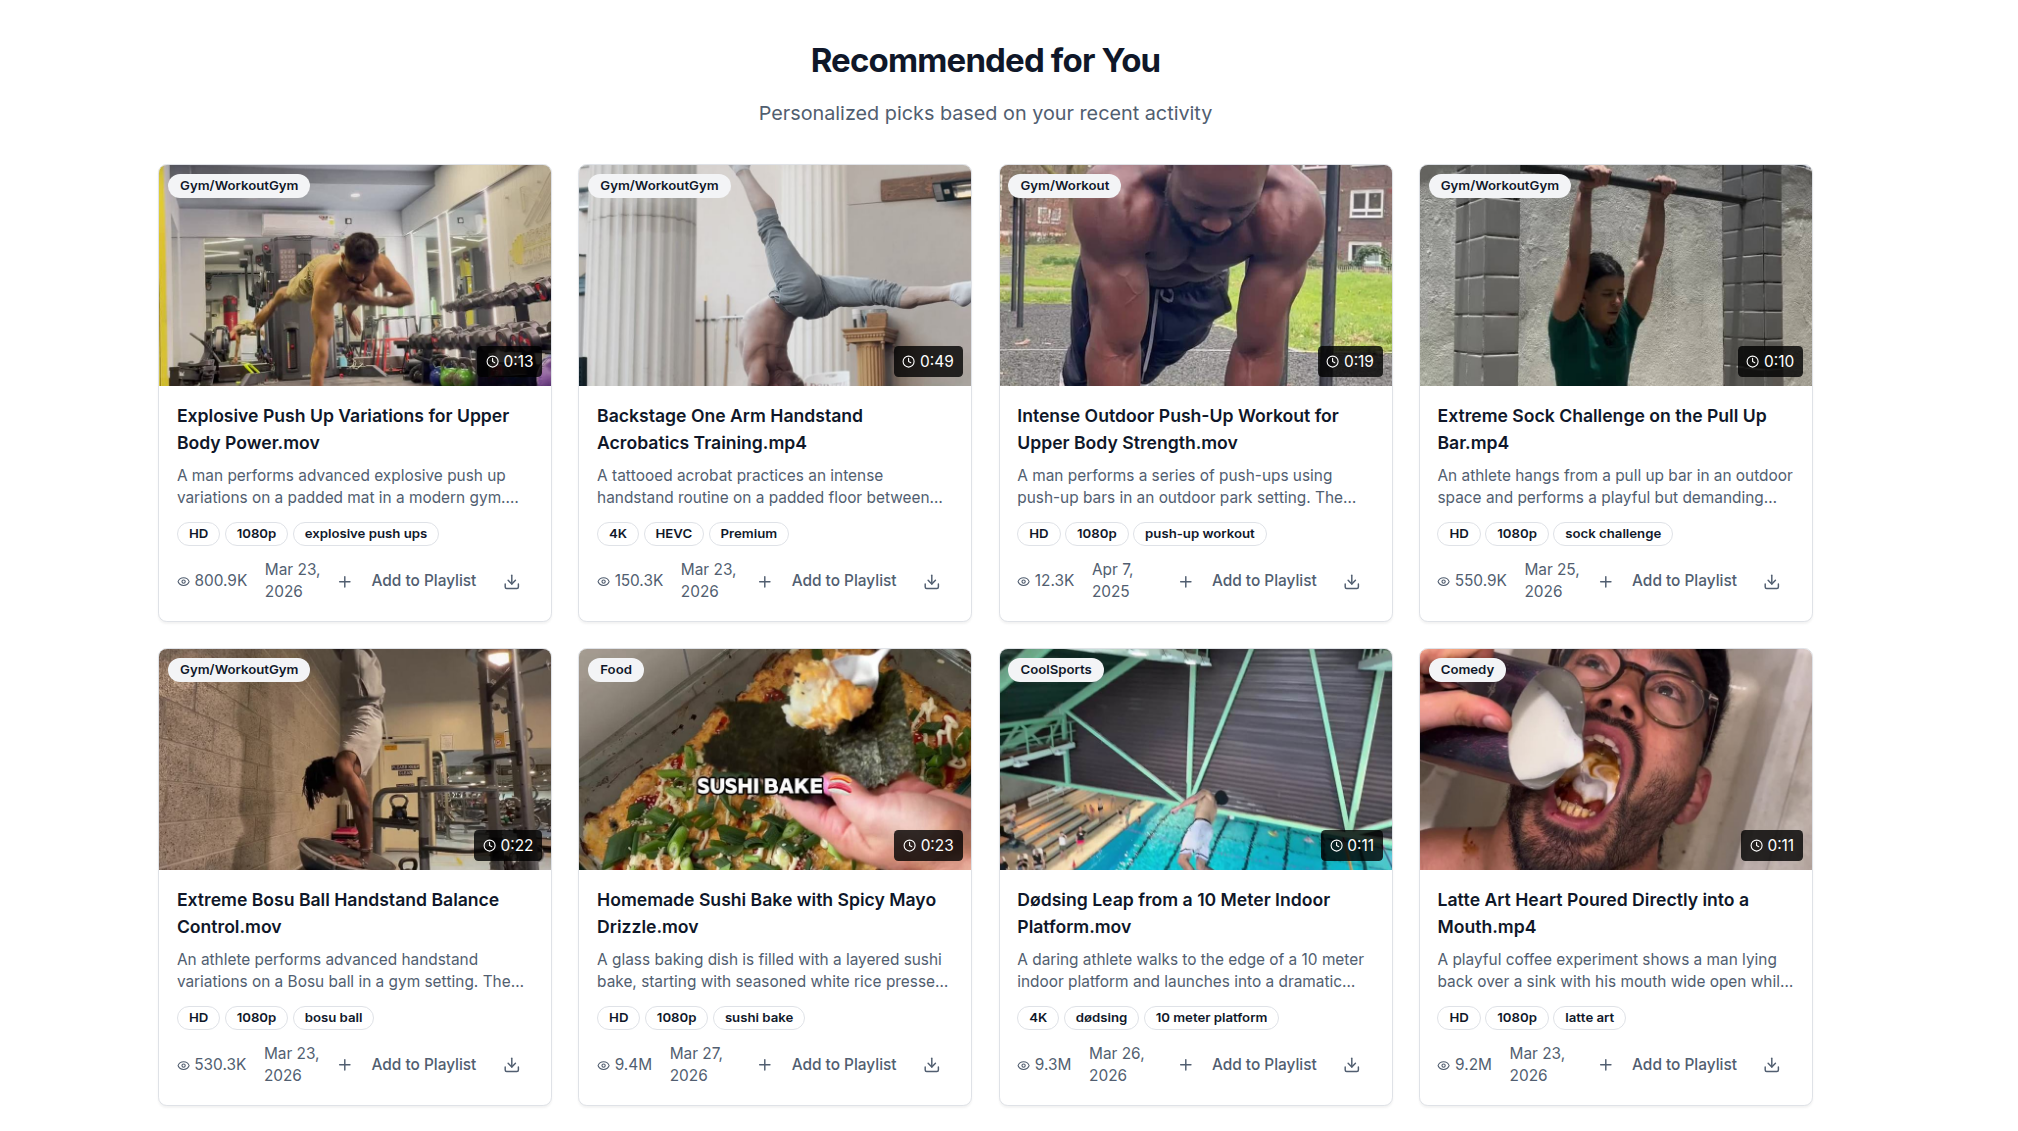
\includegraphics[width=\textwidth]{figures/videosearch/recommended for you page.png}
\caption{``Recommended for You'' section on the Video Search Portal home dashboard}
\label{fig:rec_ui}
\end{figure}

\section*{Conclusion}
\addcontentsline{toc}{section}{Conclusion}

Sprint 5 introduced a \textbf{personalized recommendation engine} driven by real-time
behavioural signals — search queries, click events, and playlist additions. A per-user interest
profile with exponential weight decay captures evolving preferences without requiring scheduled
recomputation jobs. The blended candidate pipeline, combining personalized and trending results
with freshness, diversity, and exploration controls, delivers a feed that improves with every
user interaction. Three new PostgreSQL tables and one Alembic migration extend the AR-API
schema, completing the personalization layer of the BVIRAL platform.

\chapter*{General Conclusion and Perspectives}
\addcontentsline{toc}{chapter}{General Conclusion and Perspectives}
\markboth{General Conclusion and Perspectives}{General Conclusion and Perspectives}

This internship marked a significant step in my academic and professional journey, consolidating
theoretical knowledge through practical work on a distributed microservices architecture with AI
integration. Developing the BVIRAL platform was an enriching experience that allowed me to
strengthen my skills with technologies such as FastAPI, Next.js, OpenSearch, Qdrant, and Docker.

Future evolution prospects for the project include:
\begin{itemize}
  \item \textbf{Multimodal video embedding pipeline}: Indexing thumbnails and transcripts with
    richer embeddings to enable scene-level semantic search.
  \item \textbf{LLM evaluation harness}: Building an offline evaluation suite to track RAG
    relevance, classifier accuracy, and hallucination rate across releases.
  \item \textbf{Deployment on Kubernetes}: Migrating from the current setup to Kubernetes for
    auto-scaling, stronger resilience, and high availability.
  \item \textbf{Advanced analytics dashboard}: Extending the admin dashboard with deeper usage,
    operational, and recommendation insights.
\end{itemize}

In summary, this internship concludes my university studies and fully prepares me to enter the
professional world. It has strengthened my software development skills and given me a solid
foundation to face future computer engineering challenges.


%% Back matter
\chapter*{Webography}
\markboth{Webography}{Webography}
\addcontentsline{toc}{chapter}{Webography}
\label{chap:webographie}
\pagestyle{empty}

The following web resources were consulted while writing this report, especially for presenting
the host organization, analyzing existing solutions, describing the technologies and tools used,
and documenting design and architecture choices.

\begin{enumerate}[leftmargin=0pt]

  \item \label{web:bviral} \textbf{BVIRAL Media Inc.} :
        \url{https://www.bviral.com/} (Accessed on January 15, 2026).\\
        Official website used to present the host organization and describe the viral video
        content licensing business model (Chapter~1, Section~1.1).

  \item \label{web:getty} \textbf{Getty Images} :
        \url{https://www.gettyimages.com/} (Accessed on January 20, 2026).\\
        Platform analyzed in the comparative study of existing video rights management and semantic
        search solutions (Chapter~1, Section~1.3).

  \item \label{web:storyful} \textbf{Storyful} :
        \url{https://storyful.com/} (Accessed on January 20, 2026).\\
        Social media monitoring platform analyzed as part of the state-of-the-art review, with a
        focus on manual licensing workflows (Chapter~1, Section~1.3).

  \item \label{web:jukin} \textbf{Jukin Media} :
        \url{https://www.jukinmedia.com/} (Accessed on January 21, 2026).\\
        Curated subscription-based video catalog solution analyzed in the comparative study
        (Chapter~1, Section~1.3).

  \item \label{web:shutterstock} \textbf{Shutterstock Video} :
        \url{https://www.shutterstock.com/video} (Accessed on January 21, 2026).\\
        International platform with semantic and filtered search analyzed for feature comparison
        (Chapter~1, Section~1.3).

  \item \label{web:scrumorg} \textbf{Scrum.org --- The Scrum Guide} :
        \url{https://www.scrum.org/resources/scrum-guide} (Accessed on January 25, 2026).\\
        Main reference for describing the Agile Scrum methodology and sprint process used in the
        project (Chapter~1, Section~1.4).

  \item \label{web:fastapi} \textbf{FastAPI} :
        \url{https://fastapi.tiangolo.com} (Accessed on February 1, 2026).\\
        Python framework used for AR-API and Agentic Helper.

  \item \label{web:flask} \textbf{Flask} :
        \url{https://flask.palletsprojects.com} (Accessed on February 1, 2026).\\
        Python framework used for the Videos Search API.

  \item \label{web:nextjs} \textbf{Next.js} :
        \url{https://nextjs.org/docs} (Accessed on February 2, 2026).\\
        React framework used for both portals and BFF routes (Chapters~2 and~7).

  \item \label{web:sqlalchemy} \textbf{SQLAlchemy} :
        \url{https://docs.sqlalchemy.org} (Accessed on February 3, 2026).\\
        Async Python ORM used for PostgreSQL access in FastAPI services.

  \item \label{web:alembic} \textbf{Alembic} :
        \url{https://alembic.sqlalchemy.org} (Accessed on February 3, 2026).\\
        Database migration tool used for AR-API schema evolution.

  \item \label{web:pydantic} \textbf{Pydantic} :
        \url{https://docs.pydantic.dev} (Accessed on February 4, 2026).\\
        Data validation library used for strict schemas and structured LLM outputs.

  \item \label{web:celery} \textbf{Celery} :
        \url{https://docs.celeryq.dev} (Accessed on February 5, 2026).\\
        Distributed task queue used for notifications and background processing.

  \item \label{web:radixui} \textbf{Radix UI} :
        \url{https://www.radix-ui.com} (Accessed on February 6, 2026).\\
        UI primitives used with Tailwind CSS in the Video Search Portal.

  \item \label{web:mui} \textbf{Material UI (MUI)} :
        \url{https://mui.com/material-ui/} (Accessed on February 6, 2026).\\
        UI component library used for dashboards and admin interfaces.

  \item \label{web:tailwind} \textbf{Tailwind CSS} :
        \url{https://tailwindcss.com/docs} (Accessed on February 6, 2026).\\
        Utility-first CSS framework used in the Video Search Portal.

  \item \label{web:langchain} \textbf{LangChain} :
        \url{https://python.langchain.com/docs/} (Accessed on February 10, 2026).\\
        LLM orchestration framework used for prompt chains and RAG.

  \item \label{web:langgraph} \textbf{LangGraph} :
        \url{https://langchain-ai.github.io/langgraph/} (Accessed on February 10, 2026).\\
        State-graph framework used for the video search ReAct agent.

  \item \label{web:langsmith} \textbf{LangSmith} :
        \url{https://smith.langchain.com/} (Accessed on February 11, 2026).\\
        Tracing and prompt management platform for Agentic Helper.

  \item \label{web:openai} \textbf{OpenAI API} :
        \url{https://platform.openai.com/docs/} (Accessed on February 12, 2026).\\
        API used for GPT models, embeddings, and Whisper transcription.

  \item \label{web:qdrant} \textbf{Qdrant} :
        \url{https://qdrant.tech/documentation/} (Accessed on February 14, 2026).\\
        Vector database used to store and retrieve semantic embeddings.

  \item \label{web:opensearch} \textbf{OpenSearch} :
        \url{https://opensearch.org/docs/} (Accessed on February 15, 2026).\\
        Search engine used for lexical, vector, and faceted video search.

  \item \label{web:clerk} \textbf{Clerk} :
        \url{https://clerk.com/docs} (Accessed on February 18, 2026).\\
        Authentication and user management service used across portals and AR-API.

  \item \label{web:stripe} \textbf{Stripe} :
        \url{https://stripe.com/docs} (Accessed on February 19, 2026).\\
        Payment platform used for checkout, subscriptions, and billing flows.

  \item \label{web:slack_api} \textbf{Slack Block Kit} :
        \url{https://api.slack.com/block-kit} (Accessed on February 20, 2026).\\
        Slack API used for structured notifications in backend workflows.

  \item \label{web:redis} \textbf{Redis} :
        \url{https://redis.io/docs/} (Accessed on February 22, 2026).\\
        In-memory data store used as Celery broker and state cache.

  \item \label{web:postgresql} \textbf{PostgreSQL} :
        \url{https://www.postgresql.org/docs/} (Accessed on February 22, 2026).\\
        Relational database used for core AR-API domain data.

  \item \label{web:docker} \textbf{Docker} :
        \url{https://docs.docker.com/} (Accessed on February 25, 2026).\\
        Containerization platform used to package services.

  \item \label{web:dockercompose} \textbf{Docker Compose} :
        \url{https://docs.docker.com/compose/} (Accessed on February 25, 2026).\\
        Local orchestration tool used to run the full stack.

  \item \label{web:python} \textbf{Python} :
        \url{https://docs.python.org/3/} (Accessed on March 2, 2026).\\
        Main backend language used in AR-API, Agentic Helper, and Videos Search API.

  \item \label{web:typescript} \textbf{TypeScript} :
        \url{https://www.typescriptlang.org/docs/} (Accessed on March 2, 2026).\\
        Main frontend language used in both Next.js portals.

  \item \label{web:postman} \textbf{Postman} :
        \url{https://www.postman.com/product/api-client/} (Accessed on March 4, 2026).\\
        API client used to test backend endpoints.

  \item \label{web:cursor} \textbf{Cursor IDE} :
        \url{https://www.cursor.com/} (Accessed on March 4, 2026).\\
        Primary AI-assisted code editor used during development.

  \item \label{web:vscode} \textbf{Visual Studio Code} :
        \url{https://code.visualstudio.com/docs} (Accessed on March 5, 2026).\\
        Secondary code editor used alongside Cursor IDE.

  \item \label{web:qdrant_cloud_console} \textbf{Qdrant Cloud Console} :
        \url{https://cloud.qdrant.io/} (Accessed on March 6, 2026).\\
        Web interface used to inspect and manage vector collections.

  \item \label{web:opensearch_dashboards} \textbf{OpenSearch Dashboards} :
        \url{https://opensearch.org/docs/latest/dashboards/} (Accessed on March 6, 2026).\\
        Visualization interface used to inspect OpenSearch indexes and queries.

  \item \label{web:pytest} \textbf{pytest} :
        \url{https://docs.pytest.org/} (Accessed on March 8, 2026).\\
        Python testing framework used for backend test suites.

\end{enumerate}


\end{document}
